% Options for packages loaded elsewhere
\PassOptionsToPackage{unicode}{hyperref}
\PassOptionsToPackage{hyphens}{url}
\PassOptionsToPackage{dvipsnames,svgnames,x11names}{xcolor}
%
\documentclass[
  letterpaper,
  DIV=11,
  numbers=noendperiod]{scrreprt}

\usepackage{amsmath,amssymb}
\usepackage{iftex}
\ifPDFTeX
  \usepackage[T1]{fontenc}
  \usepackage[utf8]{inputenc}
  \usepackage{textcomp} % provide euro and other symbols
\else % if luatex or xetex
  \usepackage{unicode-math}
  \defaultfontfeatures{Scale=MatchLowercase}
  \defaultfontfeatures[\rmfamily]{Ligatures=TeX,Scale=1}
\fi
\usepackage{lmodern}
\ifPDFTeX\else  
    % xetex/luatex font selection
\fi
% Use upquote if available, for straight quotes in verbatim environments
\IfFileExists{upquote.sty}{\usepackage{upquote}}{}
\IfFileExists{microtype.sty}{% use microtype if available
  \usepackage[]{microtype}
  \UseMicrotypeSet[protrusion]{basicmath} % disable protrusion for tt fonts
}{}
\makeatletter
\@ifundefined{KOMAClassName}{% if non-KOMA class
  \IfFileExists{parskip.sty}{%
    \usepackage{parskip}
  }{% else
    \setlength{\parindent}{0pt}
    \setlength{\parskip}{6pt plus 2pt minus 1pt}}
}{% if KOMA class
  \KOMAoptions{parskip=half}}
\makeatother
\usepackage{xcolor}
\setlength{\emergencystretch}{3em} % prevent overfull lines
\setcounter{secnumdepth}{2}
% Make \paragraph and \subparagraph free-standing
\ifx\paragraph\undefined\else
  \let\oldparagraph\paragraph
  \renewcommand{\paragraph}[1]{\oldparagraph{#1}\mbox{}}
\fi
\ifx\subparagraph\undefined\else
  \let\oldsubparagraph\subparagraph
  \renewcommand{\subparagraph}[1]{\oldsubparagraph{#1}\mbox{}}
\fi

\usepackage{color}
\usepackage{fancyvrb}
\newcommand{\VerbBar}{|}
\newcommand{\VERB}{\Verb[commandchars=\\\{\}]}
\DefineVerbatimEnvironment{Highlighting}{Verbatim}{commandchars=\\\{\}}
% Add ',fontsize=\small' for more characters per line
\usepackage{framed}
\definecolor{shadecolor}{RGB}{241,243,245}
\newenvironment{Shaded}{\begin{snugshade}}{\end{snugshade}}
\newcommand{\AlertTok}[1]{\textcolor[rgb]{0.68,0.00,0.00}{#1}}
\newcommand{\AnnotationTok}[1]{\textcolor[rgb]{0.37,0.37,0.37}{#1}}
\newcommand{\AttributeTok}[1]{\textcolor[rgb]{0.40,0.45,0.13}{#1}}
\newcommand{\BaseNTok}[1]{\textcolor[rgb]{0.68,0.00,0.00}{#1}}
\newcommand{\BuiltInTok}[1]{\textcolor[rgb]{0.00,0.23,0.31}{#1}}
\newcommand{\CharTok}[1]{\textcolor[rgb]{0.13,0.47,0.30}{#1}}
\newcommand{\CommentTok}[1]{\textcolor[rgb]{0.37,0.37,0.37}{#1}}
\newcommand{\CommentVarTok}[1]{\textcolor[rgb]{0.37,0.37,0.37}{\textit{#1}}}
\newcommand{\ConstantTok}[1]{\textcolor[rgb]{0.56,0.35,0.01}{#1}}
\newcommand{\ControlFlowTok}[1]{\textcolor[rgb]{0.00,0.23,0.31}{#1}}
\newcommand{\DataTypeTok}[1]{\textcolor[rgb]{0.68,0.00,0.00}{#1}}
\newcommand{\DecValTok}[1]{\textcolor[rgb]{0.68,0.00,0.00}{#1}}
\newcommand{\DocumentationTok}[1]{\textcolor[rgb]{0.37,0.37,0.37}{\textit{#1}}}
\newcommand{\ErrorTok}[1]{\textcolor[rgb]{0.68,0.00,0.00}{#1}}
\newcommand{\ExtensionTok}[1]{\textcolor[rgb]{0.00,0.23,0.31}{#1}}
\newcommand{\FloatTok}[1]{\textcolor[rgb]{0.68,0.00,0.00}{#1}}
\newcommand{\FunctionTok}[1]{\textcolor[rgb]{0.28,0.35,0.67}{#1}}
\newcommand{\ImportTok}[1]{\textcolor[rgb]{0.00,0.46,0.62}{#1}}
\newcommand{\InformationTok}[1]{\textcolor[rgb]{0.37,0.37,0.37}{#1}}
\newcommand{\KeywordTok}[1]{\textcolor[rgb]{0.00,0.23,0.31}{#1}}
\newcommand{\NormalTok}[1]{\textcolor[rgb]{0.00,0.23,0.31}{#1}}
\newcommand{\OperatorTok}[1]{\textcolor[rgb]{0.37,0.37,0.37}{#1}}
\newcommand{\OtherTok}[1]{\textcolor[rgb]{0.00,0.23,0.31}{#1}}
\newcommand{\PreprocessorTok}[1]{\textcolor[rgb]{0.68,0.00,0.00}{#1}}
\newcommand{\RegionMarkerTok}[1]{\textcolor[rgb]{0.00,0.23,0.31}{#1}}
\newcommand{\SpecialCharTok}[1]{\textcolor[rgb]{0.37,0.37,0.37}{#1}}
\newcommand{\SpecialStringTok}[1]{\textcolor[rgb]{0.13,0.47,0.30}{#1}}
\newcommand{\StringTok}[1]{\textcolor[rgb]{0.13,0.47,0.30}{#1}}
\newcommand{\VariableTok}[1]{\textcolor[rgb]{0.07,0.07,0.07}{#1}}
\newcommand{\VerbatimStringTok}[1]{\textcolor[rgb]{0.13,0.47,0.30}{#1}}
\newcommand{\WarningTok}[1]{\textcolor[rgb]{0.37,0.37,0.37}{\textit{#1}}}

\providecommand{\tightlist}{%
  \setlength{\itemsep}{0pt}\setlength{\parskip}{0pt}}\usepackage{longtable,booktabs,array}
\usepackage{calc} % for calculating minipage widths
% Correct order of tables after \paragraph or \subparagraph
\usepackage{etoolbox}
\makeatletter
\patchcmd\longtable{\par}{\if@noskipsec\mbox{}\fi\par}{}{}
\makeatother
% Allow footnotes in longtable head/foot
\IfFileExists{footnotehyper.sty}{\usepackage{footnotehyper}}{\usepackage{footnote}}
\makesavenoteenv{longtable}
\usepackage{graphicx}
\makeatletter
\def\maxwidth{\ifdim\Gin@nat@width>\linewidth\linewidth\else\Gin@nat@width\fi}
\def\maxheight{\ifdim\Gin@nat@height>\textheight\textheight\else\Gin@nat@height\fi}
\makeatother
% Scale images if necessary, so that they will not overflow the page
% margins by default, and it is still possible to overwrite the defaults
% using explicit options in \includegraphics[width, height, ...]{}
\setkeys{Gin}{width=\maxwidth,height=\maxheight,keepaspectratio}
% Set default figure placement to htbp
\makeatletter
\def\fps@figure{htbp}
\makeatother
\newlength{\cslhangindent}
\setlength{\cslhangindent}{1.5em}
\newlength{\csllabelwidth}
\setlength{\csllabelwidth}{3em}
\newlength{\cslentryspacingunit} % times entry-spacing
\setlength{\cslentryspacingunit}{\parskip}
\newenvironment{CSLReferences}[2] % #1 hanging-ident, #2 entry spacing
 {% don't indent paragraphs
  \setlength{\parindent}{0pt}
  % turn on hanging indent if param 1 is 1
  \ifodd #1
  \let\oldpar\par
  \def\par{\hangindent=\cslhangindent\oldpar}
  \fi
  % set entry spacing
  \setlength{\parskip}{#2\cslentryspacingunit}
 }%
 {}
\usepackage{calc}
\newcommand{\CSLBlock}[1]{#1\hfill\break}
\newcommand{\CSLLeftMargin}[1]{\parbox[t]{\csllabelwidth}{#1}}
\newcommand{\CSLRightInline}[1]{\parbox[t]{\linewidth - \csllabelwidth}{#1}\break}
\newcommand{\CSLIndent}[1]{\hspace{\cslhangindent}#1}

\DeclareMathOperator{\logit}{logit}
\DeclareMathOperator{\Var}{Var}
\DeclareMathOperator{\SE}{SE}
\newcommand{\given}{\,|\,}
\newcommand{\indep}{\perp\!\!\!\!\perp}
\newcommand\diff{\mathop{}\!\mathrm{d}}
\newcommand\Diff[1]{\mathop{}\!\mathrm{d^#1}}

% \usepackage[Sonny]{fncychap} % Only works with class: book

\usepackage{booktabs}
\usepackage{longtable}
\usepackage{array}
\usepackage{multirow}
\usepackage{wrapfig}
\usepackage{float}
\usepackage{colortbl}
\usepackage{pdflscape}
\usepackage{tabu}
\usepackage{threeparttable}
\usepackage{threeparttablex}
\usepackage[normalem]{ulem}
\usepackage{makecell}
\usepackage{xcolor}
\KOMAoption{captions}{tableheading}
\makeatletter
\makeatother
\makeatletter
\@ifpackageloaded{bookmark}{}{\usepackage{bookmark}}
\makeatother
\makeatletter
\@ifpackageloaded{caption}{}{\usepackage{caption}}
\AtBeginDocument{%
\ifdefined\contentsname
  \renewcommand*\contentsname{Table of contents}
\else
  \newcommand\contentsname{Table of contents}
\fi
\ifdefined\listfigurename
  \renewcommand*\listfigurename{List of Figures}
\else
  \newcommand\listfigurename{List of Figures}
\fi
\ifdefined\listtablename
  \renewcommand*\listtablename{List of Tables}
\else
  \newcommand\listtablename{List of Tables}
\fi
\ifdefined\figurename
  \renewcommand*\figurename{Figure}
\else
  \newcommand\figurename{Figure}
\fi
\ifdefined\tablename
  \renewcommand*\tablename{Table}
\else
  \newcommand\tablename{Table}
\fi
}
\@ifpackageloaded{float}{}{\usepackage{float}}
\floatstyle{ruled}
\@ifundefined{c@chapter}{\newfloat{codelisting}{h}{lop}}{\newfloat{codelisting}{h}{lop}[chapter]}
\floatname{codelisting}{Listing}
\newcommand*\listoflistings{\listof{codelisting}{List of Listings}}
\makeatother
\makeatletter
\@ifpackageloaded{caption}{}{\usepackage{caption}}
\@ifpackageloaded{subcaption}{}{\usepackage{subcaption}}
\makeatother
\makeatletter
\@ifpackageloaded{tcolorbox}{}{\usepackage[skins,breakable]{tcolorbox}}
\makeatother
\makeatletter
\@ifundefined{shadecolor}{\definecolor{shadecolor}{rgb}{.97, .97, .97}}
\makeatother
\makeatletter
\makeatother
\makeatletter
\makeatother
\ifLuaTeX
  \usepackage{selnolig}  % disable illegal ligatures
\fi
\IfFileExists{bookmark.sty}{\usepackage{bookmark}}{\usepackage{hyperref}}
\IfFileExists{xurl.sty}{\usepackage{xurl}}{} % add URL line breaks if available
\urlstyle{same} % disable monospaced font for URLs
\hypersetup{
  pdftitle={Advances in competing risks and missing data},
  pdfauthor={Edouard F Bonneville},
  colorlinks=true,
  linkcolor={blue},
  filecolor={Maroon},
  citecolor={Blue},
  urlcolor={Blue},
  pdfcreator={LaTeX via pandoc}}

\title{Advances in competing risks and missing data}
\usepackage{etoolbox}
\makeatletter
\providecommand{\subtitle}[1]{% add subtitle to \maketitle
  \apptocmd{\@title}{\par {\large #1 \par}}{}{}
}
\makeatother
\subtitle{With applications to allogeneic stem cell transplantation}
\author{Edouard F Bonneville}
\date{}

\begin{document}
\maketitle
\ifdefined\Shaded\renewenvironment{Shaded}{\begin{tcolorbox}[enhanced, sharp corners, frame hidden, interior hidden, borderline west={3pt}{0pt}{shadecolor}, boxrule=0pt, breakable]}{\end{tcolorbox}}\fi

\renewcommand*\contentsname{Table of contents}
{
\hypersetup{linkcolor=}
\setcounter{tocdepth}{1}
\tableofcontents
}
\listoffigures
\listoftables
\bookmarksetup{startatroot}

\hypertarget{preface}{%
\chapter*{Preface}\label{preface}}
\addcontentsline{toc}{chapter}{Preface}

\markboth{Preface}{Preface}

This is a Quarto document.

To learn more about Quarto books visit
\url{https://quarto.org/docs/books}.

\begin{Shaded}
\begin{Highlighting}[]
\DecValTok{1} \SpecialCharTok{+} \DecValTok{1}
\end{Highlighting}
\end{Shaded}

\begin{verbatim}
[1] 2
\end{verbatim}

\bookmarksetup{startatroot}

\hypertarget{general-introduction}{%
\chapter{General Introduction}\label{general-introduction}}

\hypertarget{outline-of-this-thesis}{%
\section{Outline of this thesis}\label{outline-of-this-thesis}}

In chapter bla we will bla. That's about it really. And some more.

\bookmarksetup{startatroot}

\hypertarget{handling-missing-covariate-data-in-clinical-studies-in-haematology}{%
\chapter{Handling missing covariate data in clinical studies in
haematology}\label{handling-missing-covariate-data-in-clinical-studies-in-haematology}}

Missing data are frequently encountered across studies in clinical
haematology. Failure to handle these missing values in an appropriate
manner can complicate the interpretation of a study's findings, as
estimates presented may be biased and/or imprecise. In the present work,
we first provide an overview of current methods for handling missing
covariate data, along with their advantages and disadvantages.
Furthermore, a systematic review is presented, exploring both
contemporary reporting of missing values in major haematological
journals, and the methods used for handling them. A principle finding
was that the method of handling missing data was explicitly specified in
a minority of articles (in 76 out of 195 articles reporting missing
values, 39\%). Among these, complete case analysis and the missing
indicator method were the most common approaches to dealing with missing
values, with more complex methods such as multiple imputation being
extremely rare (in 7 out of 195 articles). An example analysis (with
associated code) is also provided using haematopoietic stem cell
transplant data, illustrating the different approaches to handling
missing values. We conclude with various recommendations regarding the
reporting and handling of missing values for future studies in clinical
haematology.

\hfill\break

\hypertarget{introduction}{%
\section{Introduction}\label{introduction}}

Missing data are widely encountered in clinical research across both
covariate and outcome information. For example, a patient known to have
relapsed from a particular malignant disease may be lacking information
on the precise timing of the relapse (missing outcome), but may also
have incomplete data on important prognostic factors that may be
time-consuming or expensive to collect, or were not considered relevant
at the moment of diagnosis or start of treatment (missing covariate).

While missing values generally represent a nuisance to the researcher,
failure to adequately account for them may lead to results that are
potentially biased and/or imprecise
(\protect\hyperlink{ref-sterneMultipleImputationMissing2009}{Sterne
\emph{et al.}, 2009}). Insufficient reporting of missing values may also
complicate the interpretation of a study's results. Both the reporting
of missing values and the methods used for handling them have been the
subject of multiple reviews across a multitude of study types and
outcome models (\protect\hyperlink{ref-bellHandlingMissingData2014}{Bell
\emph{et al.}, 2014};
\protect\hyperlink{ref-burtonMissingCovariateData2004}{Burton and
Altman, 2004}; \protect\hyperlink{ref-carrollHowAreMissing2020}{Carroll
\emph{et al.}, 2020};
\protect\hyperlink{ref-sullivanTreatmentMissingData2017}{Sullivan
\emph{et al.}, 2017}).

On the subject of clinical studies in haematology, there has to the best
of our knowledge been no explicit investigation into contemporary
reporting and handling of missing data. Similarly, field-specific
guidelines seem to be restricted to a section from Delgado et al., which
are limited in scope and arguably outdated
(\protect\hyperlink{ref-delgadoSurvivalAnalysisHematologic2014}{Delgado
\emph{et al.}, 2014}). The present work seeks to fill this knowledge
gap, focusing mainly on missing covariate data. We will first introduce
the assumptions underlying missing data, as well as the common methods
used to handle them and their associated pitfalls. We follow this up
with a systematic review of missing data related practices across major
haematological journals, and an applied data example. We then conclude
with recommendations for further practice.

\hypertarget{assumptions-underlying-methods-for-handling-missing-data}{%
\section{Assumptions underlying methods for handling missing
data}\label{assumptions-underlying-methods-for-handling-missing-data}}

Any discussion concerning missing values in the context of a particular
study should always begin with one simple question: why are the values
missing? This enquiry into the possible causes of the missing values is
in fact an assessment of the missing data mechanism. Little and Rubin
formalized the concept, assuming that every value a priori had some
probability of becoming missing, which could depend on either observed
or unobserved information
(\protect\hyperlink{ref-littleStatisticalAnalysisMissing2019}{Little and
Rubin, 2019}).

Suppose that in the context of a retrospective study, performance status
(measured for example by means of the Karnofsky Performance Score, KPS)
is missing for a portion of the patient cohort. These values are missing
completely at random (MCAR) when all patients are equally likely to have
a missing value. That is, no one subgroup defined by the data
(e.g.~older patients) has any comparatively higher likelihood of having
a missing KPS value. The missingness is independent from both observed
and unobserved information.

In the case where observed information fully explains whether the data
are missing or not, we refer to the mechanism as missing at random
(MAR). For example, younger patients may have their KPS score recorded
less routinely than older patients. In other words, whether or not the
KPS score is observed can be explained using the observed age
information. If the missing data are related to unobserved information,
we refer to them as missing not at random (MNAR). An example of this
would be if patients with a higher KPS score would also have a higher
likelihood of having a corresponding missing value, e.g., because fitter
-- but not necessarily younger - patients are monitored less
intensively. The missingness in this example is therefore related to the
unobserved KPS values or patient fitness not measured by any other
variable.

Given that MNAR data by definition depends on unobserved information, it
is impossible to distinguish from MAR data based on data alone. Since
the most common missing data handling methods will rely on data being
MAR, it is critical to discuss how plausible the assumption is in a
given context. Such a discussion should take place not only between
statisticians and researchers, but also together with data managers, and
other persons who possess intimate knowledge of the data collection
process.

\hypertarget{common-approaches-and-associated-pitfalls}{%
\section{Common approaches and associated
pitfalls}\label{common-approaches-and-associated-pitfalls}}

In what follows, we outline common approaches for handling missing
values in the context of a regression model - referred to as the
analysis or substantive model. We assume that the outcome of the model
is observed for all individuals, and that one or more of the predictors
used have missing values.

\hypertarget{complete-case-analysis}{%
\subsection{Complete case analysis}\label{complete-case-analysis}}

The simplest solution to deal with missing covariate data is to perform
a complete case analysis (CCA). This excludes patients from an analysis
as soon as they have an unknown value on at least one of the predictor
variables. Therefore, in a multivariable analysis model with missingness
spanning multiple predictors, the potential loss in statistical
precision can be substantial -- as reflected by wide confidence
intervals. While a CCA is valid under the assumption of MCAR, it is also
unbiased in various MAR and even MNAR situations
(\protect\hyperlink{ref-hughesAccountingMissingData2019}{Hughes \emph{et
al.}, 2019}). In turn, when missingness depends on the outcome, or
observed variables explaining the missingness are not accounted for
(e.g.~by adjusting for them in a multivariable model), CCA will
generally be biased. That is, the estimate(s) obtained using CCA will
differ with respect to those that would have been obtained had the data
been complete. Note also that CCA is the (often implicit) default
strategy for handling missing values in most software packages.

\hypertarget{missing-indicator-method}{%
\subsection{Missing indicator method}\label{missing-indicator-method}}

A straightforward way to exploit all available data is to use the
missing indicator method (MIM). For categorical variables, this simply
involves creating an additional level for the missing values. For
continuous variables, the missing values are first replaced by a
constant (commonly zero, or the observed average), and thereafter a
binary variable indicating whether the value was missing in the first
place or not is added to the model. Two major advantages of this method
are that the patients with missing information are monitored in
univariable analyses (e.g.~checking whether those with missing data have
much higher or lower overall survival compared to those with observed
information), and that it retains all information for multivariable
modelling. The MIM has historically been criticized, as it has been
shown to potentially be biased, even in cases with data that are MCAR
(\protect\hyperlink{ref-dondersReviewGentleIntroduction2006}{Donders
\emph{et al.}, 2006}). Nevertheless, it may prove to be a pragmatic
solution under particular assumptions and mild confounding
(\protect\hyperlink{ref-blakeEstimatingTreatmentEffects2020}{Blake
\emph{et al.}, 2020}).

\hypertarget{single-imputation}{%
\subsection{Single imputation}\label{single-imputation}}

One may also choose to replace all missing values in a variable (for
example by the average among observed values) and proceed to analyze the
data as if they were complete. This type of single imputation is
generally discouraged as it does not take into account any of the
uncertainty regarding the missing values
(\protect\hyperlink{ref-sterneMultipleImputationMissing2009}{Sterne
\emph{et al.}, 2009}). Data are analyzed as if they were complete
(i.e.~failing to capture that each missing value could have taken a
range of different values, other than for example the observed average),
leading to confidence intervals that are too narrow. A less well known
instance of single imputation occurs in categorical variables, where the
analyst may choose to combine those individuals with missing values
together with another factor level, usually the most frequent one. This
may in fact also occur at a pre-processing stage, as may be the case for
the calculation of the disease risk index (DRI), used in registry
studies about patients undergoing allogeneic stem cell transplantation
(alloSCT)
(\protect\hyperlink{ref-armandValidationRefinementDisease2014}{Armand
\emph{et al.}, 2014}). In different implementations of the DRI, patients
with myelodysplastic syndromes or acute myeloid leukemia lacking
cytogenetic risk classification (a component of the DRI) are assumed to
belong to (i.e.~singly imputed as) the most commonly observed category,
intermediate cytogenetic risk
(\protect\hyperlink{ref-armandDiseaseRiskIndex2012}{Armand \emph{et
al.}, 2012};
\protect\hyperlink{ref-saccardiBenchmarkingSurvivalOutcomes2023}{Saccardi
\emph{et al.}, 2023};
\protect\hyperlink{ref-snowdenBenchmarkingSurvivalOutcomes2020}{Snowden
\emph{et al.}, 2020}). In the original implementation of the DRI, this
was justified on the basis of outcomes being similar between those
unavailable and intermediate cytogenetics. Note also that the MIM is not
a form of single imputation: it assumes (in the case of a categorical
variable), that missing values belong to a separate category, rather
than to any one of the existing categories.

\hypertarget{multiple-imputation}{%
\subsection{Multiple imputation}\label{multiple-imputation}}

A more complex strategy to handle missing values is multiple imputation
(MI). MI leverages the observed data to repeatedly replace the missing
values by plausible (model-based) values. Doing so results in multiple
`complete' datasets that can separately be analyzed, and whose results
can be combined in a way that properly accounts for the uncertainty
induced by the missing values (using so-called Rubin's rules). MI is one
of multiple missing data methods that operate under the MAR assumption,
and are capable of producing more precise estimates compared to CCA
(\protect\hyperlink{ref-whiteBiasEfficiencyMultiple2010}{White and
Carlin, 2010}).

There are different variants of MI, of which the best known is
multivariate imputation by chained equations (MICE)
(\protect\hyperlink{ref-vanbuurens.FlexibleMultivariateImputation1999}{van
Buuren, S. \emph{et al.}, 1999}), implemented for example in the `mice'
R package
(\protect\hyperlink{ref-buurenMiceMultivariateImputation2011}{Buuren and
Groothuis-Oudshoorn, 2011}). For each variable with missing data, an
imputation model needs to be specified and fitted using the observed
part of the variable, and can thereafter be used to generate imputed
values. This approach allows to flexibly specify different models for
different variable types, such as a logistic regression if the variable
to be imputed is binary. Once these models are specified, there are two
main settings to fix: the number of imputed datasets, and the number of
iterations (also known as cycles). To generate a single imputed dataset,
MICE will start with an initial guess for each missing value by choosing
randomly from the observed values. Naturally, these initial guesses may
be far from values we could have expected given a patient's other
variables: for example, initial guesses for KPS scores among younger
patients could be low due to the random choice, when we might have
plausibly expected them to be high. In order to move in the direction of
more plausible values given the observed data, we `chain' the imputation
models together: the most recently imputed values are used as predictors
in the imputation model for the next variable to be imputed. One pass
across all variables with missing data represents a single cycle or
iteration. It is necessary to continue these cycles (i.e.~imputed values
at the end of the first cycle are used as starting values for the second
cycle, and so forth) until `convergence' is reached, i.e.~the sequence
of imputed values generated has stabilized. The imputed values at the
end of the final cycle form a single imputed dataset. Independent
(i.e.~with different starting values) runs of these cycles give rise to
multiple imputed datasets.

In studies where missing data are abundant, it is crucial to pick a
sufficiently large number of imputed datasets. When the proportion of
missing data is high, the imputation models are fitted on a smaller
portion of data, which will lead to a larger variability in the imputed
values. Intuitively, we need to make sure that conclusions made on the
basis of for example 10 imputed datasets, do not substantially differ
from those that would have been made under another set of 10 imputed
datasets (i.e.~had we repeated the entire multiple imputation
procedure). A rule of thumb is to use as many imputed datasets as the
percentage of incomplete observations (e.g.~40 imputed datasets if a CCA
discards 40\% of observations), although recent research suggests that
the number of imputed datasets should be even larger
(\protect\hyperlink{ref-mertensConstructionAssessmentPrediction2020}{Mertens
\emph{et al.}, 2020};
\protect\hyperlink{ref-vonhippelHowManyImputations2020}{von Hippel,
2020}). Generally, at least 10-20 iterations are recommended, and
convergence should be assessed using visual diagnostic tools, such as
those described in section 6.4.2 of the text by van Buuren
(\protect\hyperlink{ref-buurenFlexibleImputationMissing2018}{van Buuren,
2018}).

Another key consideration in MI is the issue of compatibility between
analysis and imputation models, that is, that the imputation models
should make assumptions that are consistent with those made by the
proposed analysis model. Practically speaking, this means that all
variables in the analysis model, including the outcome, should also be
included as predictors in the imputation model. It also means that
special terms, such as interactions, should be adequately handled. A
version of MICE which naturally ensures compatibility between the
analysis and imputation models in such situations is
substantive-model-compatible fully conditional specification
(SMC-FCS)(\protect\hyperlink{ref-bartlettMultipleImputationCovariates2015}{Bartlett
\emph{et al.}, 2015}), implemented in the `smcfcs' R package
(\protect\hyperlink{ref-bartlettSmcfcsMultipleImputation2022}{Bartlett
\emph{et al.}, 2022}).

A closely related approach to SMC-FCS is fully Bayesian imputation,
implemented in the `JointAI' R package
(\protect\hyperlink{ref-erlerJointAIJointAnalysis2021}{Erler \emph{et
al.}, 2021}). This performs analysis and imputation simultaneously,
again ensuring compatibility between the imputation and analysis models.
An overview of these and related methods are found in the work of
Carpenter and Smuk
(\protect\hyperlink{ref-carpenterMissingDataStatistical2021}{Carpenter
and Smuk, 2021}).

Research concerning the theory and performance of different MI
approaches extends to the field of survival analysis, with particular
focus on the widely-used Cox proportional hazards model. When the
analysis model of interest is a Cox model, White and Royston
(\protect\hyperlink{ref-whiteImputingMissingCovariate2009}{White and
Royston, 2009}) suggested that the imputation model for a partially
observed variable should include as predictors the remaining covariates
from the analysis model, the event indicator (indicating whether an
patient experienced an event or was censored) and the Nelson-Aalen
estimate of the cumulative hazard. This approach is expected to work
well in settings with a low cumulative incidence, and when the true
effects of the covariates are small. When this does not hold, results
are expected to be biased: the imputation and analysis model are only
approximately compatible. That is, this imputation model produces
imputed values which are not completely consistent with data where the
key assumption made by a Cox model (multiplicative covariate effects on
the hazard) is assumed to hold.

The SMC-FCS approach, which addresses this compatibility issue directly,
has shown superior performance (when the analysis model is well
specified) compared to the standard MICE approach described in the
previous paragraph across multiple simulation studies, including
settings with time-varying effects of covariates
(\protect\hyperlink{ref-keoghMultipleImputationCox2018}{Keogh and
Morris, 2018}), excess hazard models
(\protect\hyperlink{ref-antunesDealingMissingInformation2021}{Antunes
\emph{et al.}, 2021}), and competing risks
(\protect\hyperlink{ref-bartlettMissingCovariatesCompeting2016}{Bartlett
and Taylor, 2016};
\protect\hyperlink{ref-bonnevilleMultipleImputationCausespecific2022}{Bonneville
\emph{et al.}, 2022}). While to our knowledge there has been no
systematic evaluation of the fully Bayesian approach in the context of
the Cox model, the expectation is that it should perform at least as
well as the SMC-FCS approach. This is because it not only ensures that
the imputations are consistent with the analysis model, but also that
the different imputation models (when there are multiple variables to be
imputed) are consistent with each other. The latter point may be of
concern when there are complex non-linear relationships between
covariates.

\hypertarget{systematic-review}{%
\section{Systematic review}\label{systematic-review}}

\hypertarget{search-strategy-and-data-extraction}{%
\subsection{Search strategy and data
extraction}\label{search-strategy-and-data-extraction}}

We performed a systematic review to obtain a broad picture of current
practices in missing data reporting and handling across research
articles published in major haematological journals. We used the Ovid
platform to search the MEDLINE and Embase databases for articles written
in English in 2021. We excluded articles that did not contain new data
analyses (such as review articles), as well as letters to the editor,
since their brevity would preclude full reporting on the issues we are
interested in. Meta-analyses, methodological publications and articles
that were co-authored by authors of the present work were also excluded.
A total of 16 journals were selected, based on two primary criteria: a
5-year Journal Impact Factor (2021) larger than 3 (data obtained via
Journal Citation Reports Science Edition, Clarivate Analytics 2018), and
a journal scope focused on clinical research in haematological
malignancies. The 5-year Journal Impact Factor criteria was used in
order to target articles with (on average) better quality of methodology
and reporting, and a larger readership.

The search terms in Ovid format are reported in Table 1. After narrowing
down by journals and year of publication, the remaining criteria focused
on the malignant disease group, and the type of analysis model used. A
wide selection of malignant diseases was included: acute and chronic
myeloid leukemia, acute and chronic lymphocytic leukemia,
myelodysplastic syndromes (MDS), and non-Hodgkin lymphomas (NHL) . We
searched for articles that used a multivariable Cox proportional hazards
model as part of their statistical analysis. Models were further
classified into standard Cox, Fine-Gray (competing risks), frailty,
multi-state and relative survival. The standard Cox category included
standard outcomes such as overall or progression-free survival, but also
cause-specific Cox models for outcomes such as relapse incidence and
non-relapse mortality (since these are applied by treating competing
risks as censored). Search terms for both analysis model and malignant
disease group were based on detection of relevant strings in either
title, abstract or keywords.

\hypertarget{tbl-ovid-search}{}
\begin{table}
\caption{\label{tbl-ovid-search}Search terms used in Ovid format, as entered into MEDLINE and Embase. }\tabularnewline

\centering
\begin{tabular}[t]{l>{\raggedright\arraybackslash}p{35em}}
\toprule
 & \\
\midrule
1. & (0006-4971 or 2352-3026 or 1756-8722 or 2044-5385 or 0887-6924 or 0390-6078 or 0361-8609 or 2473-9529 or 0007-1048 or 2666-6367 or 0268-3369 or 2040-6207 or 0278-0232 or 0939-5555 or 1545-5009 or 1042-8194).is.\\
2. & (cox or HR or aHR or (hazard adj1 ratio) or hazard or (proportional adj1 hazards) or multivaria*).ti,ab,kf.\\
3. & ((acute adj1 myeloid adj1 leukemia) or (myelodysplastic adj1 syndrome*) or (chronic adj1 lymphocytic adj1 leukemia) or non-Hodgkin* or (chronic adj1 myeloid adj1 leukemia) or (acute adj1 lymphocytic adj1 leukemia) or (multiple adj1 myeloma) or leukem* or leukaem*).ti,ab,kf.\\
4. & 1 and 2 and 3\\
5. & limit 4 to ('conference review' or 'review')\\
6. & limit 4 to (article or article in press or journal article)\\
7. & 6 not 5\\
8. & limit 7 to english language\\
9. & limit 8 to yr='2021 - 2021'\\
10. & remove duplicates from 9\\
\bottomrule
\end{tabular}
\end{table}

For each included article, the information extraction spanned three main
areas: 1) exclusion of patients at `population selection' phase based on
missing data, 2) presence and explicit reporting of missing data in
baseline covariates used in one or more of the reported analysis models,
and 3) explicit reporting of methods used to handle the missing data.
The first part of the extraction is based on the findings in
(\protect\hyperlink{ref-carrollHowAreMissing2020}{Carroll \emph{et al.},
2020}), namely that the population is occasionally filtered on the basis
of information/variable availability, leaving little or no missing data
at the analysis phase. Two possible examples of this are, a)
retrospective analysis of data from multiple trials, and a particular
trial being excluded because information on a covariate of interest was
not collected; b) in a retrospective study, including only those with
sequencing data at a point in time (thereby implicitly excluding those
with unavailable sequencing data).

We checked whether there was any missing data in any of the covariates
making up the multivariable model, whether it be reported in the
descriptive `Table 1' (hereafter referred to as the `descriptives
table'), in a figure or in the main text. If there were multiple
multivariable Cox models reported in the article, we recorded whether in
at least one of them there was a covariate with missing data. Note that
sometimes the missing values are only implicitly reported, as is for
example the case when the numbers per level of categorical variables are
reported, and these fail to add up to the total.

In terms of missing data handling, we paid particular attention to the
use of CCA. Specifically, when missing values are reported, authors can
be explicit about use of complete cases in two main ways: specifying the
number of subjects used when reporting the multivariable model, or
including a sentence in-text explicitly mentioning the use of CCA (the
sentence `missing values were not imputed' is also appropriate).
Otherwise, the use of CCA was considered implicit - which can be
problematic since the reader is unaware of the extent of the power loss.
Likewise, we also recorded whether other methods were used, such as:
MIM, single imputation, MI or other. We also recorded the software used
for the analysis. The full extraction sheet is available in the online
supplement.

An initial investigation was carried out by EB, LdW and HP using 10
randomly selected papers. This was done in order to assess the
consistency of data extraction, sharpen the data extraction checklist
and agree on how to extract information when answers were ambiguous.
Data extraction was then carried out by EB.

\hypertarget{results}{%
\subsection{Results}\label{results}}

A total of 398 research articles were identified after eliminating
duplicate records obtained via MEDLINE (n = 86) and Embase (n = 391).
From those, 99 were excluded due to either co-authors of the present
manuscript being involved as co-author on the publication (n = 8),
meta-analyses (n = 6), no Cox models reported (n = 48) and absence of
multivariable Cox model (n = 36). One article was excluded as the
supplementary material (which described the predictors used in the
multivariable model) was not available on the publisher's website. A
total of 299 articles were therefore included in the review. The
journals where these articles most frequently featured in were Bone
Marrow Transplantation (n = 46), Transplantation and Cellular Therapy (n
= 40), Blood Advances (n = 35), Annals of Hematology (n = 33), and
Leukemia and Lymphoma (n = 28).

At population selection, 80 articles (27\%) explicitly reported having
excluded observations on the basis of missing information. At this stage
of the extraction, the focus was not yet solely on covariates that would
make part of the multivariable model(s) in a particular article. These
80 articles could thus for example comprise exclusions based on missing
outcome data. Given the retrospective nature of many studies, many of
these exclusions were based on lack of cytogenetic information or no
minimal residual disease (MRD) assessments, as was the case (exclusion
of patients without cytogenetic information) for example in Hansen D.K.
\emph{et al.}
(\protect\hyperlink{ref-hansend.k.ELN2017Genetic2021}{2021}). It is
important to note that while this approach can seem natural, it could
come at the cost of ending up with a slightly different population than
the one originally targeted. A possible sanity test would be to compare
the univariable outcomes (e.g.~Kaplan-Meier based overall survival)
between those excluded and those remaining.

The vast majority of articles (287 out of 299, 96\%) included at least
one standard Cox model. The Fine-Gray model for competing risks was used
in 69 articles (23\%), and frailty models were employed in 14 articles.
Multi-state models (n = 2) and relative survival approaches (n = 3) were
rarely employed. Furthermore, the software used for the analyses was R
(n = 144), SPSS (n = 94), SAS (n = 55), Stata (n = 35), unknown/ not
specified (n = 40), and other (n = 28). These numbers do not add up to
the total as 86 articles used two or more of these software packages in
combination.

A total of 195 articles (65\%) reported missing data in at least one of
the covariates that formed part of one or more of the presented
multivariable models. In most cases, these were explicitly reported in
the descriptives table (n = 124), in both the descriptives table and in
text (n = 24) and in the main text only (n = 19). In some instances,
these were reported as part of a figure/flowchart (n = 3) The missing
values (for at least one of the variables) were implicit in 20 articles,
deducted based on subcategories in the descriptives table not adding up
to totals.

In 39\% (n = 76) of the 195 articles reporting missing values, the
method (or at least one of the methods, if multiple were used) for
handling missing data was explicitly specified. The most common methods
for dealing with missing values among these were CCA (n = 34), MIM (n =
29), MI (n = 6) and single imputation (n = 5). One article used both MIM
and CCA together, while another used both MI and CCA. Han S.Y. \emph{et
al.}
(\protect\hyperlink{ref-hans.y.SecondaryCytogeneticAbnormalities2021}{2021})
provide a clear example of explicit method reporting in-text: they
mention the use of MIM for a particular mutation status indicator, and
the use of CCA on the remaining variables with missing values.
Furthermore, in that same study, treatment data was not available for
all patients: they proceeded to compare survival outcomes of patients
with and without available treatment data, and checked that there were
no differences. Occasionally, variables were explicitly excluded from
the multivariable model if their proportion of missing values were
deemed too large. This was the case in Sharma A. \emph{et al.}
(\protect\hyperlink{ref-sharmaa.OutcomesPediatricPatients2021}{2021}),
where multiple variables (such as KPS and cytomegalovirus serostatus)
were excluded from analyses on the basis on having a proportion of
missing values larger than 35\%.

In 67\% (n = 131) of cases, all or part of reported missing data was
handled implicitly, which was assumed to correspond to implicit CCA.
Indeed, this meant that one or more predictors included in the
multivariable model(s) had missing values, and that results were
reported as if the data were complete: with no explicit mention of
running a CCA in text, or no information provided on the reduction in
sample size. Inoue Y. \emph{et al.}
(\protect\hyperlink{ref-inouey.ImpactConditioningIntensity2021}{2021})
provide an example of both explicit and implicit reporting: the MIM was
used for the HCT-CI comorbidity index, however the handling method for
the other incomplete adjustment variables (such as performance score)
was not stated.

From the few articles using MI, three explicitly mention using MICE,
with the remaining simply referring to their approach to handling the
missing values as general `multiple imputation'. Information on the
details of the imputation procedure was lacking across all these
articles, with only three mentioning the number of imputed datasets (10,
15 and 30 imputed datasets used), and none of the articles outlining the
contents of the imputation models or the number of cycles (also not in
the supplementary materials).

\hypertarget{illustrative-example}{%
\section{Illustrative example}\label{illustrative-example}}

We make use of data published by Schetelig \emph{et al.}
(\protect\hyperlink{ref-scheteligLateTreatmentrelatedMortality2019}{2019}),
describing long-term outcomes of patients with myelodysplastic syndromes
(MDS) and secondary acute myeloid leukemia (sAML) following an alloSCT
to demonstrate selected options how to deal with missing data. The
dataset contained both outcome information (timing of relapse or
non-relapse mortality, if either occurred) and variables measured at
baseline for 6434 patients registered with the EBMT, transplanted
between 2000 and 2012. Several of these recorded baseline predictors
presented a substantial amount of missing data: IPSS-R cytogenetic
classification (62.2\%), HCT-CI comorbidity index (59.9\%), donor age
(49.5\%), KPS (32.8\%), and cytomegalovirus (CMV) status in both donor
and patient (17.8\%). For full description of the variables , we refer
to Table~\ref{tbl-data-dictionary} (analogous to Table 2 in Bonneville
\emph{et al.}
(\protect\hyperlink{ref-bonnevilleMultipleImputationCausespecific2022}{2022})).
In our previous publication, we illustrated several approaches for
dealing with these missing values in competing risks analyses
(\protect\hyperlink{ref-bonnevilleMultipleImputationCausespecific2022}{Bonneville
\emph{et al.}, 2022}).

\hypertarget{tbl-data-dictionary}{}
\begin{landscape}\begin{table}
\caption{\label{tbl-data-dictionary}Data dictionary with predictor variables and their descriptions, levels
and proportion missing data for the illustrative example, adapted from
@bonnevilleMultipleImputationCausespecific2022. The `Summary' column
reports median and interquartile range for continuous variables, as well
as counts and proportion per level of categorical variables.
Abbreviations: CMV = cytomegalovirus, CR = complete remission, IPSS-R =
International Prognostic Scoring System, V. = very, interm. =
intermediate, HLA = Human leukocyte antigen, HCT-CI = Hematopoietic stem
cell transplantation-comorbidity index, M = male, F = female, MDS =
myelodysplastic syndromes, sAML = secondary acute myeloid leukemia, w/=
with, w/o = without. }\tabularnewline

\centering\begingroup\fontsize{9}{11}\selectfont

\begin{tabular}[t]{lllll}
\toprule
Variable & Description & Levels & \% Missing & Summary\\
\midrule
Age (Donor) & Donor age at alloHCT (decades) &  & 49.49 & 4.21 (3.12, 5.25)\\
Age (Patient) & Patient age at alloHCT (decades) &  & 0 & 5.6 (4.69, 6.19)\\
CMV Patient/Donor & CMV status in patient and donor & Patient -/Donor - & 17.8 & 1439 (27\%)\\
 &  & Patient -/Donor + &  & 544 (10\%)\\
 &  & Patient +/Donor - &  & 1281 (24\%)\\
 &  & Patient +/Donor + &  & 2024 (38\%)\\
Comorbidity score & HCT-CI score & Low risk (0) & 59.93 & 1322 (51\%)\\
 &  & Interm. risk ($1-2$) &  & 657 (25\%)\\
 &  & High risk ($\geq3$) &  & 599 (23\%)\\
Cytogenetics & Cytogenetics categories used for IPSS-R & V. good/good/interm. & 62.23 & 1784 (73\%)\\
 &  & Poor &  & 287 (12\%)\\
 &  & V. poor &  & 359 (15\%)\\
HLA match patient/donor & HLA match between patient and donor & HLA-identical sibling & 0 & 2666 (41\%)\\
 &  & Other &  & 3767 (59\%)\\
Karnofsky & Karnofsky performance status & $\geq90$ & 32.8 & 3130 (72\%)\\
 &  & 80 &  & 898 (21\%)\\
 &  & $\leq70$ &  & 295 (7\%)\\
MDS class & MDS groups based on subclassification at alloSCT & MDS w/o excess blasts & 0 & 1355 (21\%)\\
 &  & MDS w/ excess blasts &  & 2716 (42\%)\\
 &  & sAML &  & 2362 (37\%)\\
Patient/Donor sex match & Sex match patient and donor & M/M & 1.68 & 2545 (40\%)\\
 &  & M/F &  & 1196 (19\%)\\
 &  & F/M &  & 1474 (23\%)\\
 &  & F/F &  & 1110 (18\%)\\
Stage & Stage at alloHCT & CR & 3.17 & 2119 (34\%)\\
 &  & no CR &  & 2156 (35\%)\\
 &  & Untreated &  & 1954 (31\%)\\
\bottomrule
\end{tabular}
\endgroup{}
\end{table}
\end{landscape}

In the current work, using this dataset we present a multivariable Cox
model for relapse-free survival (RFS), using the same covariates as in
the cause-specific Cox models in Bonneville \emph{et al.}
(\protect\hyperlink{ref-bonnevilleMultipleImputationCausespecific2022}{2022}):
the baseline variables with missing values described above, together
with the completely observed variables patient age, stage at alloSCT,
patient-donor human leukocyte antigen (HLA) match, patient-donor sex
match and MDS classification. We compared various methods for dealing
with the missing values: CCA, MIM, MICE, SMC-FCS, and fully Bayesian
imputation using the `JointAI' R package. The MI analyses were performed
using 100 imputed datasets with 15 iterations, and the analysis using
`JointAI' used 2000 iterations following 200 adaptation iterations.
Hazard ratios obtained using each method are presented in
Figure~\ref{fig-forest-efs} along with their corresponding 95\%
confidence interval. Full code to reproduce the analysis is available at
https://github.com/survival-lumc/ReviewHaemaMissing .

Regarding results, we first note that the loss in efficiency when using
a CCA is apparent in this application, with confidence intervals that
are considerably larger than in any of the other methods. Indeed, the
CCA made use of only 17.5\% of the available observations (5309 patients
were omitted from the analysis). CCA also presents point estimates that
differ considerably compared to the remaining methods, as is the case
for example with patient-donor sex match categories, the CMV status in
patient and donor, and cytogenetic risk classification. Such differences
can raise skepticism as to the validity of the MAR assumption made:
assuming the specified model is `correct' and contains all variables
explaining the missingness mechanism (covariate dependent missingness),
the point estimates obtained with CCA and MI should generally be in
alignment. However, note that when missingness depends on the observed
outcome (often unlikely in survival data), MI should theoretically
outperform CCA, while the reverse holds true in the MNAR case where the
missingness depends on the variable itself
(\protect\hyperlink{ref-carpenterMissingDataStatistical2021}{Carpenter
and Smuk, 2021}). Of course in reality, missingness will often be a
mixture of MAR and MNAR, and results should therefore be interpreted
with care. Moreover, CCA point estimates will be more uncertain compared
to their MI based counterparts, and one should therefore not expect to
them to be equal (\protect\hyperlink{ref-whiteMissingDataPart2022}{White
\emph{et al.}, 2022}). One could indeed make the case that in the
present example, given that the point estimates from the imputation
methods fall within the confidence intervals of the CCA estimates (that
is, within two standard errors), we should not be concerned.

Concerning the imputation methods, SMC-FCS and JointAI were in
consistent agreement across all coefficients. The MICE approach differed
noticeably from the previous two approaches for both the KPS and
cytogenetic risk coefficients, which can perhaps be attributed to its
theoretical limitations in the survival context: it does not ensure full
compatibility between analysis and imputation model, in contrast to the
other two MI approaches. The MIM was also consistently in agreement with
estimates obtained with both SMC-FCS and JointAI. Given that the
assumptions in Blake \emph{et al.}
(\protect\hyperlink{ref-blakeEstimatingTreatmentEffects2020}{2020})
concern missing data in adjustment variables (i.e.~not in the outcome or
in the exposure/treatment variable), it is difficult to reason about the
validity of the MIM in the current context where the multivariable model
is presented as prognostic.

\begin{figure}

{\centering 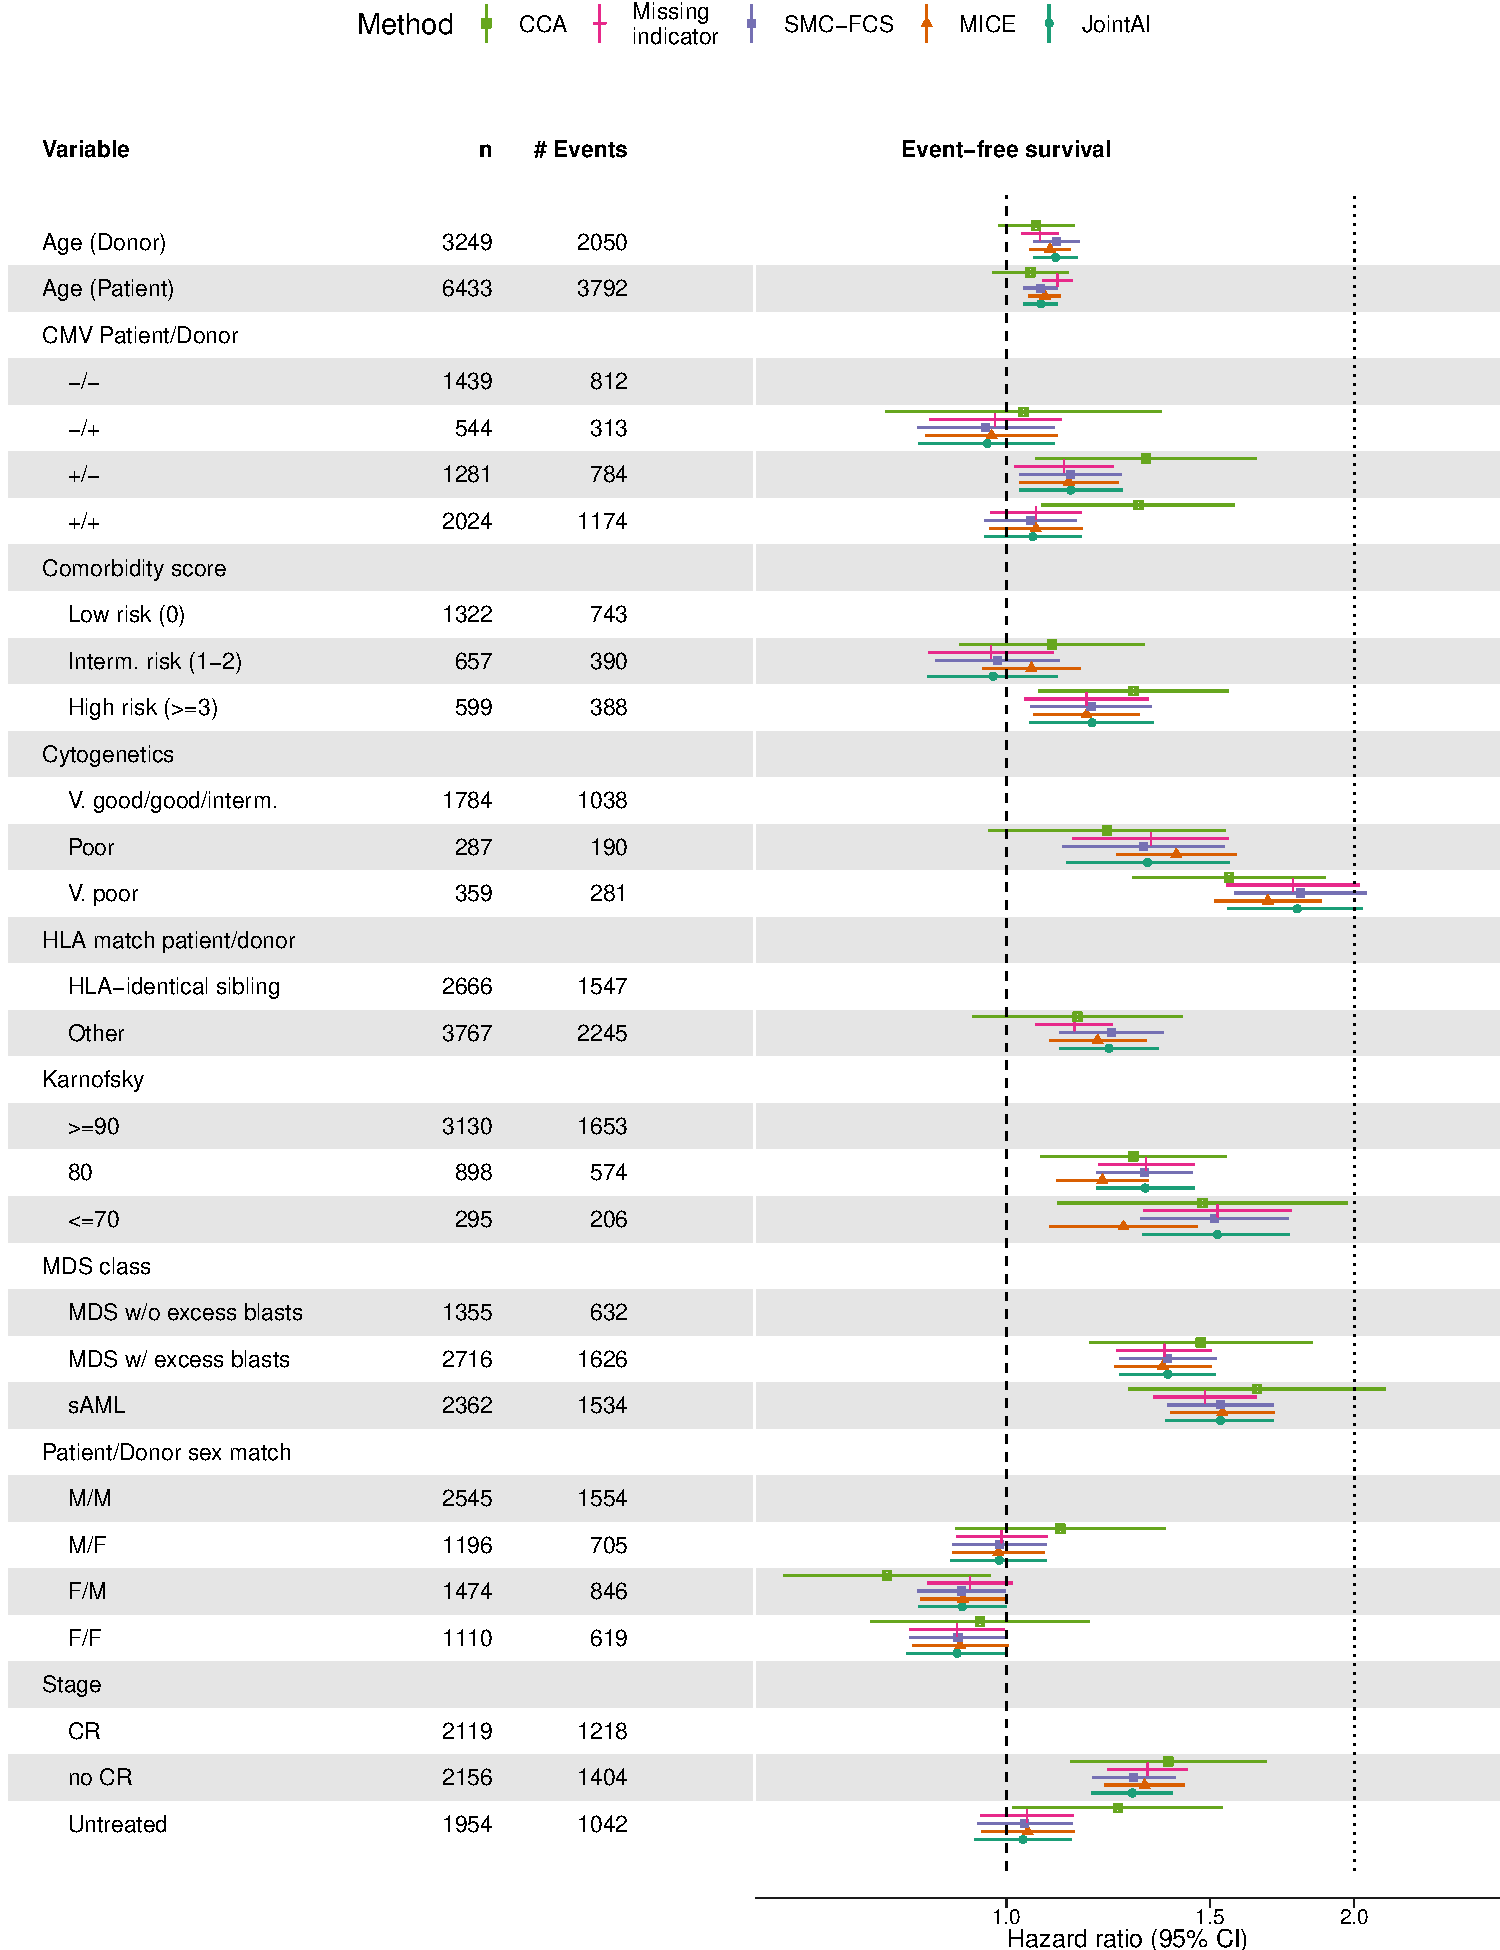
\includegraphics[width=0.85\textwidth,height=\textheight]{chapters/../figures/haema-review_forest-EFS.pdf}

}

\caption{\label{fig-forest-efs}Point estimates and associated 95\%
confidence intervals for the Cox model for relapse-free survival,
according to missing data handling method. Variables and their
descriptions can be found in Table~\ref{tbl-data-dictionary}. Per level
of factor and for continuous variables, we show the observed counts (n)
and the number of events (\# Events, which is the sum of relapse and
non-relapse mortality events) in the full dataset.}

\end{figure}

\hypertarget{discussion-and-recommendations}{%
\section{Discussion and
recommendations}\label{discussion-and-recommendations}}

Our systematic review demonstrated that missing data feature prominently
across studies from major journals in the field of clinical haematology.
Studies are often observational in nature, sometimes making use of large
registries where whether or not a variable is recorded can depend on a
multitude of reasons (e.g.~variables collected only from a certain date,
in particular centers). While presence of missing values was seemingly
consistently reported (usually in the descriptives table), the method
used for dealing with them was not. CCA was the dominant approach to
handling missing values, and the associated loss of efficiency was
generally poorly documented. Importantly, we also note that articles
with seemingly complete data (particularly in observational studies) may
have for simplicity chosen to filter out the missing values at a
pre-processing step, without reporting it in the main manuscript -
implying that the true prevalence of missing data is likely higher than
reported in our review.

Various articles have attempted to raise the bar when it comes to
reporting and handling of missing values more generally across
observational studies. A convenient summary of guidelines found in
(\protect\hyperlink{ref-sterneMultipleImputationMissing2009}{Sterne
\emph{et al.}, 2009},
\protect\hyperlink{ref-sterneROBINSIToolAssessing2016}{2016};
\protect\hyperlink{ref-vandenbrouckeStrengtheningReportingObservational2007}{Vandenbroucke
\emph{et al.}, 2007}) can be found in Table 1 from
(\protect\hyperlink{ref-carrollHowAreMissing2020}{Carroll \emph{et al.},
2020}), and should be considered alongside further guidelines given by
(\protect\hyperlink{ref-leeFrameworkTreatmentReporting2021}{Lee \emph{et
al.}, 2021}). The aforementioned guidelines put findings concerning
missing values reporting in our systematic review into perspective:
while the reporting may have been consistent across articles, it was by
no means thorough. Paz D.L. \emph{et al.}
(\protect\hyperlink{ref-pazd.l.GenomicAnalysisPrimary2021}{2021}) were
perhaps the only standout article from the corpus in this respect. In
their supplemental data, they provided a plot showing the missing data
patterns (i.e.~not only frequencies of missing values per variable, but
also frequencies for two or more variables being simultaneously
missing), and presented a table showing the distribution of variables
among complete cases versus cases with at least one missing value.

The review also showed that while multiple imputation remains an active
topic of methodological research, its application in clinical
haematological studies appears to be very limited. This does seem to
contrast with findings regarding the increasing use of MI in the
\emph{Lancet} and \emph{New England Journal of Medicine} over a period
of 5 years
(\protect\hyperlink{ref-hayatirezvanRiseMultipleImputation2015}{Hayati
Rezvan \emph{et al.}, 2015}).

The systematic review had several strengths. The articles included
covered the main haematological malignancies, as well as a (impact
factor based) large range of journals. In order to obtain as
representative a corpus as possible, we made sure to keep our initial
criteria rather broad: filtering by journals, and by words (in abstract,
title or keywords) directly referring to particular malignancies or
multivariable Cox models. Importantly, we made sure not to include words
such as imputation, missing or incomplete data in this initial search,
as that could severely bias the sample towards articles which were
exceptionally diligent with their missing data reporting.

One of the limitations of the present work is that the articles spanned
a single year, and thereby may not be fully representative of trends in
the literature. Furthermore, the extraction was limited in scope: we did
not record many factors that may be of interest to stratify the results
by, such as study type or goals (e.g.~prediction), as was thoroughly
done for example in Carroll \emph{et al.}
(\protect\hyperlink{ref-carrollHowAreMissing2020}{2020}). We effectively
accepted the trade-off of having a larger sample of articles, in
exchange for limited granularity on the information extraction.

As mentioned previously, extensive guidelines concerning the reporting
and handling of missing values already exist, and are clearly not being
adhered to. Among the few papers using multiple imputation, very little
is reported except the number of imputed datasets: whether it be the
number of iterations, the contents of the imputation model, or the
discussion on the plausibility of the MAR assumption. We argue that at
bare minimum, authors must (in the main article) a) state whether there
were missing values, and if so, across which variables and in what
frequency; b) make explicit whether and how their initial study
population choice has been influenced by missing values; c) explicitly
state the method used for handling the missing values. In the case of a
CCA, one should then clearly report the sample size per analysis model.
Given tight word count limitations for main text of many of the
journals, authors should be encouraged to make use of supplemental
materials to report additional information concerning the missing
values. This may include discussion concerning the reasons why values
were missing, comparison of outcomes between those with and without
missing values, and full details behind the imputation procedure if an
imputation method was used.

The choice of method for handling missing values in covariates will
inevitably be highly context-dependent. For example, while the MIM is
generally discouraged for observational studies
(\protect\hyperlink{ref-groenwoldMissingCovariateData2012}{Groenwold
\emph{et al.}, 2012}), its use has been approved for randomized trials
(\protect\hyperlink{ref-sullivanShouldMultipleImputation2018}{Sullivan
\emph{et al.}, 2018};
\protect\hyperlink{ref-whiteAdjustingPartiallyMissing2005}{White and
Thompson, 2005}). For observational studies, the flowchart shown in
Figure 3 in Lee \emph{et al.}
(\protect\hyperlink{ref-leeFrameworkTreatmentReporting2021}{2021})
provides a solid guide to motivating the choice of method for handling
missing data. We would add that, if the MAR assumption is deemed
plausible, results from a MI procedure (ideally SMC-FCS or fully
Bayesian imputation, at least in the survival analysis context) should
always be presented alongside the results of a CCA. Note that in cases
where there are relatively few missing values, the imputation step could
be skipped entirely: a CCA will likely be efficient enough, and will be
unbiased under (covariate-dependent) MAR. In other cases, particularly
when (auxiliary) variables related to either the variables with missing
values or the mechanism are at the researcher's disposal, MI should be
considered in order to mitigate a potentially important loss of
statistical power. Nevertheless, the proportion of incomplete cases
should not be the main criterion in deciding which method to use: when
the imputation model is well specified and data are MAR, MI can yield
unbiased results even with a large proportion of incomplete cases
(\protect\hyperlink{ref-madley-dowdProportionMissingData2019}{Madley-Dowd
\emph{et al.}, 2019}). Conversely, when either condition is not met
(well specified imputation model and MAR), bias in the results will
likely increase with the proportion of incomplete cases. Additionally,
we caution that there is a lack of research concerning the use of MI for
missing covariates in the presence of multiple outcomes. This is clearly
relevant to articles in clinical haematology, which often present models
for outcomes such as overall survival, relapse of a disease, and
occurrence of graft-versus-host disease (GvHD) as part of a single
study.

In conclusion, missing values are a prominent issue across studies in
clinical haematology, and increased attention should be given in
particular to the methods used to handle them, and the assumptions they
make. In particular, we hope to stimulate a more open discussion about
missingness mechanisms (and their implications on the validity of
analyses), which can encourage better and more complete data collection
in future studies. Nevertheless, researchers should remain prepared to
discuss how the missing values in their particular context could affect
the results of their study, both in terms of bias and statistical power.

\bookmarksetup{startatroot}

\hypertarget{multiple-imputation-for-cause-specific-cox-models-assessing-methods-for-estimation-and-prediction}{%
\chapter{Multiple imputation for cause-specific Cox models: Assessing
methods for estimation and
prediction}\label{multiple-imputation-for-cause-specific-cox-models-assessing-methods-for-estimation-and-prediction}}

In studies analyzing competing time-to-event outcomes, interest often
lies in both estimating the effects of baseline covariates on the
cause-specific hazards, and predicting cumulative incidence functions.
When missing values occur in these baseline covariates, they may be
discarded as part of a complete case analysis (CCA) or multiply imputed.
In the latter case, the imputations may be performed either compatibly
with a substantive model pre-specified as a cause-specific Cox model
(SMC-FCS), or approximately so (MICE). In a large simulation study, we
assessed the performance of these three different methods in terms of
estimating cause-specific regression coefficients and predicting
cumulative incidence functions. Concerning regression coefficients,
results provide further support for use of SMC-FCS over MICE,
particularly when covariate effects are large and the baseline hazards
of the competing events are substantially different. CCA also shows
adequate performance in settings where missingness is not
outcome-dependent. With regard to cumulative incidence prediction,
SMC-FCS and MICE performed more similarly, as also evidenced in the
illustrative analysis of competing outcomes following a hematopoietic
stem cell transplantation. The findings are discussed alongside
recommendations for practising statisticians.

\hfill\break

\hypertarget{introduction-1}{%
\section{Introduction}\label{introduction-1}}

Missing covariate data are of perennial concern in observational studies
in medicine (\protect\hyperlink{ref-carrollHowAreMissing2020}{Carroll
\emph{et al.}, 2020}). The backbone of such studies are clinical
registries, which collect patient data potentially spanning many
countries and centres over long periods of time. These and other data
management complexities can lead to various patterns of (possibly
informative) missingness. Furthermore, these registries are often set up
for multiple purposes leading to multiple studies where different
potentially exclusive survival outcomes could be considered.
Consequently, \emph{competing risks} outcomes are frequently
investigated. This refers to a setting in which individuals can only
experience one of several mutually exclusive events.

In studies considering competing risks outcomes, interest can lie in
both the probabilities of events occurring over time and the effect of
covariates on the different competing events. Appropriate handling of
missing data is then of central concern in view of avoiding potential
bias and/or loss of power when estimating these quantities, as could be
expected when using simple methods such as complete-case analysis (CCA)
(\protect\hyperlink{ref-whiteBiasEfficiencyMultiple2010}{White and
Carlin, 2010}).

A more principled approach to handling missing covariate data is to use
multiple imputation (MI), where a set of complete datasets is generated
using samples based on an imputation model to fill in the missing values
(\protect\hyperlink{ref-murrayMultipleImputationReview2018}{Murray,
2018}). A substantive model is then run on each of these datasets,
before combining the estimates using rules that adequately reflect the
uncertainty in the imputation procedure
(\protect\hyperlink{ref-rubin:1987}{Rubin, 1987}). The imputation model
and the substantive model should ideally be compatible, that is,
deriving from a joint model under which both models are conditionals. If
data are missing across multiple covariates, the fully conditional
specification approach can be used
(\protect\hyperlink{ref-vanbuurenFullyConditionalSpecification2006}{van
Buuren \emph{et al.}, 2006}). This involves specifying an imputation
model for each variable with missing values, fully conditional on the
other variables, including the outcome. The procedure is better known
under its more popular name `multivariate imputation by chained
equations' (MICE)
(\protect\hyperlink{ref-vanbuurens.FlexibleMultivariateImputation1999}{van
Buuren, S. \emph{et al.}, 1999}).

In time-to-event analysis, a popular choice of substantive model is the
Cox proportional hazards model. White and Royston
(\protect\hyperlink{ref-whiteImputingMissingCovariate2009}{2009}) showed
that when using MICE in the context of a Cox model (in absence of
competing events), for each covariate with missing data, the
corresponding imputation model should include the remaining covariates,
the event indicator, and the cumulative baseline hazard. To implement
this model, the cumulative baseline hazard can be approximated by the
marginal Nelson-Aalen estimate of the cumulative hazard. Moreover,
depending on the type of covariate, the imputation model is simplified
with a Taylor approximation for the non-linear terms from the Cox
likelihood. In view of this approximate compatibility between the
substantive and imputation model, Bartlett \emph{et al.}
(\protect\hyperlink{ref-bartlettMultipleImputationCovariates2015}{2015})
proposed a variant of MICE called `substantive model compatible fully
conditional specification' (SMC-FCS). The approach ensures full
compatibility between the imputation model and the substantive model by
imputing missing covariate values in a rejection sampling procedure.

In competing risks settings, where the analysis model of interest is
often a \emph{cause-specific} Cox proportional hazards model, there has
been little research addressing the appropriate use of MI when imputing
missing covariate data
(\protect\hyperlink{ref-lauMissingnessSettingCompeting2018}{Lau and
Lesko, 2018}). The most prominent work is that of Bartlett and Taylor
(\protect\hyperlink{ref-bartlettMissingCovariatesCompeting2016}{2016}),
where the SMC-FCS approach was extended for cause-specific Cox models.
In a simulation study as part of their work, Bartlett and Taylor
compared SMC-FCS to an approximate MICE procedure proposed by
Resche-Rigon \emph{et al.}
(\protect\hyperlink{ref-resche-rigonImputingMissingCovariate2012}{2012}).
The proposal was an extension of the work of White and Royston for
cause-specific Cox models. Simulation results suggested using SMC-FCS
generally leads to estimates with little bias and nominal coverage
(\protect\hyperlink{ref-bartlettMissingCovariatesCompeting2016}{Bartlett
and Taylor, 2016}). In contrast, the approximate MICE approach was often
biased, with some mitigation using interaction terms in the imputation
model.

Importantly, we remark that the algebraic motivation behind the
approximate MICE approach is currently unpublished. Moreover, the work
of Bartlett and Taylor is to our knowledge the only empirical comparison
of this approximate MICE approach with the SMC-FCS approach. Thus,
questions regarding performance of both methods in a wider range of
situations still remain. In addition, the question of how both the
approaches perform with regard to predicted cumulative incidence
functions is hitherto unexplored.

The aim of the present research is thus threefold. First, we aim to
formally extend the work of White and Royston for cause-specific Cox
models. Specifically, we will derive the approximately compatible
imputation models for continuous, binary and multi-level categorical
missing covariates. This extension was originally initiated by one of
the authors of the current manuscript and shared as part of an oral
presentation
(\protect\hyperlink{ref-resche-rigonImputingMissingCovariate2012}{Resche-Rigon
\emph{et al.}, 2012}). Second, we aim to replicate and extend the
simulations of Bartlett and Taylor; additionally manipulating the shape
of the competing baseline hazards and the strength of missingness
mechanisms, among other extensions. Third, we will explore how biases in
cause-specific Cox models affect predicted cumulative incidence
functions for patterns of reference covariate values. Simulation results
will be interpreted alongside an illustrative analysis using a dataset
from the field of allogeneic hematopoietic stem cell transplantation
(alloHCT).

In Section~\ref{sec-motivating-example}, we present the motivating
dataset, and in Section~\ref{sec-comprisks} we introduce notation for
cause-specific competing risks analysis. In
Section~\ref{sec-imp-models}, the algebraic motivation behind the
imputation model for a cause-specific Cox analysis model is shown. The
simulation study is presented in Section~\ref{sec-simstudy}, followed by
an illustrative analysis in Section~\ref{sec-illust-analysis}. Findings
are discussed alongside recommendations for practice in
Section~\ref{sec-cs-MI-discussion}.

\hypertarget{sec-motivating-example}{%
\section{Motivating example}\label{sec-motivating-example}}

Schetelig \emph{et al.}
(\protect\hyperlink{ref-scheteligLateTreatmentrelatedMortality2019}{2019})
assessed long-term outcomes of patients with myelodysplastic syndromes
(MDS) or secondary acute myeloid leukemia (sAML) after an alloHCT. MDS
is characterised by the production of deficient clonal blood cells in
the bone marrow and can rapidly progress to more severe sAML
(\protect\hyperlink{ref-adesMyelodysplasticSyndromes2014}{Adès \emph{et
al.}, 2014}). AlloHCT is the only treatment that can offer long-term
remission of the disease. Therefore, alloHCT is recommended for disease
stages at high risk of transformation into AML or death from other
complications. However, this procedure is associated with a high risk of
adverse outcomes, either due to relapse of MDS or sAML, or due to side
effects of the (pre-)treatment. This leads to the competing risks
outcomes relapse and non-relapse mortality.

The dataset contains 6434 patients transplanted between 2000-2012, and
registered with the EBMT. Several possible predictors measured at time
of transplantation have a substantial amount of missing values. Some
examples of variables with missing values are cytogenetic classification
(62.2\% missing), comorbidity index (59.9\% missing) and the Karnofsky
performance score (32.8\% missing). A cause-specific model for relapse
with the aforementioned three variables as predictors, performed on
complete cases only, makes use of a mere 20\% of the full dataset. The
immediate lack of efficiency here prompted an investigation as to the
performance of MI for such examples.

\hypertarget{sec-comprisks}{%
\section{Cause-specific competing risks analysis}\label{sec-comprisks}}

In a competing risks setting, we assume that individuals can `fail' from
only one of \(K\) distinct events. We denote that failure time as
\(\tilde{T}\), and the competing event indicator as
\(\tilde{D} \in \{1,...,K\}\). In practice, individuals are subject to
some right-censoring time \(C\), which is assumed to be independent of
\(\tilde{T}\) and \(\tilde{D}\), possibly given covariates. We thus only
observe realisations \((t_i, d_i)\) of \(T = \min(C,\tilde{T})\) and
\(D = I(\tilde{T} \leq C)\tilde{D}\), where \(D = 0\) indicates a
right-censored observation.

If we view competing risks as a multi-state process, with a single
(event-free) initial state and \(K\) absorbing states, interest often
lies in the cause-specific hazard, defined for a single event \(k\) as

\begin{equation*}
    h_k(t) = \lim_{\Delta t \to 0} \frac{P(t \leq \tilde{T} < t + \Delta t, \tilde{D} = k \mid \tilde{T} \geq t)}{\Delta t}.
\end{equation*} This hazard function can be interpreted as the
instantaneous force of transition, or intensity, of moving between the
initial state and state \(k\)
(\protect\hyperlink{ref-beyersmannCompetingRisksMultistate2012}{Beyersmann
\emph{et al.}, 2012};
\protect\hyperlink{ref-putterTutorialBiostatisticsCompeting2007}{Putter
\emph{et al.}, 2007}). A model can then be specified, conditional on a
covariate vector \(\mathbf{Z}\). A Cox model is the common choice,
defined for a failure cause \(k\) as

\begin{equation*}
    h_k(t \mid \mathbf{Z}) = h_{k0}(t)\exp(\boldsymbol{\beta}_k^\intercal \mathbf{Z}),
\end{equation*} where \(h_{k0}(t)\) is the cause-specific baseline
hazard, and \(\boldsymbol{\beta}_k\) represents the effects of
covariates \(\mathbf{Z}\) on the cause-specific hazard. We note that in
what follows, we use `effect' to refer to the impact of a covariate in a
multivariable model where there may be non-negligible additional
confounding, and this should hence not be interpreted as a fully causal
quantity. Furthermore, the \(K\) hazard functions define the
failure-free survival probability:

\begin{equation*}
    S(t \mid \mathbf{Z}) = \exp \left( - \sum_{k = 1}^{K} \int_{0}^{t} h_k(u \mid \mathbf{Z})du \right)
        = \exp \left( - \sum_{k = 1}^{K} H_k(t \mid \mathbf{Z}) \right),
\end{equation*} where
\(H_k(t \mid \mathbf{Z}) = \int_{0}^{t} h_k(u \mid \mathbf{Z})du\) is
the cause-specific cumulative hazard for cause \(k\). Assuming
conditional non-informative censoring, the likelihood contribution of an
individual with observations \((t_i, d_i, \mathbf{z}_i)\) is then

\begin{equation}
    \label{eq:likelihood}
    p(t_i, d_i \mid \mathbf{z}_i) = S(t_i \mid \mathbf{z}_i) \prod_{k=1}^{K} \left[ h_k(t_i \mid \mathbf{z}_i) \right]^{I(d_i=k)},
\end{equation} where \(I(\cdot)\) is the indicator function. The
covariate effects \(\boldsymbol{\beta}_k\) on the cause-specific hazard
can then be estimated by optimising the partial likelihood
(\protect\hyperlink{ref-coxPartialLikelihood1975}{Cox, 1975}). This
follows from the observation that the above expression factorises into
separate factors for each cause \(k\), which each corresponding to a
standard Cox likelihood function where events from all other causes are
treated as censored observations
(\protect\hyperlink{ref-prenticeAnalysisFailureTimes1978}{Prentice
\emph{et al.}, 1978}).

\hypertarget{cumulative-incidence-functions}{%
\subsection{Cumulative incidence
functions}\label{cumulative-incidence-functions}}

Beyond assessing covariates, cause-specific hazards can also be used to
estimate the so-called cumulative incidence functions, defined as

\begin{align}
    P(\tilde{T} \leq t, \tilde{D} = k) &= \int_{0}^{t}h_k(u)S(u-)du, \ k=1,...,K,
\end{align} where \(S(u-)\) is the failure-free survival probability
just prior to \(u\)
(\protect\hyperlink{ref-andersenCompetingRisksMultistate2002}{Andersen
\emph{et al.}, 2002}). This cumulative incidence function, or transition
probability, is the probability of experiencing event \(k\) before or at
time \(t\). It is also known as the absolute, or crude risk. It can be
computed either non-parametrically, or semi-parametrically if Cox models
are specified for the \(h_k(u)\). In the latter case, the cumulative
hazards derived from the Breslow estimator of the cumulative
cause-specific baseline hazards are used as ingredients for estimating
the cumulative incidence for cause \(k\).

This implies that we do not need to model the cumulative incidence
function \emph{directly} in order to obtain these predicted
probabilities, as is done when using the Fine--Gray model
(\protect\hyperlink{ref-fineProportionalHazardsModel1999}{Fine and Gray,
1999}). This is helpful given that in observational studies, interest is
seldom in prediction alone: predictions are often presented after first
reporting and interpreting model coefficients. The cause-specific
hazards framework provides a more natural scale on which to interpret
covariate effects, and allows to obtain predicted patient-specific
cumulative incidence functions for all causes.

\hypertarget{sec-imp-models}{%
\section{Methods}\label{sec-imp-models}}

In this section, we provide a framework for using MICE and SMC-FCS for
both estimation of cause-specific regression coefficients, and
cumulative incidence functions. Throughout, we assume that data are
missing according to a missing (completely) at random mechanism,
hereafter abbreviated as M(C)AR.

\hypertarget{sec-imp-models-main}{%
\subsection{Fully conditional approach
(MICE)}\label{sec-imp-models-main}}

We introduce \(X\) as a single, partially observed covariate, and \(Z\)
as a fully observed covariate. We note that \(Z\) could also represent a
vector of complete covariates. Appropriate use of MICE for
cause-specific competing risks analysis requires the specification of an
\emph{imputation model} \(p(X \mid T,D,Z)\), from which a number of
imputed datasets are generated. Detailed derivations for
\(p(X \mid T,D,Z)\) are provided in Appendix A, which we summarise in
the present subsection.

To begin with, we note that by Bayes' Theorem,

\begin{equation}\protect\hypertarget{eq-cond-dist}{}{
    \log p(X \mid T,D,Z) = \log p(T,D \mid X, Z) + \log p(X \mid Z) + c,
}\label{eq-cond-dist}\end{equation} where \(c\) is a constant term that
does not depend on \(X\). For \(p(T,D \mid X, Z)\), a cause-specific Cox
proportional hazards model for each failure cause \(k\) is specified as
\(h_k(t \mid X, Z) = h_{k0}(t)\exp(\beta_k X + \gamma_k Z)\). In case of
binary or continuous \(X\) and \(Z\), \(\beta_k\) and \(\gamma_k\) are
scalars; for categorical \(X\) or \(Z\) with two or more levels,
\(\beta_k\) and \(\gamma_k\) are vectors and \(X\) and \(Z\) represent
dummy codings for the levels of the covariates. To impute from the fully
conditional distribution in Equation~\ref{eq-cond-dist}, we also need to
specify a model for the missing data, \(p(X \mid Z)\). This model will
generally vary depending on the covariate type of \(X\).

\hypertarget{binary-x}{%
\subsubsection{Binary X}\label{binary-x}}

If \(X\) is binary, we could assume
\(\logit P(X = 1 \mid Z) = \zeta_0 + \zeta_1 Z\). If \(Z\) is
categorical with \(J \geq 2\) levels (without loss of generality
assuming that \(Z\) takes values in \(1, \ldots, J\)), we can write

\begin{equation}\protect\hypertarget{eq-Xbin-Zcat}{}{
\begin{aligned}
    \logit P(X = 1 \mid T, D, Z) &= \alpha_0 + \sum^K_{k = 1}\alpha_k I(D=k) + \sum^K_{k = 1} \alpha_{K+k} H_{k0}(T) \nonumber \\
    &\qquad + \sum^{J-1}_{j=1}\alpha_{2K + j}I(Z = j) + \sum^{J-1}_{j=1} \sum^K_{k = 1} \alpha_{(j+1)K + (J-1) + k}I(Z = j) H_{k0}(T),
\end{aligned}
}\label{eq-Xbin-Zcat}\end{equation} which implies that for categorical
\(Z\) we can impute missing \(X\) values using a logistic regression
with \(D\) (as a factor variable), the cumulative baseline hazards for
all causes of failure, \(Z\) (as a factor variable), and the complete
interactions between the cumulative baseline hazards and \(Z\). For
continuous \(Z\), results are no longer exact. Using a first-order
Taylor approximation for the \(\exp(\gamma_k Z)\) term, we can write
\begin{equation}\protect\hypertarget{eq-Xbin-Zcontin}{}{
\begin{aligned}
    \logit P(X = 1 \mid T, D, Z) &\approx \alpha_0  + \sum^K_{k = 1} \alpha_{k} I(D=k) + \sum^K_{k = 1} \alpha_{K + k} H_{k0}(T) + \sum^K_{k = 1} \alpha_{2K + k} H_{k0}(T) Z \nonumber \\
    &\qquad + \alpha_{3K + 1} Z,
\end{aligned}
}\label{eq-Xbin-Zcontin}\end{equation} which is valid if
\(\Var(\gamma_k Z)\) is small. This approximate imputation model thus
uses \(D\), \(Z\), all \(H_{k0}(T)\) and the interactions between all
\(H_{k0}(T)\) and \(Z\) as predictors in a logistic regression. Note
that the \(\alpha\) parameters used above and in the next subsections
represent the imputation model coefficients, and are themselves
functions of other (substantive and missing data model) parameters.
Therefore, these will vary depending on the covariate types of \(X\) and
\(Z\), and the parametrization of the substantive model (i.e.~whether
each cause-specific model has the same predictors, and their functional
forms).

\hypertarget{nominal-categorical-x}{%
\subsubsection{Nominal categorical X}\label{nominal-categorical-x}}

If \(X\) is a categorical covariate with \(J \geq 2\) levels and
\(j = \{0,..., J-1\}\), we can specify different imputation models
depending on whether \(X\) is ordered or not. In the unordered (nominal)
case, we can specify a multinomial logistic regression for
\(p(X \mid Z)\), yielding

\[
\begin{aligned}
    \log \frac{P(X = j \mid T,D,Z)}{P(X = 0\mid T,D,Z)} &\approx \alpha_{j,0}  + \sum^K_{k = 1} \alpha_{j,k} I(D=k) + \sum^K_{k = 1} \alpha_{j,K + k} H_{k0}(T) + \sum^K_{k = 1} \alpha_{j,2K + k} H_{k0}(T) Z \nonumber \\
    &\qquad + \alpha_{j,3K + 1} Z.
\end{aligned}
\] This comes as a result of generalising
\(\logit P(X=1|Z) = \zeta_0 + \zeta_1 Z\) to
\(\log \frac{P(X=j|Z)}{P(X=0|Z)} = \zeta_0 + \zeta_j Z\), and holds for
continuous \(Z\) as in Equation~\ref{eq-Xbin-Zcontin}. For categorical
or no \(Z\), where for the former \(I(Z = j)\) should be used as in
Equation~\ref{eq-Xbin-Zcat}, the expression for the fully conditional
distribution is exact as in the binary case. The predictors to be
included in the imputation model are exactly the same as for binary
\(X\).

\hypertarget{ordered-categorical-x}{%
\subsubsection{Ordered categorical X}\label{ordered-categorical-x}}

For ordered categorical \(X\), a proportional odds model could be
assumed as \(\logit P(X \leq j \mid Z) = \zeta_{j} + \zeta_Z Z\). This
however implies that the fully conditional distribution requires
specifying \(p(T,D \mid X \leq j, Z)\), which does not have a standard
proportional hazards density. Instead, it has a \emph{weighted sum} of
proportional hazards densities. Thus, the expression for
\(P(X \leq j \mid T, D, Z)\) does not extend from the binary case in any
simple form. Nevertheless, a proportional odds model including \(D\),
\(Z\) and all \(H_{k0}(T)\) could still be used to impute the missing
\(X\) values, though the properties of such a model are not currently
well known. We refer the reader to the book written by McCullagh and
Nelder (\protect\hyperlink{ref-mccullagh1989generalized}{1989}) for a
detailed description of both the multinomial logistic regression and
proportional odds models.

\hypertarget{continuous-x}{%
\subsubsection{Continuous X}\label{continuous-x}}

If \(X\) is a continuous covariate, we could assume it to be normal
conditional on \(Z\) (possibly after transformation), as
\(X \mid Z \sim \mathcal{N}(\zeta_0 + \zeta_1 Z, \sigma^2)\). The
implied expression for \(p(X \mid T, D, Z)\) is not normal due to the
\(\exp(\beta_k X + \gamma_k Z)\) term, and so a bivariate Taylor
approximation is used around the sample means \(\bar{X}\) and
\(\bar{Z}\). To the first degree, the approximate fully conditional
distribution is expressed as

\begin{equation*}
    X \mid T, D, Z \sim \mathcal{N}(\alpha_0 + \alpha_1 Z + \sum^K_{k = 1} \alpha_{k+1} I(D=k) + \sum^K_{k = 1} \alpha_{K + k + 1} H_{k0}(T),\sigma^2).
\end{equation*} This suggests a model for imputing continuous \(X\)
should be a linear regression with \(D\), \(Z\) and all \(H_{k0}(T)\)
again as predictors. With a quadratic approximation for
\(\exp(\beta_k X + \gamma_k Z)\), the accuracy of the above model can be
improved by additionally including the interactions between all
\(H_{k0}(T)\) and \(Z\). The approximations are valid under the
assumption of small \(\Var(\beta_k X + \gamma_k Z)\).

We note that the above models, like in the simple time-to-event
settings, cannot be implemented without a working estimate of
\(H_{k0}(T)\) - whose true values we will assume are unknown. For the
competing risks setting, we can use the marginal Nelson-Aalen estimate
of the cumulative cause-specific hazard (which requires treating all
events other than \(k\) as censored) as an approximation for
\(H_{k0}(T)\). As explained by White and Royston
(\protect\hyperlink{ref-whiteImputingMissingCovariate2009}{2009}), this
approximation becomes poorer with larger true covariate effects. We may
then expect the estimated covariate effects after the imputation
procedure to be biased.

\hypertarget{sec-smcfcs-theory}{%
\subsection{Substantive model compatible
approach}\label{sec-smcfcs-theory}}

We refer the reader to the work of Bartlett \emph{et al.}
(\protect\hyperlink{ref-bartlettMultipleImputationCovariates2015}{2015})
for a detailed introduction of the SMC-FCS method, and to the work of
Bartlett and Taylor
(\protect\hyperlink{ref-bartlettMissingCovariatesCompeting2016}{2016})
for its specific extension to cause-specific Cox proportional hazards
models. Briefly, the SMC-FCS method (in the current setting) is based on
application of Bayes' theorem,

\begin{equation}\protect\hypertarget{eq-smcfcs-propdens}{}{
  p(X \mid T, D, Z) \propto p(T,D \mid X, Z)p(X \mid Z),
}\label{eq-smcfcs-propdens}\end{equation} which was already introduced
on the logarithmic scale in Equation~\ref{eq-cond-dist}. The parameters
associated with both \(p(T,D \mid X, Z)\) and \(p(X \mid Z)\) are
omitted for readability. In essence, the procedure involves choosing
\(p(X \mid Z)\) as a proposal density and using rejection sampling to
draw possible values for missing \(X\) from a density proportional to
\(p(T,D \mid X, Z)p(X \mid Z)\). This is under the assumption that
\(p(X \mid Z)\) is simple to sample from, as is the case if we specify a
model for it, e.g.~a linear regression of \(X\) conditional on \(Z\).
The imputation model is then compatible with the substantive model in
the sense that a joint distribution exists which contains both the
substantive model and the imputation model as its conditional
distributions. If multiple covariates have missing data, it is still
possible to specify mutually incompatible models for \(p(X \mid Z)\),
but each fully conditional distribution will be compatible with the
substantive model.

In contrast to MICE, the SMC-FCS approach does not require any
approximations - neither for the non-linear terms, nor for the
cumulative baseline hazard. Of course, the cumulative baseline hazard
still needs to be evaluated in order to draw from
Equation~\ref{eq-smcfcs-propdens}. In order to do so, the Breslow
estimate is used, and is updated at each iteration of the imputation
procedure conditional on the most recent draws from the posterior
distribution of the regression coefficients.

\hypertarget{regression-coefficients}{%
\subsection{Regression coefficients}\label{regression-coefficients}}

Both the MICE and SMC-FCS procedures result in \(m = 1,...,M\) imputed
datasets. In each of these datasets, the cause-specific Cox model for
one or more of the \(K\) causes of failure is fitted. Let \(\theta\)
denote a cause-specific regression coefficient of interest, and let
\(\hat{\theta}_m\) and \(\widehat{\Var}(\hat{\theta}_m)\) respectively
denote the estimate and associated variance of this coefficient in the
\(m^\textsuperscript{th}\) imputed dataset. We can combine these \(M\)
estimates using Rubin's rules, with estimator

\begin{equation*}
    \hat{\theta} = \frac{1}{M}\sum_{m=1}^{M}\hat{\theta}_m.
\end{equation*} The associated variance estimator is

\begin{equation*}
    \widehat{\Var}(\hat{\theta}) = \frac{1}{M}\sum_{m=1}^{M}\widehat{\Var}(\hat{\theta}_m) + \big(1 + \frac{1}{M}\big)\frac{1}{M-1}\sum_{m=1}^{M}(\hat{\theta}_m - \hat{\theta})^2,
\end{equation*} which combines estimates of within and between
imputation variance (\protect\hyperlink{ref-rubin:1987}{Rubin, 1987}).
The estimate of the standard error is then readily obtained as
\(\widehat{\SE}(\hat{\theta}) = \sqrt{\widehat{\Var}(\hat{\theta})}\).

\hypertarget{predicted-probabilities}{%
\subsection{Predicted probabilities}\label{predicted-probabilities}}

To obtain the predicted cumulative incidence functions for an individual
with fully observed covariates after an MI procedure, there are at least
two possible options. The first is to pool the regression coefficients
and baseline hazards separately, and use those to produce a single
predicted curve. The second approach is to use the substantive models
fitted in each imputed dataset to create \emph{imputation-specific}
predictions, and then pool those (possibly after transformation) using
Rubin's rules. The articles by Wood \emph{et al.}
(\protect\hyperlink{ref-woodEstimationUsePredictions2015}{2015}) and
Mertens \emph{et al.}
(\protect\hyperlink{ref-mertensConstructionAssessmentPrediction2020}{2020})
recommend the second approach, which is the one we employ in the present
paper.

\hypertarget{sec-simstudy}{%
\section{Simulation study}\label{sec-simstudy}}

We designed a simulation study with the aim of comparing the performance
of CCA, MICE and SMC-FCS in the presence of missing baseline covariate
values for cause-specific Cox proportional hazards models with two
competing events. We assessed performance with respect to estimated
regression coefficients, and predicted cumulative incidence functions.

\hypertarget{data-generating-mechanisms}{%
\subsection{Data-generating
mechanisms}\label{data-generating-mechanisms}}

We generated datasets containing \(n = 2000\) individuals, with one
record each containing both predictor and outcome information.

\hypertarget{covariates}{%
\subsubsection{Covariates}\label{covariates}}

Two covariates \(X\) and \(Z\) were generated in each dataset. We varied
the covariate type of \(X\) as either continuous or binary, and \(Z\)
was fixed as continuous. When both covariates were continuous, they were
generated from a bivariate standard normal distribution
\(X,Z \sim \mathcal{N}(\boldsymbol{\mu}, \boldsymbol{\Sigma})\), with
means \(\boldsymbol{\mu} = \{0, 0\}\), variances
\(\text{diag}(\boldsymbol{\Sigma}) = \{1, 1\}\) and correlation
\(\rho = 0.5\).

When \(X\) was binary, we assumed \(X \sim \text{Bern}(0.5)\) and
\(Z \sim N(0, 1)\), with a \emph{point-biserial} correlation between the
two variables of \(\rho = 0.5\). We can generate observations in this
way by first generating \(X'\) and \(Z\) from a bivariate standard
normal distribution with correlation \(\rho' \approx 0.63\), and then
dichotomising \(X'\) at 0 (the value of the standard normal quantile
function for a probability of 0.5) to produce \(X\). We refer the reader
to the work of Demirtas and Hedeker
(\protect\hyperlink{ref-demirtasComputingPointbiserialCorrelation2016}{2016})
for a description of this well-established procedure.

\hypertarget{competing-event-times}{%
\subsubsection{Competing event times}\label{competing-event-times}}

We based our simulation of event times on the motivating alloHCT example
described in Section~\ref{sec-motivating-example}, focusing on the two
competing events relapse (REL) and non-relapse mortality (NRM) over a
10-year follow-up period. To generate the failure times for the
competing events, we made use of latent failure times, denoted \(T_1\)
and \(T_2\) for REL and NRM respectively
(\protect\hyperlink{ref-beyersmannSimulatingCompetingRisks2009}{Beyersmann
\emph{et al.}, 2009}).

Typically in alloHCT studies, patients are at very high risk of both
relapse and NRM in the initial period after alloHCT, with this risk
gradually decreasing thereafter as they survive longer. For this reason,
generating failure times from a distribution with a decreasing hazard
function is appropriate. The Weibull distribution, with probability
density function
\(f(t) = \kappa \lambda t^{\kappa - 1} \exp (-\lambda t^{\kappa})\),
with shape \(\kappa > 0\) and rate \(\lambda > 0\), accommodates
decreasing hazards for \(\kappa < 1\). This is the parametrisation used
in the text by Klein and Moeschberger
(\protect\hyperlink{ref-kleinSurvivalAnalysisTechniques2006}{2003}).

We thus generated both latent failure times from independent Weibull
distributions, assuming cause-specific proportional hazards conditional
on \(X\) and \(Z\). We furthermore generated independent censoring times
from an Exponential distribution. In summary:

\begin{align*}
    \tilde{T}_1 &\sim \text{Weibull}(\kappa_1, \lambda_1 = \lambda_{10}e^{\beta_1 X + \gamma_1 Z}), \\
    \tilde{T}_2 &\sim \text{Weibull}(\kappa_2, \lambda_2 = \lambda_{20}e^{\beta_2 X + \gamma_2 Z}), \\
    C &\sim \text{Exp}(\lambda_C),
\end{align*} where \(\lambda_C\) is the censoring rate, and
\(\lambda_{10}\) and \(\lambda_{20}\) are the baseline hazard rates for
REL and NRM respectively. We then defined
\(\tilde{T} = \text{min}(\tilde{T}_1, \tilde{T}_2)\), with an associated
factor variable \(\tilde{D}\), where \(\tilde{D} =1\) if REL occured
first, and \(\tilde{D} = 2\) otherwise. The generated observed (event or
censoring) time was then defined as \(T = \text{min}(C, \tilde{T})\),
with corresponding indicator \(D = I(\tilde{T} \leq C)\tilde{D}\).

We used estimates from cause-specific marginal accelerated failure time
(AFT) models on the motivating dataset to fix the parameters values of
the baseline shape and hazard rates for the latent failure times.
Weibull AFT models for both causes of failure led to fixing
\(\kappa_1 = 0.58\), \(\lambda_{10} = 0.19\), \(\kappa_2 = 0.53\), and
\(\lambda_{20} = 0.21\). An exponential AFT model for the censoring
distribution motivated setting \(\lambda_C = 0.14\). Since the baseline
hazards for both competing events were estimated to be very similar, we
decide to also vary \(\{\kappa_1,\lambda_{10}\} = \{1.5,0.04\}\), such
that REL had a steadily increasing hazard. Both these `similar' and
`different' baseline hazard configurations lead to comparable marginal
10-year cumulative incidences of both events, in the 35-45\% range.
Regarding cause-specific regression coefficients, we varied
\(\beta_1 = \{0, 0.5, 1\}\), and fixed \(\gamma_1 = 1\),
\(\beta_2 = 0.5\) and \(\gamma_2 = 0.5\).

\hypertarget{missing-data-mechanisms}{%
\subsubsection{Missing data mechanisms}\label{missing-data-mechanisms}}

\(Z\) was conserved as a complete covariate, and missingness was induced
in \(X\). Let \(R_X\) indicate whether elements of \(X\) were missing
(\(R_X = 0\)) or observed (\(R_X = 1\)). We varied the proportion of
missing values as either `low' with 10\% missing, or `high' with 50\%.
We defined four separate missingness mechanisms:

\begin{enumerate}
\def\labelenumi{\arabic{enumi}.}
\item
  Missing completely at random (MCAR), defined as \(P(R_X = 0) = 0.5\)
  or \(P(R_X = 0) = 0.1\).
\item
  Missing at random conditional on \(Z\) (MAR), which was defined as
  \(\logit P(R_X = 0 \mid Z) = \eta_0 + \eta_1 Z\).
\item
  Outcome-dependent missing at random (MAR-T), which was defined as
  \(\logit P(R_X = 0 \mid T_{\text{stand}}) = \eta_0 + \eta_1 T_{\text{stand}}\).
  \(T_{\text{stand}}\) is \(\log T\), standardised to have zero mean and
  unit variance. Note that \(T\) was the observed (event or censoring)
  time; if missingness depended on the true event time, this would lead
  to a missing not at random mechanism.
\item
  Missing not at random conditional on \(X\) (MNAR), which was defined
  as \(\logit P(R_X = 0 \mid X) = \eta_0 + \eta_1 X\).
\end{enumerate}

For mechanisms 2-4, \(\eta_1\) represented the strength and direction of
the missingness mechanism. For example, if \(\eta_1 < 0\) in the MAR
mechanism, observations with smaller values of the \(Z\) had a larger
probability (increasing with more extreme \(\eta_1\)) of the
corresponding \(X\) being missing. In the present study, we varied
\(\eta_1 = \{-1, -2\}\), representing `weak' and `strong' mechanisms
respectively. In this context, the MAR-T mechanism could reflect a
measurement that is only collected if a subject survives long enough
into a study and is in follow-up, as may be the case with a genetic
test. Although this kind of measurement is collected or only available
at a later point in time, it can still be considered as baseline
information and does \emph{not} constitute conditioning on the future.

The value of \(\eta_0\) was chosen (in each simulated dataset) such that
the average missingness probability was equal to either 0.5 or 0.1. This
was done via standard root-solving for a fixed value of \(\eta_1\).

\hypertarget{design}{%
\subsubsection{Design}\label{design}}

The simulation study is chosen to follow a partially factorial design,
where the parameters outlined above are varied systematically. A full
factorial design would result in 4 (missingness mechanisms) \(\times\) 2
(mechanism strengths) \(\times\) 2 (proportions missing data) \(\times\)
2 (covariate types for \(X\)) \(\times\) 2 (baseline hazard
parametrizations) \(\times\) 2 (effects magnitudes of \(X\) on
cause-specific hazard of REL) \(= 128\) scenarios. However, the strength
of the missingness mechanism cannot be varied for MCAR settings by
definition, leaving \(112\) scenarios in total.

\hypertarget{estimands}{%
\subsection{Estimands}\label{estimands}}

The analysis models of interest are the cause-specific Cox proportional
hazards models for REL and NRM,
\(h_k(t \mid X, Z) = h_{k0}(t)\exp(\beta_k X + \gamma_k Z)\) for
\(k = \{1,2\}\). We then have two main sets of estimands of interest:

\begin{itemize}
\item
  \(\theta_{\text{regr}} = \{\beta_1,\gamma_1,\beta_2,\gamma_2\}\),
  which are the data-generating regression coefficients from both
  cause-specific Cox models.
\item
  \(\theta_{\text{pred}}\), which is a vector containing the REL and NRM
  probabilities (cumulative incidences) for a set of reference patients
  at 6 months, 5 years and 10 years after baseline.
\end{itemize}

These reference patients were defined by all combinations of
\(Z_{\text{ref}} = \{-1,0,1\}\) with \(X_{\text{ref}} = \{-1,0,1\}\) for
continuous \(X\), and \(X_{\text{ref}} = \{0,1\}\) for binary \(X\).
Since the data-generating coefficients for both competing events had a
positive effect on the cause-specific hazards, one could for example
refer to \(\{X_{\text{ref}},Z_{\text{ref}}\} = \{1, 1\}\) as a `high
risk' individual, and `low risk' for \(\{-1, -1\}\).

\hypertarget{methods}{%
\subsection{Methods}\label{methods}}

Five missing data methods were compared in each simulation scenario:

\begin{itemize}
\item
  \(CC\) - an analysis run on a dataset after listwise deletion.
\item
  \(CH_{1}\) - MI with imputation model predictors including \(Z\), the
  event indicator solely for event one i.e.~\(I(D = 1)\), and the
  cumulative hazard for REL \(\hat{H}_{1}(T)\) (at the end of follow-up
  for each individual), based on the Nelson-Aalen estimator, as an
  approximation of the cumulative baseline hazard \(\hat{H}_{10}(T)\).
\item
  \(CH_{12}\) - MI with imputation model predictors including \(Z\), the
  event indicator \(D\) as a three level factor variable, and the
  cumulative hazards for both events \(\hat{H}_{1}(T)\) and
  \(\hat{H}_{2}(T)\); outlined in Section~\ref{sec-imp-models-main}.
\item
  \(CH_{12,\text{Int}}\) - identical to the \(CH_{12}\), with the
  addition of the interactions \(\hat{H}_{1}(T) \times Z\) and
  \(\hat{H}_{2}(T) \times Z\); outlined in
  Section~\ref{sec-imp-models-main}.
\item
  smcfcs - the approach outlined in Section~\ref{sec-smcfcs-theory}\},
  using \(Z\) as sole predictor in the \(X \mid Z\) model (default
  setting).
\end{itemize}

The \(CH_{1}\) method corresponds to the `FCS survival' method explored
in the simulation study by Bartlett and Taylor, where failures other
than cause one are treated as censored and the cumulative hazard of
cause two is omitted from the imputation model. It corresponds to a
direct application of the White and Royston
(\protect\hyperlink{ref-whiteImputingMissingCovariate2009}{2009})
results to the cause-specific Cox model for cause one, which may present
itself as intuitive when interest lies in a single failure cause.

Additionally, the model was also fitted on the complete dataset prior to
any missingness being induced in \(X\). For the imputation methods, the
number of imputed datasets was varied as \(m = \{5, 10, 25, 50\}\). We
set \(\max(m) = 50\) since no substantial reduction in empirical
standard errors was observed over trial runs with \(m = 100\). We also
note that for \(m \neq 50\), the imputations were not re-run
independently. Results were instead pooled across the first 5, 10 or 25
imputed datasets from the original 50.

When \(X\) was continuous, the imputation model was a linear regression.
For binary \(X\), the imputation model was a logistic regression. We
note that since there was only one partially observed covariate, chained
equations were not needed. Nevertheless, we still refer to methods
\(CH_{1}\), \(CH_{12}\) and \(CH_{12,\text{Int}}\) under the general
umbrella term `MICE' methods when reporting the results.

\hypertarget{performance-measures}{%
\subsection{Performance measures}\label{performance-measures}}

For \(\theta_{\text{regr}}\), we recorded the point estimates, empirical
and estimated standard errors, absolute bias and coverage probabilities.
As our primary measure of interest was bias, we based the number of
simulation replications per scenario \(n_{\text{sim}}\) on a desired
Monte-Carlo standard error (MCSE) of bias. As per Morris \emph{et al.}
(\protect\hyperlink{ref-morrisUsingSimulationStudies2019}{2019}) this is
defined as
\(\text{MCSE(Bias)} = \sqrt{\Var(\hat{\theta}_{\text{regr}})/n_{\text{sim}}}\).
We assumed that \(\text{SD}(\hat{\theta}_{\text{regr}})\leq 0.125\)
(largest empirical standard error to be expected with binary \(X\),
based on small trial run), and we deemed a
\(\text{MCSE(Bias)} \leq 0.01\) to be appropriate. We thus required
\(n_{\text{sim}} = 0.125^2 / 0.01^2 \approx 156\) replications per
scenario, which we rounded up to \(n_{\text{sim}} = 160\). We thus
generated 160 independent datasets per simulation scenario.

For \(\hat{\theta}_{\text{pred}}\), we recorded the point estimates,
empirical standard errors, absolute bias, coverage probabilities and
root mean square error (RMSE). We focus primarily on reporting bias and
RMSE. Based on trial runs, we assumed
\(\text{SD}(\hat{\theta}_{\text{pred}})\leq 0.05\), which for 160
replications would result in a
\(\text{MCSE(Bias)} \leq 0.05 / \sqrt{160} \approx 0.004\). We thus
proceeded with the same number of simulated datasets.

\hypertarget{software}{%
\subsection{Software}\label{software}}

All analyses were performed using R version 3.6.2
(\protect\hyperlink{ref-rcoreteamLanguageEnvironmentStatistical2020}{R
Core Team, 2020}). The substantive model compatible imputation was
performed using the smcfcs package version 1.4.1
(\protect\hyperlink{ref-bartlettSmcfcsMultipleImputation2022}{Bartlett
\emph{et al.}, 2022}) and MICE was performed using the mice package
version 3.8.0
(\protect\hyperlink{ref-buurenMiceMultivariateImputation2011}{Buuren and
Groothuis-Oudshoorn, 2011}). The cause-specific Cox models were run and
subsequent predicted cumulative incidences were obtained using the
mstate package version 0.2.12
(\protect\hyperlink{ref-dewreedeMstatePackageAnalysis2011}{de Wreede
\emph{et al.}, 2011}).

\hypertarget{results-1}{%
\subsection{Results}\label{results-1}}

We focus primarily on \(\beta_1\) (the regression coefficient for \(X\)
in the cause-specific REL model) and the 5-year probabilities of REL and
NRM. For the imputation methods, we present results only with
\(m = 50\). Full results are reported in the supplementary materials,
linked at the end of the present text.

\hypertarget{regression-coefficients-1}{%
\subsubsection{Regression
coefficients}\label{regression-coefficients-1}}

Figure fig:beta1\_MAR summarises the results with regard to bias in the
estimation of \(\beta_1\) with a MAR mechanism induced on continuous
\(X\). The plot is a variant of a nested-loop plot, where each
colour-cluster of points represents a scenario defined by the step
functions at the bottom of the plot
(\protect\hyperlink{ref-ruckerPresentingSimulationResults2014}{Rücker
and Schwarzer, 2014}). For example, the left-most bin in the plot
corresponds to a scenario with data-generating \(\beta_1 = 0.5\), 10\%
missing data, similar hazard shapes and a weak missingness mechanism.
For readability, the \(CH_{1}\) method and the analysis ran on the full
dataset prior to inducing missing data are omitted from the figure.

First, we note that in the 16 scenarios depicted, both \(CC\) and smcfcs
showed little to no bias in the estimation of \(\beta_1\). For \(CC\),
no bias was expected given that this was a case of covariate-dependent
MAR, and results for smcfcs were in line with the simulations of
Bartlett and Taylor
(\protect\hyperlink{ref-bartlettMissingCovariatesCompeting2016}{2016}).
Second, the MICE methods showed varying amounts of bias depending on the
scenario. With increasing true covariate effects, and higher proportion
of missing values, the bias was larger. This was to be expected in light
of the approximations employed in Section~\ref{sec-imp-models-main},
which are valid for small covariate effects. Moreover, the magnitude of
the bias was also larger when the baseline hazard shapes were different.
Last, adding the interaction terms in the imputation model did not
significantly reduce bias, except when the missingness mechanism was
weak, and the baseline hazard shapes were different.

For contrast, we also present the results for \(\beta_1\) with a MAR-T
mechanism in Figure fig:beta1\_MART, again with continuous \(X\). In
this case, \(CC\) was consistently biased, as is expected when
missingness is dependent on the outcome. Particularly for a high
proportion of missing values, the bias in both MICE methods was even
more severe than that of \(CC\), reaching close to 20\% (relatively).
Conversely, smcfcs was consistently unbiased across the depicted
scenarios.

We also briefly summarise some of the more general findings across the
simulations reported in the supplementary material. First, efficiency
gains (in the form of smaller estimated standard errors) were mainly
observed for \(\gamma_1\) and \(\gamma_2\). Second, the \(CH_{1}\)
method yielded the largest biases, and lowest coverage probabilities of
all methods. This was unsurprising, as \(CH_{1}\) corresponded to
imputing \(X\) as if competing outcomes were considered as censoring.
Third, the findings with MCAR missingness were largely analogous to
those of the MAR reported above; and in presence of MNAR, all imputation
methods (including smcfcs) showed appreciable bias. Last, in scenarios
with binary \(X\), the overall bias in the MICE methods was lower with
respect to scenarios with continuous \(X\). This could be attributed to
the different terms that are being approximated in the imputation
models. In addition to the cumulative baseline hazards, only
\(\exp(\gamma_k Z)\) is being approximated in the case of binary \(X\),
whereas in the continuous case a fuller \(\exp(\beta_k X + \gamma_k Z)\)
is being approximated.

In terms of RMSE, which summarises both bias and variance, the
differences in performance between the methods in M(C)AR scenarios was
smaller, aside from when missingness was high and the baseline hazard
shapes were different (see for example figure 2.1.2 of supplementary
material on regression coefficients).

\hypertarget{predicted-probabilities-1}{%
\subsubsection{Predicted
probabilities}\label{predicted-probabilities-1}}

Concerning predicted probabilities, we focus on the estimation of 5-year
REL and NRM probabilities for a `low-risk' individual,
i.e.~\(\{X,Z\} = \{-1, -1\}\) with continuous \(X\). Figure
fig:5year\_MAR summarises the RMSE of these probabilities under a MAR
mechanism where 50\% of values are missing.

We point the reader to the \(y\)-axis of the plot, where results are now
on the probability scale. The largest RMSE reported in the plot was just
under 2.5\%, with most RMSE values for the imputation methods being
under 1.5\%, with little to no difference between them. In these
scenarios, the imputation methods outperform \(CC\), but with the finest
of margins. This is part of a general finding across the simulations:
the predicted probabilities when using the imputation methods overall
had very little bias, and little reduction in variability was observed
beyond \(m = 25\) imputations. We note that since all methods were
similarly biased under M(C)AR (as seen for example in figure 1.2.1 of
supplementary material on predictions), the RMSE for \(CC\) is expected
to be a factor of \(\sqrt{2}\) larger than for the imputation methods
when missingness was `high', given that \(CC\) used half as much data.

We propose various explanations for this behaviour. First, we note that
the prediction results for \(\{X,Z\} = \{0, 0\}\) (with \(X\) continuous
or binary) can be taken as a proxy for how precisely the cause-specific
baseline hazards are estimated. For all non-MNAR scenarios, little to no
bias was found in the predicted probabilities for these reference
patients. This may be additionally linked to the fact that \(X\) and
\(Z\) are centered and normal, which could imply that
\(H_{k0}(\tilde{T})\) is adequately approximated by the Nelson-Aalen
estimator. Second, regarding regression coefficients, bias was primarily
observed in \(\beta_1\) and \(\beta_2\), with the former showing more
extreme bias when data-generating \(\beta_1 = 1\). Estimates of
\(\gamma_1\) and \(\gamma_2\) however generally only exhibited biases of
up to 5\% in the MAR scenarios, and slightly higher for \(CC\) in MAR-T
scenarios. Well-estimated cause-specific baseline hazards in tandem with
close to unbiased estimates of \(\gamma_k\) could then explain the small
bias in the predictions, since bias in the linear predictor as a whole
(\(\beta_k X + \gamma_k Z\)) only reached 10\% in the most extreme
cases, and was mostly below the 5\% mark otherwise.

\hypertarget{additional-simulations}{%
\subsubsection{Additional simulations}\label{additional-simulations}}

In supplementary material I (available online), we performed two
additional simulation studies. The first investigated the use of the
Breslow estimates of the cumulative baseline hazards in the imputation
model, updated at each iteration of the imputation procedure. Consistent
with earlier results in the standard survival setting, MICE using
intra-iteration updates of the Breslow estimates performed no better
than using the marginal cumulative hazards in the imputation model
(\protect\hyperlink{ref-whiteImputingMissingCovariate2009}{White and
Royston, 2009}). The second study assessed the performance of the MI
methods in the presence of \(K = 3\) competing events. In this setting,
SMC-FCS remained unbiased, while the MICE methods including additional
interaction terms performed slightly better than those without.

\hypertarget{sec-illust-analysis}{%
\section{Illustrative analysis}\label{sec-illust-analysis}}

We used the motivating alloHCT dataset introduced in
Section~\ref{sec-motivating-example} to illustrate the methods described
in the simulation study. Cause-specific Cox proportional hazards models
were fitted for both REL and NRM, conditional on a set of baseline
predictors chosen on the basis of substantive clinical knowledge. An
overview of these predictors, including their names, descriptions and
proportion of missing values, can be found in Appendix B. The same
predictors were used in the models for REL and NRM.

We used the \(CC\), \(CH_{12}\) and smcfcs methods to handle the missing
baseline covariate data, which we assumed to be missing at random. Given
that \(CH_{12,\text{Int}}\) did not show much improvement over
\(CH_{12}\) in the simulation study, we decided to use the more
parsimonious latter. Therefore, the imputation model for a partially
observed covariate using \(CH_{12}\) contained as predictors the
remaining fully and partially observed covariates from the substantive
model, and the marginal cumulative hazards for both events. For smcfcs,
the imputation model similarly contained the remaining fully and
partially observed covariates from the substantive model, which is the
default setting. Continuous covariates were imputed using linear
regression, binary covariates using logistic regression, ordered
categorical using proportional odds regression and nominal categorical
using multinomial logistic regression. Since missingness spanned
multiple covariates, chained equations were required.

To motivate the choice of \(m\) for \(CH_{12}\) and smcfcs, we used von
Hippel's quadratic rule based on the fraction of missing information
(FMI) rather than the proportion of complete cases
(\protect\hyperlink{ref-madley-dowdProportionMissingData2019}{Madley-Dowd
\emph{et al.}, 2019};
\protect\hyperlink{ref-vonhippelHowManyImputations2020}{von Hippel,
2020}). We first ran a set of \(m = 20\) imputations, with
\(n_{\text{iter}} = 20\) iterations. After pooling, the coefficient with
largest FMI was that of donor age in the model for NRM, with a value of
approximately 0.49. Based on an 95\% upper-bound for this FMI, and for a
desired coefficient of variation (CV) of 0.05, we would require
approximately \(m = 84\) imputed datasets. We rounded this upwards, and
performed our final analysis with \(m = 100\). We conserved
\(n_{\text{iter}} = 20\) as convergence was generally observed from 10
iterations onwards.

Figure fig:forest\_mds summarises the exponentiated point estimates
(hazard ratios, HR) and associated 95\% confidence intervals (CI) from
the cause-specific model for REL. The CIs for \(CH_{12}\) and smcfcs are
based on the pooled standard errors and the \(t\)-distribution. First,
we observed a clear gain in efficiency across all coefficients for both
imputation methods relative to \(CC\). Second, there was general
agreement between the estimates obtained from both \(CH_{12}\) and
smcfcs; a finding which was also reported in the illustrative analysis
in the work by Bartlett and Taylor
(\protect\hyperlink{ref-bartlettMissingCovariatesCompeting2016}{2016}).
Third, we did note some differences between \(CC\) and the imputation
methods for certain variables, such as remission status or Karnofsky
score. The most surprising case of this was with the MDS class of the
patient, which was completely observed. In the model for REL, the HR for
the sAML category estimated with \(CC\) is just above three, whereas the
imputation methods estimate it much closer to two. This also raises the
point that for categorical variables, differences in methods can be seen
on the category level rather than on the variable level as a whole - as
also evidenced by the estimated HRs for the cytogenetics variable.
Results for the cause-specific NRM model are summarized in Figure
fig:forest\_nrm.

Furthermore, we computed the predicted 5-year cumulative incidences of
REL and NRM for a set of three reference patients. These corresponded to
the three MDS classes, all with the median patient and donor ages at
transplant, and with reference levels for the remaining categorical
covariates. Table tab:cuminc\_mds summarises the point estimates, and
corresponding 95\% CIs. For the imputation methods, the variances of the
predicted probabilities were obtained with the Aalen estimator
(\protect\hyperlink{ref-dewreedeMstatePackageEstimation2010}{de Wreede
\emph{et al.}, 2010}). Subsequently, the 95\% CIs were constructed after
transformation on the complementary log-log scale, as described in the
work of Morisot \emph{et al.}
(\protect\hyperlink{ref-morisotProstateCancerNet2015}{2015}). For
comparability, the CIs for \(CC\) were also constructed on the
complementary log-log scale. In line with the results from the estimated
regression coefficients, both imputation methods yielded quasi identical
results. By contrast, \(CC\) yielded cumulative incidences that were
generally lower by approximately 3 to 7 percentage points, with CIs that
were up to twice as wide.

\hypertarget{tbl-cuminc-mds}{}
\begin{table}
\caption{\label{tbl-cuminc-mds}Predicted cumulative incidence (\%) of both REL and NRM at 5-years for
three reference patients with different MDS classes, reference levels
for categorical covariates and sample median values for continuous
covariates. The 95\% confidence intervals were constructed based on a
complementary log-log transformation. }\tabularnewline

\centering
\begin{tabular}[t]{llll}
\toprule
MDS class & $CC$ & $CH_{12}$ & smcfcs\\
\midrule
\addlinespace[0.3em]
\multicolumn{4}{l}{\textbf{REL}}\\
\hspace{1em}MDS without excess blasts & 10.7 [6.5; 17.2] & 17.2 [14.1; 20.8] & 17.1 [13.9; 20.9]\\
\hspace{1em}MDS with excess blasts & 26.9 [19.4; 36.4] & 29.7 [25.8; 34.2] & 29.7 [25.6; 34.4]\\
\hspace{1em}sAML & 29.7 [21.4; 40.2] & 34.9 [30.7; 39.6] & 34.9 [30.4; 39.8]\\
\addlinespace[0.3em]
\multicolumn{4}{l}{\textbf{NRM}}\\
\hspace{1em}MDS without excess blasts & 15.1 [9.7; 23] & 18.1 [15.1; 21.7] & 17.8 [14.7; 21.5]\\
\hspace{1em}MDS with excess blasts & 13.1 [9; 18.8] & 17.8 [15.2; 20.8] & 17.7 [14.9; 20.9]\\
\hspace{1em}sAML & 14.0 [9.5; 20.4] & 17.4 [14.9; 20.2] & 17.0 [14.4; 20]\\
\bottomrule
\end{tabular}
\end{table}

Such differences between the MI methods and \(CC\) do question the
validity of the M(C)AR assumption made. In the EBMT registry, many
missing values can be considered MCAR, for reasons relating to data
management. Variables such as comorbidity score, cytogenetic
classification and donor age became more frequently collected over time
as their clinical relevance grew clearer. Missingness may also be
related to the transplant center, i.e.~particular measurements not being
recorded in certain clinics. In the current analysis, both calendar date
and transplant center (categorical, large number of levels) were not
included in the imputation model for simplicity. An option would have
been to include them as auxiliary variables (added as predictor to
\(X \mid Z\), but not to substantive model), however the use of
auxiliary variables was not a focus of this manuscript, and both MICE
and SMC-FCS make different assumptions with respect to inclusion of
these variables in the imputation model. Specifically, SMC-FCS would
assume independence of center and outcome given the covariates in the
substantive model - an assumption which likely does not hold in the
registry
(\protect\hyperlink{ref-snowdenBenchmarkingSurvivalOutcomes2020}{Snowden
\emph{et al.}, 2020}).

\hypertarget{sec-cs-MI-discussion}{%
\section{Discussion}\label{sec-cs-MI-discussion}}

In this paper, we assessed the performance of currently implemented MI
methods, MICE and SMC-FCS, that deal with missing baseline covariate
data when the analysis model of interest is a cause-specific Cox
proportional hazards model. For the MICE approach, we provided
motivation for the imputation models to be used for continuous, binary,
multi-level nominal and ordered categorical covariates with missing
values. This is an extension to the work of White and Royston
(\protect\hyperlink{ref-whiteImputingMissingCovariate2009}{2009}) on Cox
proportional hazards models for standard survival outcomes.

We covered a wide range of scenarios in our simulation study, also
investigating parameters commonly not addressed in simulation studies
for this or similar problems, such as the shape of the baseline hazard
and strength of association in the missingness model. Our results
confirm the findings of the earlier work of Bartlett and Taylor
(\protect\hyperlink{ref-bartlettMissingCovariatesCompeting2016}{2016}).
Namely, in terms of estimating regression coefficients, SMC-FCS
categorically outperforms MICE across all investigated non-MNAR
scenarios. Adding the \(\hat{H}_{k}(T) \times Z\) interactions in the
imputation model improves performance somewhat, but substantial bias
remains. When using MICE, bias grows more extreme as both covariate
effects and the proportion of missing values increase, and seems also
affected by the shape of the baseline hazards and the strength of the
missingness mechanism. Interestingly, in scenarios where missingness was
outcome-dependent, the MICE approach produced biases even larger than
those with CCA, which is expected to be biased in these scenarios.
Although this is clearly concerning, we do acknowledge that given the
longitudinal nature of survival data, a missingness mechanism that
depends on the observed event time may be rare.

To our knowledge, our work is the first systematic assessment of the
performance of MI for missing covariates with regard to prediction of
cumulative incidences. In this respect, the imputation methods performed
comparably, which may be attributed to a solid estimation of both the
baseline hazards and of the regression coefficients from the complete
covariates. The low biases found are consistent with those reported in
the work by Mertens et al.~on multiple imputation and prediction in the
context of logistic regression
(\protect\hyperlink{ref-mertensConstructionAssessmentPrediction2020}{Mertens
\emph{et al.}, 2020}). Furthermore, empirical standard errors did not
become smaller beyond around \(m = 50\) imputed datasets. If interest
lies in reducing the variability of individual predictions between
replications of an MI procedure, or replications of a particular study,
a choice of \(m\) in the order of hundreds will likely be required, as
suggested by the same work by Mertens and colleagues. We also emphasise
that since we are predicting for reference patients (for which we have
\emph{true} data-generating probabilities over time), the assesment of
the estimated probabilities is not hindered by any optimism that we
would need to correct for, using for example a cross-validation
procedure.

There are various limitations to the present work. First, we remark that
the explored scenarios are naturally limited as a result of the vast
possible parameter space for simulation studies in the field of missing
data. For example, missingness was only induced in a single variable.
Naturally, more realistic data will be subject to missingness across
multiple variables, among which could be interactions in the substantive
model. Second, the imputation of covariates with more complex
distributions (conditional on other variables) fell outside of the scope
of this work. There is a clear need for research and guidance on how to
properly impute such variables, particularly for continuous measurements
which are heavily skewed
(\protect\hyperlink{ref-leeMultipleImputationPresence2017}{Lee and
Carlin, 2017}). This may in turn prevent unnecessary categorisation of
these variables, and thus further loss of power. Last, we note that in
the illustrative analysis, various multi-level nominal and ordinal
categorical variables were multiply imputed. These covariate types were
not investigated in the simulation study, but are pertinent for further
research. Avenues for further exploration could include issues like
category inbalance, and comparisons between imputing with proportional
odds, multinomial logistic and even a latent normal model
(\protect\hyperlink{ref-falcaroEstimatingExcessHazard2015}{Falcaro
\emph{et al.}, 2015};
\protect\hyperlink{ref-quartagnoMultipleImputationDiscrete2019}{Quartagno
and Carpenter, 2019}).

Furthermore, a noteworthy difference between the MICE and SMC-FCS
approaches in the present context lies in the treatment of cumulative
cause-specific baseline hazards functions \(H_{k0}(T)\). While the
SMC-FCS approach updates \(H_{k0}(T)\) at each iteration of the
imputation procedure using the Breslow estimate, the MICE approach
approximates \(H_{k0}(T)\) once using the Nelson-Aalen estimate and
keeps them fixed throughout the imputation procedure. Updating
\(H_{k0}(T)\) iteratively with MICE was investigated in the single event
setting by White and Royston
(\protect\hyperlink{ref-whiteImputingMissingCovariate2009}{2009}), with
simulations failing to justify its use over inclusion of the
Nelson-Aalen estimates in the imputation model. The additional
simulation study reported in supplementary material I of the present
work appears to show that these earlier results do extend to the
competing risk setting. This in turn suggests that the differences in
performance between MICE and SMC-FCS could almost entirely be attributed
to the functional form of the imputation model, rather than to any error
in estimating \(H_{k0}(T)\).

For practising statisticians, our work in combination with that of
Bartlett and Taylor
(\protect\hyperlink{ref-bartlettMissingCovariatesCompeting2016}{2016})
shows that SMC-FCS should be the current standard when applying MI in
the cause-specific competing risks setting. Although in many controlled
situations differences between MICE and SMC-FCS may be small (as in our
alloHCT example), the latter seems to be the safest choice given the
inherent lack of knowledge regarding the true underlying missingness
mechanism. Naturally, SMF-FCS can still be biased, and so the researcher
is encouraged to think meticulously about the assumptions underlying
their data.\\
We also recommend that a CCA still be a starting point before performing
MI, as it will be unbiased when M(C)AR and covariate-dependent MNAR
hold. When biases occur, they may not be as extreme as expected,
particularly when the proportion of incomplete cases is low. However, in
applications where the proportion of incomplete cases is very high and
the M(C)AR assumption is deemed plausible, efficiency gains can be
substantial when using MI. This was particularly the case in our alloHCT
example, where smaller standard errors were observed with the MI methods
for both regression coefficients and predicted cumulative incidence.

The present findings add to a broader literature concerning missing
covariates in the context of Cox models
(\protect\hyperlink{ref-keoghMultipleImputationCox2018}{Keogh and
Morris, 2018};
\protect\hyperlink{ref-marshallComparisonImputationMethods2010}{Marshall
\emph{et al.}, 2010};
\protect\hyperlink{ref-shahComparisonRandomForest2014}{Shah \emph{et
al.}, 2014}). Studies investigating methods for dealing with missing
covariates for a substantive Fine-Gray model remain scarce. For the
Fine-Gray model, multiple imputation has predominantly been assessed in
the context of missing or interval censored outcomes
(\protect\hyperlink{ref-bakoyannisModellingCompetingRisks2010}{Bakoyannis
\emph{et al.}, 2010};
\protect\hyperlink{ref-delordMultipleImputationCompeting2016}{Delord and
Génin, 2016}) We conclude by remarking that likelihood-based and fully
Bayesian approaches have also not yet been explored or implemented in
the context of competing risks, despite already showing promise in other
applications
(\protect\hyperlink{ref-erlerDealingMissingCovariates2016}{Erler
\emph{et al.}, 2016}).

\hypertarget{supplementary-materials}{%
\section*{Supplementary materials}\label{supplementary-materials}}

\markright{Supplementary materials}

There are two supplements to the present manuscript. The first,
supplementary material I, is available alongside the manuscript. It
presents two additional simulation studies, the non-parametric
cumulative incidence curves from the alloHCT data and additional
simulation results referred to in-text. Supplementary material II is an
online supplement, hosted at
\url{https://github.com/survival-lumc/CauseSpecCovarMI}. It contains
full code, simulation data and results, in addition to a synthetic
version of illustrative analysis dataset.

\hypertarget{appendix-a}{%
\section*{Appendix A}\label{appendix-a}}
\addcontentsline{toc}{section}{Appendix A}

\markright{Appendix A}

\hypertarget{imputation-model-derivations}{%
\subsection*{Imputation model
derivations}\label{imputation-model-derivations}}
\addcontentsline{toc}{subsection}{Imputation model derivations}

Without loss of generality, we assume that \(X\) and \(Z\) are scalars.
The following derivations are valid under the MAR assumption, but also
apply if the missing data are MCAR. Letting \(R_X\) indicate whether
elements of \(X\) are missing (\(R_X = 0\)) or observed (\(R_X = 1\)),
MAR implies \(R_X \indep X \mid \{T,D,Z\}\) while for MCAR
\(R_X \indep X\).

We can express the log conditional density of the (right-censored)
competing risks outcomes given the covariate data as \begin{equation*}
    \log p(T, D \mid X, Z) =  \log S(T \mid X, Z) + \sum^K_{k = 1} I(D=k) \log h_k(T \mid X, Z).
\end{equation*} Using
\(\log S(T \mid X, Z) = -\sum^K_{k = 1} H_k(T \mid X,Z)\), and assuming
a cause-specific Cox proportional hazards model for each failure cause
\(k\) as \(h_k(t \mid X, Z) = h_{k0}(t)\exp(\beta_k X + \gamma_k Z)\),
we can write \begin{equation*}
    \log p(T, D \mid X, Z) = \sum^K_{k = 1} \Bigl\{ I(D=k) \bigl[\log h_{k0}(T) + (\beta_k X + \gamma_k Z)\bigr] -  H_{k0}(T)\exp(\beta_k X + \gamma_k Z) \Bigr\}.
\end{equation*} We can then plug-in the above expression into
Equation~\ref{eq-cond-dist} describing the fully conditional density of
\(X\), yielding \begin{equation*}
    \log p(X \mid T,D,Z) = \log p(X \mid Z) + \sum^K_{k = 1} I(D=k) (\beta_k X + \gamma_k Z) - \sum^K_{k = 1} H_{k0}(T)\exp(\beta_k X + \gamma_k Z) + c,
\end{equation*} where \(c\) may depend on \(T\), \(D\) or \(Z\), but not
on \(X\). We note that if \(Z\) is a categorical variable with more than
two levels, \(\gamma_k\) represents a vector of coefficients for the
dummy codes of \(Z\).

\hypertarget{binary-x-1}{%
\subsubsection{Binary X}\label{binary-x-1}}

Suppose \(X\) is a binary covariate, depending on \(Z\) through a
logistic regression model
\(\logit P(X = 1 \mid Z) = \zeta_0 + \zeta_1 Z\). Given this missing
data model, the objective now is to derive an expression for
\(\logit P(X = 1 \mid T, D, Z)\). In general we have that
\begin{equation}\protect\hypertarget{eq-imp-bin}{}{
\begin{aligned}
    \logit P(X = 1 \mid T, D, Z) &= \log p(T, D \mid X = 1, Z) - \log p(T, D \mid X = 0, Z) + \logit P(X = 1 \mid Z)  \\
    &= \zeta_0 + \zeta_1 Z + \sum^K_{k = 1} I(D=k) \beta_k - \sum^K_{k = 1} H_{k0}(T)\exp(\gamma_k Z)(\mathrm{e}^{\beta_k}  - 1). 
\end{aligned}
}\label{eq-imp-bin}\end{equation} If \(Z\) is categorical with
\(J \geq 2\) levels \((0, \ldots, J-1)\), the above expression extends
to \begin{align*}
    \logit P(X = 1 \mid T, D, Z) &= \alpha_0 + \sum^K_{k = 1}\alpha_k I(D=k) + \sum^K_{k = 1} \alpha_{K+k} H_{k0}(T) \nonumber \\
    &\qquad + \sum^{J-1}_{j=1}\alpha_{2K + j}I(Z = j) + \sum^{J-1}_{j=1} \sum^K_{k = 1} \alpha_{(j+1)K + (J-1) + k}I(Z = j) H_{k0}(T),
\end{align*} which suggests that for categorical \(Z\) we can impute
missing \(X\) values using a logistic regression with \(D\) (as a factor
variable), the cumulative baseline hazards, evaluated at \(T\), for all
causes of failure as covariates, \(Z\) (as a factor variable), and the
complete interactions between the cumulative baseline hazards at \(T\)
and \(Z\). The number of parameters, including intercept, equals
\(JK + J + K\). For example, if there are \(K = 2\) competing risks and
\(Z\) has \(J = 3\) categories, there are 11 logistic regression
parameters to be estimated (intercept included).

If \(Z\) is continuous, there are no exact results due to the
\(\exp(\gamma_k Z)\) terms. Analogously to White and Royston, we use a
first order Taylor series around \(\bar{Z}\) to approximate it as
\(\exp(\gamma_k Z) \approx \exp(\gamma_k \bar{Z}) [ 1 + \gamma_k(Z - \bar{Z}) ]\),
which is valid if \(\Var(\gamma_k Z)\) is
small.\cite{whiteImputingMissingCovariate2009} We can thus write
\begin{align*}
    \logit P(X = 1 \mid T, D, Z) &\approx \zeta_0 + \zeta_1 Z + \sum^K_{k = 1} I(D=k) \beta_k \nonumber - \sum^K_{k = 1} H_{k0}(T)(\mathrm{e}^{\beta_k}  - 1)\exp(\gamma_k \bar{Z})(1 - \gamma_k \bar{Z}) \nonumber \\
    &\qquad - \sum^K_{k = 1} H_{k0}(T) Z \gamma_k (\mathrm{e}^{\beta_k}  - 1)\exp(\gamma_k \bar{Z}) \nonumber \\
    &= \alpha_0  + \sum^K_{k = 1} \alpha_{k} I(D=k) + \sum^K_{k = 1} \alpha_{K + k} H_{k0}(T) + \sum^K_{k = 1} \alpha_{2K + k} H_{k0}(T) Z \nonumber \\
    &\qquad + \alpha_{3K + 1} Z.
\end{align*} This suggests an approximate imputation model for binary
\(X\) and continuous \(Z\) including the following predictors: \(Z\),
\(D\) (as a factor) and all \(H_{k0}(T)\). Adding an interaction between
all \(H_{k0}(T)\) and \(Z\) improves the accuracy of this approximation.

\hypertarget{nominal-categorical-x-1}{%
\subsubsection{Nominal categorical X}\label{nominal-categorical-x-1}}

Suppose \(X\) is categorical with \(J>2\) levels. If we assume the
variable to be unordered, we can specify a polytomous logistic
regression (also known as multinomial regression) for \(p(X \mid Z)\).
The model can be expressed in log odds form as \begin{equation*}
    \log \frac{P(X = j \mid Z)}{P(X = 0\mid Z)}  = \zeta_{j0} + \zeta_{j1} Z.
\end{equation*} By coding the reference category as \(X=0\), analogously
to Equation~\ref{eq-imp-bin} we obtain \begin{equation*}
    \log \frac{P(X = j \mid T,D,Z)}{P(X = 0\mid T,D,Z)} = \zeta_{j0} + \zeta_{j1} Z + \sum^K_{k = 1} I(D=k) \beta_{jk} - \sum^K_{k = 1} H_{k0}(T)\exp(\gamma_k Z)(\mathrm{e}^{\beta_{jk}}  - 1).
\end{equation*} From this it becomes clear that all derivations and
approximations of \(\logit P(X = 1 \mid T, D, Z)\) for binary \(X\)
continue to hold for
\(\log \frac{P(X = j \mid T,D,Z)}{P(X = 0\mid T,D,Z)}\), replacing
\(\zeta_0\) and \(\zeta_1\) by \(\zeta_{j0}\) and \(\zeta_{j1}\), and
\(\alpha_k\)'s by \(\alpha_{jk}\)'s. This implies that the imputation
model for an unordered categorical \(X\) should contain the same
predictors as for a binary \(X\). The above expression is again exact,
given no \(Z\), and also for categorical \(Z\), provided the full
interactions between the levels of \(Z\) and the cumulative baseline
hazards are used; the expression for categorical \(Z\) with more than 2
levels extends in the same way.

\hypertarget{ordered-categorical-x-1}{%
\subsubsection{Ordered categorical X}\label{ordered-categorical-x-1}}

We consider \(X\) as categorical with \(J>2\) ordered levels. A
proportional odds model can then be specified for \(p(X \mid Z)\), which
can be expressed by \begin{equation*}
    \log \frac{P(X \leq j \mid Z)}{1 - P(X \leq j \mid Z)} = \zeta_{j} + \zeta_Z Z,
\end{equation*} or simply
\(\logit P(X \leq j \mid Z) = \zeta_{j} + \zeta_Z Z\) for
\(j = \{1,...,J-1\}\).

To motivate the fully conditional imputation model for \(X\), we need an
expression for \(\logit P(X \leq j \mid T,D,Z)\). This involves
specifying \(p(T, D \mid X \leq j,Z)\), which no longer has a
proportional hazards density, but instead a \textit{weighted sum} of
proportional hazards densities. The imputation model for an ordered
categorical \(X\) thus does not have a simple extension from binary
case. Nonetheless, including the cumulative cause-specific baseline
hazards, \(D\) as a factor variable and the remaining covariates in the
imputation model is still reasonable as an ad hoc solution.

\hypertarget{continuous-x-1}{%
\subsubsection{Continuous X}\label{continuous-x-1}}

In the case of a continuous \(X\), we specify an exposure model
\(X \mid Z \sim \mathcal{N}(\zeta_0 + \zeta_1 Z, \sigma^2)\). We can
write \begin{equation}\protect\hypertarget{eq-app-continX}{}{
\begin{aligned}
    \log p(X \mid T, D, Z) &= \sum^K_{k = 1} I(D=k) \beta_k X - \sum^K_{k = 1} H_{k0}(T)\exp(\beta_k X + \gamma_k Z) \\
    &\qquad - \frac{X^2 - 2X ( \zeta_0 + \zeta_1 Z)}{2\sigma^2} + c, 
\end{aligned}
}\label{eq-app-continX}\end{equation} where the terms that do not depend
on \(X\) from the normal density are subsumed into \(c\). Note that in
what follows, the constant \(c\) is used to present anything that is not
a function of \(X\), and as such may not be equal from line to line.
With the same reasoning as in the previous section, a bivariate Taylor
approximation is used for the \(\exp(\beta_k X + \gamma_k Z)\) around
the sample means \(\bar{X}\) and \(\bar{Z}\). By taking
\(y = \beta_k(X - \bar{X}) + \gamma_k(Z - \bar{Z})\), we can write the
quadratic approximation as \begin{equation*}
    \exp(\beta_k X + \gamma_k Z) \approx \exp(\beta_k \bar{X} + \gamma_k \bar{Z})\bigg[ 1 + y + \frac{1}{2}y^2 \bigg].
\end{equation*} Using first the linear component of the above
approximation in Equation~\ref{eq-app-continX} yields
\begin{equation}\protect\hypertarget{eq-app-contin-lin}{}{
\begin{aligned}
    \log p(X \mid T, D, Z) &\approx \sum^K_{k = 1} I(D=k) \beta_k X - \sum^K_{k = 1} H_{k0}(T) \beta_k X \exp(\beta_k \bar{X} + \gamma_k \bar{Z}) \\
    &\qquad - \frac{X^2 - 2X\zeta_0 - 2X\zeta_1 Z}{2\sigma^2} + c, \\
    &=  \frac{2\sigma^2\sum^K_{k = 1} I(D=k) \beta_k X - 2\sigma^2 \sum^K_{k = 1} H_{k0}(T) \beta_k X \exp(\beta_k \bar{X} + \gamma_k \bar{Z})}{2\sigma^2} \\
    &\qquad - \frac{X^2 - 2X\zeta_0 - 2X\zeta_1 Z}{2\sigma^2} + c,
\end{aligned}
}\label{eq-app-contin-lin}\end{equation} and hence \begin{align*}
    &\log p(X \mid T, D, Z) \approx \\
    &- \frac{X^2 -2X\big[ \overbrace{\zeta_0}^{\alpha_0} + \overbrace{\zeta_1}^{\alpha_1} Z + \sum^K_{k = 1} I(D=k) \overbrace{\beta_k \sigma^2}^{\alpha_{k+1}} + \sum^K_{k = 1} H_{k0}(T) \overbrace{(-\beta_k) \sigma^2 \exp(\beta_k \bar{X} + \gamma_k \bar{Z})}^{\alpha_{K + k + 1}} \big]}{2\sigma^2} \\ &+ c.
\end{align*} Thus, approximately \begin{equation*}
    X \mid T, D, Z \sim \mathcal{N}(\alpha_0 + \alpha_1 Z + \sum^K_{k = 1} \alpha_{k+1} I(D=k) + \sum^K_{k = 1} \alpha_{K + k + 1} H_{k0}(T),\sigma^2).
\end{equation*} Based on a linear approximation for
\(\exp(\beta_k X + \gamma_k Z)\), the suggested imputation model for
missing \(X\) is a linear regression containing \(Z\), \(D\) (as a
factor variable) and all \(H_{k0}(T)\) as covariates. This approximation
is valid for small \(\Var(\beta_k X + \gamma_k Z)\).

For a more precise imputation model, we can revisit
Equation~\ref{eq-app-contin-lin} and add the remaining terms from the
quadratic part of the approximation (that do not depend on \(X\)). After
setting \(w = \exp(\beta_k \bar{X} + \gamma_k \bar{Z})\), adding the
quadratic terms yields \begin{align*}
    \log p(X \mid T, D, Z) &\approx \sum^K_{k = 1} I(D=k) \beta_k X - \frac{X^2 - 2X\zeta_0 - 2X\zeta_1 Z}{2\sigma^2} \\
    &\qquad - \sum^K_{k = 1} H_{k0}(T) w \bigg[ \beta_k X + \frac{1}{2} \beta_k^2(X - \bar{X})^2 + \beta_k \gamma_k X (Z - \bar{Z}) \bigg] + c.
\end{align*} After adjusting by \(2\sigma^2\) and adding
\(- \sum^K_{k = 1} H_{k0}(T) w(\beta^2_k\bar{X}^2/2)\) to \(c\), we can
write \begin{align*}
    \log p(X \mid T, D, Z) &\approx -\frac{X^2\big[1 + \sigma^2 \sum^K_{k = 1} \beta_k^2  H_{k0}(T)\big]}{2\sigma^2} \\
    &\qquad + 2X \times \Biggl\{ \frac{\zeta_0 + \zeta_1 Z +  \sigma^2 \sum^K_{k = 1} \beta_k \big[ I(D=k) - H_{k0}(T)w(1 - \beta_k \bar{X}) \big]}{2\sigma^2} \Biggr\} \\
    &\qquad - 2X \times \Biggl\{ \frac{\sigma^2\sum^K_{k = 1}H_{k0}(T)w \beta_k \gamma_k(Z - \bar{Z})}{2\sigma^2}\Biggr\} + c.
\end{align*} Thus, the conditional distribution of \(X\), given
\((T, D, Z)\) is approximately normal with mean \begin{equation*}
    \frac{\zeta_0 + \zeta_1 Z +  \sigma^2 \sum^K_{k = 1} \beta_k \big[ I(D=k) - H_{k0}(T)w(1 - \beta_k \bar{X}) \big] - \sigma^2\sum^K_{k = 1}H_{k0}(T)w \beta_k \gamma_k(Z - \bar{Z})}{1 + \sigma^2 \sum^K_{k = 1} \beta_k^2  H_{k0}(T)},
\end{equation*} and variance \begin{equation*}
    \frac{\sigma^2}{1 + \sigma^2 \sum^K_{k = 1} \beta_k^2  H_{k0}(T)}.
\end{equation*} Based on a quadratic approximation for
\(\exp(\beta_k X + \gamma_k Z)\), the suggested imputation model for
missing \(X\) is a linear regression containing \(Z\), \(D\) (as a
factor variable), all \(H_{k0}(T)\) and all \(H_{k0}(T)Z\) interactions
as covariates. As explained by White and Royston
(\protect\hyperlink{ref-whiteImputingMissingCovariate2009}{2009}), this
is only valid by ignoring terms in \(\beta^2_k\) and for small
\(\sigma^2 \sum^K_{k = 1} \beta_k^2 H_{k0}(T)\). We also note that the
variance of \(X \mid T, D, Z\) is non-constant in time.

\bookmarksetup{startatroot}

\hypertarget{multiple-imputation-of-missing-covariates-when-using-the-finegray-model}{%
\chapter{Multiple imputation of missing covariates when using the
Fine--Gray
model}\label{multiple-imputation-of-missing-covariates-when-using-the-finegray-model}}

The Fine--Gray model for the subdistribution hazard is commonly used for
estimating associations between covariates and competing risks outcomes.
When there are missing values in the covariates included in a given
model, researchers may wish to multiply impute them. Assuming interest
lies in estimating the risk of only one of the competing events, this
paper develops a substantive-model-compatible multiple imputation
approach that exploits the parallels between the Fine--Gray model and
the standard (single-event) Cox model. In the presence of
right-censoring, this involves first imputing the potential censoring
times for those failing from competing events, and thereafter imputing
the missing covariates by leveraging methodology previously developed
for the Cox model in the setting without competing risks. In a
simulation study, we compared the proposed approach to alternative
methods, such as imputing compatibly with cause-specific Cox models. The
proposed method performed well (in terms of estimation of both
subdistribution log hazard ratios and cumulative incidences) when data
were generated assuming proportional subdistribution hazards, and
performed satisfactorily when this assumption was not satisfied. The
gain in efficiency compared to a complete-case analysis was demonstrated
in both the simulation study and in an applied data example on competing
outcomes following an allogeneic stem cell transplantation. For
individual-specific cumulative incidence estimation, assuming
proportionality on the correct scale at the analysis phase appears to be
more important than correctly specifying the imputation procedure used
to impute the missing covariates.

\hfill\break

\hypertarget{introduction-2}{%
\section{Introduction}\label{introduction-2}}

The presence of missing covariate data continues to be pervasive across
biomedical research. Among the many existing approaches for dealing with
missing covariate data, multiple imputation (MI) methods in particular
have become increasingly popular in practice
(\protect\hyperlink{ref-carpenterMissingDataStatistical2021}{Carpenter
and Smuk, 2021}). Compared to a complete-case analysis (CCA), MI can
provide inferences that are both less biased and more efficient, under
certain missingness mechanisms
(\protect\hyperlink{ref-sterneMultipleImputationMissing2009}{Sterne
\emph{et al.}, 2009}).

The most common approach to MI is to specify and fit regression models
for partially observed covariates, from which imputations are then
generated. Ideally, each one of these imputation models should be
compatible with the substantive model of interest. That is, the
assumptions made by both models should not conflict with each other,
e.g.~the imputation model should at least feature the remaining
substantive model covariates, as well as the outcome. We refer to an
imputation model as being ``directly specified'' when substantive model
covariates and outcome variable(s), or any transformations thereof, are
included explicitly as predictors in the imputation model. The use of
these directly specified imputation models in settings with missingness
spanning multiple covariates is more commonly known as MICE
(multivariate imputation by chained equations, Buuren and
Groothuis-Oudshoorn
(\protect\hyperlink{ref-buurenMiceMultivariateImputation2011}{2011})).

In the context of cause-specific Cox proportional hazards models
(\protect\hyperlink{ref-prenticeAnalysisFailureTimes1978}{Prentice
\emph{et al.}, 1978}), it has been shown that the imputation model for a
partially observed covariate should at least include as predictors the
other covariates from the substantive model, together with the
cause-specific cumulative hazard and event indicator for each competing
risk
(\protect\hyperlink{ref-bonnevilleMultipleImputationCausespecific2022}{Bonneville
\emph{et al.}, 2022}). Analogously to the standard single-event survival
setting, this directly specified imputation model is generally only
approximately compatible with the proportional hazards substantive
model(\protect\hyperlink{ref-whiteImputingMissingCovariate2009}{White
and Royston, 2009}). Concretely, when the outcome model assumes
proportional hazards, the conditional distribution of a partially
observed covariate modelled using MICE is only an approximation of the
``true'' (i.e.~implied assuming the substantive model is correctly
specified) conditional distribution of the partially observed covariate
given the outcome and other substantive model covariates. If imputed
values can instead be directly sampled from the latter distribution, it
would ensure compatibility between analysis and imputation model. This
alternative ``indirect'' way of obtaining imputations is referred to as
the substantive-model-compatible imputation (SMC-FCS, Bartlett \emph{et
al.}
(\protect\hyperlink{ref-bartlettMultipleImputationCovariates2015}{2015}))
approach, and it was extended by Bartlett and Taylor to accommodate
cause-specific Cox substantive models
(\protect\hyperlink{ref-bartlettMissingCovariatesCompeting2016}{Bartlett
and Taylor, 2016}). In terms of estimating cause-specific hazard ratios,
simulation studies have shown that the SMC-FCS approach tends to
outperform MICE in cases when the substantive model is correctly
specified
(\protect\hyperlink{ref-bartlettMissingCovariatesCompeting2016}{Bartlett
and Taylor, 2016};
\protect\hyperlink{ref-bonnevilleMultipleImputationCausespecific2022}{Bonneville
\emph{et al.}, 2022}).

When a Fine--Gray subdistribution hazard model
(\protect\hyperlink{ref-fineProportionalHazardsModel1999}{Fine and Gray,
1999}) is the substantive model of interest, there has to our knowledge
been no research on how one should specify an imputation model for a
missing covariate
(\protect\hyperlink{ref-lauMissingnessSettingCompeting2018}{Lau and
Lesko, 2018}). Nevertheless, MICE is still being used in the presence of
missing covariates when the substantive model is a Fine--Gray model,
particularly in the context of prediction models. While the structure of
the imputation model is rarely reported, articles which do describe
their imputation procedure appear to use different approaches. For
example, in the prognostic Fine--Gray model presented by Archer \emph{et
al.}
(\protect\hyperlink{ref-archerDevelopmentExternalValidation2022}{2022})
(where the primary outcome was time to serious fall resulting in
hospital admission or death, with competing death due to other causes),
the imputation model for a missing covariate contained the other
substantive model covariates, and the cause-specific cumulative hazard
and event indicator for each competing risk. In contrast, the MICE
procedure reported as part of the prognostic models presented by Clift
\emph{et al.}
(\protect\hyperlink{ref-cliftLivingRiskPrediction2020}{2020}) used
cumulative subdistribution hazards in the imputation model.
Heuristically, it would seem the latter approach is more consistent with
the substantive model, as the former imputes approximately compatibly
with a cause-specific Cox model structure rather than the Fine--Gray
model structure.

In this work, we extend the SMC-FCS approach for missing covariates to
accommodate a Fine--Gray substantive model for one of the competing
events. In the presence of random right censoring, the core idea is to
multiply impute the potential censoring times for individuals failing
from competing events in a first step
(\protect\hyperlink{ref-ruanAnalysesCumulativeIncidence2008}{Ruan and
Gray, 2008}), and thereafter use existing SMC-FCS methodology
(originally developed for the standard Cox model, Bartlett \emph{et al.}
(\protect\hyperlink{ref-bartlettMultipleImputationCovariates2015}{2015}))
to impute the missing covariates in a second step.

The structure of the manuscript is as follows. We introduce competing
risks notation in Section~\ref{sec-notation}. In
Section~\ref{sec-methods} we outline the proposed method, and thereafter
assess its performance in a simulation study in
Section~\ref{sec-sim-study}. We also provide an illustrative analysis
using a dataset from the field of allogeneic hematopoietic stem cell
transplantation (alloHCT) in Section~\ref{sec-polverelli}. Finally,
findings are discussed in Section~\ref{sec-discussion}, together with
recommendations on how to impute covariates in competing risks settings
more generally.

\hypertarget{sec-notation}{%
\section{Notation}\label{sec-notation}}

We consider a setting in which individuals experience only one of \(K\)
competing events. We denote the event time as \(\tilde{T}\), and the
competing event indicator as \(\tilde{D} \in \{1,...,K\}\). In practice,
individuals are subject to some right-censoring time \(C\), meaning we
only observe realisations \((t_i, d_i)\) of \(T = \min(C,\tilde{T})\)
and \(D = I(\tilde{T} \leq C)\tilde{D}\), where \(I(\cdot)\) is the
indicator function and \(D = 0\) indicates a right-censored observation.
The cause-specific hazard for the \(k^{\text{th}}\) event is defined
as\\
\begin{equation*} 
    h_k(t) = \lim_{\Delta t \downarrow 0} \frac{P(t \leq \tilde{T} < t + \Delta t, \tilde{D} = k \given \tilde{T} \geq t)}{\Delta t}.
\end{equation*} These hazards together make up the event-free survival
function, \begin{equation*}
    P(\tilde{T} > t) = \exp \left\{ - \sum_{k = 1}^{K} \int_{0}^{t} h_k(u)\diff u \right\} = \exp \left\{ - \sum_{k = 1}^{K} H_k(t) \right\},
\end{equation*} assuming the distribution of \(T\) is continuous, and
\(H_k(t)\) is the cause-specific cumulative hazard function for the
\(k^{\text{th}}\) event. The cause-specific cumulative incidence
function is then defined as \begin{equation*}
    F_k(t) = P(\tilde{T} \leq t, \tilde{D} = k) = \int_{0}^{t}h_k(u)S(u-)\diff u,
\end{equation*} where \(S(u-)\) is the event-free survival probability
just prior to \(u\).

The subdistribution hazard for the \(k^{\text{th}}\) event is defined as
\begin{align*}
    \lambda_k(t) &= \frac{-\diff \log \{1 - F_k(t)\}}{\diff t}, \\
    &= \frac{\diff F_k(t)}{\diff t} \times \{1 - F_k(t)\}^{-1}, 
\end{align*} which can be thought of as the hazard for the improper
random variable
\(\tilde{V}_k = I(\tilde{D} = k) \times \tilde{T} + I(\tilde{D} \neq k) \times \infty\),
for which we can write \(F_k(t) = P(\tilde{V}_k \leq t)\)
(\protect\hyperlink{ref-beyersmannCompetingRisksMultistate2012}{Beyersmann
\emph{et al.}, 2012}). The probability mass at infinity makes
\(\tilde{V}_k\) improper, i.e.~that its density function does not
integrate to one.

Suppose interest lies in modelling the cumulative incidence of one of
the competing events, say \(D = 1\), conditional on (time-fixed)
covariates \(\mathbf{Z}\). The Fine--Gray model for cause 1 can be
written as \begin{equation*}
    \lambda_1(t \given \mathbf{Z}) = \lambda_{0}(t)\exp(\boldsymbol{\beta}^\intercal \mathbf{Z}),
\end{equation*} with \(\lambda_{0}(t)\) being the subdistribution
baseline hazard function and \(\boldsymbol{\beta}\) representing the
effects of covariates \(\mathbf{Z}\) on the subdistribution hazard. The
cumulative incidence function for cause 1 can then be written as
\begin{equation*}
    F_1(t \given \mathbf{Z}) = 1 - \exp \Biggl\{ -\exp(\boldsymbol{\beta}^\intercal \mathbf{Z}) \int_{0}^{t} \lambda_{0}(u)\diff u \Biggr\},
\end{equation*} where
\(\int_{0}^{t} \lambda_{0}(u)\diff u = \Lambda_0(t)\) is the cumulative
baseline subdistribution hazard. If we define a baseline cumulative
incidence function \(F_{0}(t) = 1 - \exp\{-\Lambda_0(t)\}\) (i.e.~the
cumulative incidence when \(\mathbf{Z} = 0\)), the model can also be
written as \begin{equation}\protect\hypertarget{eq-cuminc-comp}{}{
F_1(t \given \mathbf{Z}) = 1 - \{1 - F_{0}(t)\}^{\exp(\boldsymbol{\beta}^\intercal \mathbf{Z})}.
}\label{eq-cuminc-comp}\end{equation} In the presence of random right
censoring, the Fine--Gray model is usually fitted by maximising a
partial likelihood that uses time-dependent inverse probability of
censoring weights (IPCW)
(\protect\hyperlink{ref-fineProportionalHazardsModel1999}{Fine and Gray,
1999}).

\hypertarget{sec-methods}{%
\section{MI approaches with a Fine--Gray substantive
model}\label{sec-methods}}

We consider a setting with \(p\) partially observed covariates
\(X = X_1,...,X_p\), \(q\) fully observed covariates
\(Z = Z_1,...,Z_q\), and \(K = 2\) competing events. We assume that
(possibly conditional on \(Z\)) censoring is independent of both \(X\)
and the competing risks outcomes \(\tilde{T}, \tilde{D}\). We
furthermore let \(X^{\text{obs}}\) and \(X^{\text{mis}}\) respectively
denote the observed and missing components of \(X\) for an individual,
and let \(R\) be the vector of observation indicators (equal to 1 if the
corresponding element of \(X\) is observed, or equal to 0 if it is
missing).

The substantive model of interest is
\(\lambda_1(t \given X, Z) = \lambda_{0}(t)\exp\{g(X,Z;\boldsymbol{\beta})\}\),
which is a Fine--Gray model for cause 1, and where
\(g(X,Z;\boldsymbol{\beta})\) is a function of \(X\) and \(Z\),
parametrised by \(\boldsymbol{\beta}\). In this section, we provide an
overview of possible approaches for imputing each partially observed
\(X_j\). In addition to an approach which imputes compatibly with the
assumed substantive model, we also consider alternative methods which
are either a) only approximately compatible with the substantive model;
or b) impute assuming a different underlying competing risks structure
(i.e.~cause-specific proportional hazards). We require that the proposed
approaches be valid under the missing-at-random (MAR) assumption, that
is, \(P(R \given T, D, X, Z) = P(R \given T, D, X^{\text{obs}}, Z)\).

\hypertarget{mi-based-on-cause-specific-hazards-models}{%
\subsection{MI based on cause-specific hazards
models}\label{mi-based-on-cause-specific-hazards-models}}

\hypertarget{sec-cs-smc}{%
\subsubsection{CS-SMC}\label{sec-cs-smc}}

A first MI approach to consider is to impute compatibly with
cause-specific Cox models, despite the substantive model of interest
being a Fine--Gray model for cause 1. As described by Bartlett and
Taylor
(\protect\hyperlink{ref-bartlettMissingCovariatesCompeting2016}{2016}),
this method relies on the substantive-model-compatible imputation
density for \(X_j\), given by
\begin{equation}\protect\hypertarget{eq-imput-dens}{}{
f(X_j \given T, D, X_{-j}, Z) \propto f(T, D \given X, Z)f(X_j \given X_{-j},Z),
}\label{eq-imput-dens}\end{equation} where \(X_{-j}\) refers to the
components of \(X\) after removing \(X_j\), and \(f(\cdot)\) is a
density function. For example, \(f(T, D \given X, Z)\) is used as
shorthand notation for \(f_{T, D \given X, Z}(t, d \given x,z)\), that
is, the density function for the conditional distribution
\(T, D \given X, Z\), evaluated at \((t,d)\) for given values \(x\) and
\(z\).

\sloppy In practice, the substantive model \(f(T, D \given X, Z;\psi)\)
assumed for \(f(T, D \given X, Z)\) is a cause-specific Cox model (one
for each competing risk). Therefore, \(\psi\) (\(\psi \in \Psi\))
contains the cumulative baseline hazards and log hazard ratios for each
cause-specific hazard. A model \(f(X_j \given X_{-j},Z;\phi)\) indexed
by \(\phi\) (\(\phi \in \Phi\)), is also assumed for
\(f(X_j \given X_{-j},Z)\). The idea is then to sample candidate imputed
values for the missing \(X_j\) using \(f(X_j \given X_{-j},Z;\phi)\),
and accept these if they also represent draws from a density
proportional to \(f(T, D \given X, Z;\psi)f(X_j \given X_{-j},Z;\phi)\).
We refer to this method as the cause-specific SMC-FCS approach (CS-SMC).

\hypertarget{sec-cs-approx}{%
\subsubsection{CS-Approx}\label{sec-cs-approx}}

The approximately compatible analogue to the cause-specific SMC-FCS
approach is described by Bonneville \emph{et al.}
(\protect\hyperlink{ref-bonnevilleMultipleImputationCausespecific2022}{2022}).
As briefly described in the introduction, this approach involves
directly specifying an imputation model
\(f(X_j \given T, D, X_{-j}, Z;\alpha)\) for
\(f(X_j \given T, D, X_{-j}, Z)\). In order to ensure approximate
compatibility with assumed cause-specific Cox substantive models, the
imputation model should include as predictors \(X_{-j}\), \(Z\), \(D\)
(as a factor variable), and the (marginal, as obtained using the
Nelson--Aalen estimator) cause-specific cumulative hazard for each cause
\(\hat{H}_k(T)\), evaluated at an individual's event or censoring time.
We refer to this method as approximately compatible cause-specific MICE
(CS-Approx).

\hypertarget{mi-based-on-the-relation-between-the-cause-specific-and-subdistribution-hazards}{%
\subsubsection{MI based on the relation between the cause-specific and
subdistribution
hazards}\label{mi-based-on-the-relation-between-the-cause-specific-and-subdistribution-hazards}}

The imputations generated by the CS-SMC and CS-Approx approaches will
typically not be consistent with the assumption of proportional
subdistribution hazards for cause 1 made by the substantive model of
interest. This is because, for cause 1, proportionality on the
cause-specific hazard scale will generally imply non-proportionality on
the subdistribution hazard scale
(\protect\hyperlink{ref-beyersmannCompetingRisksMultistate2012}{Beyersmann
\emph{et al.}, 2012}). One can derive the functional form of these
time-varying covariate effects on the subdistribution hazard scale by
using the relation between the subdistribution hazard and the
cause-specific hazards
(\protect\hyperlink{ref-putterRelationCausespecificHazard2020}{Putter
\emph{et al.}, 2020}). The CS-SMC and CS-Approx approaches can therefore
be thought of as procedures to impute (approximately) compatibly with a
Fine--Gray model with time-varying covariate effects, the functional
form of which are determined by the assumptions made for the
cause-specific Cox models of each competing event.

A relevant question at this point is whether the relation between
cause-specific and subdistribution hazards can instead be used as part
of a procedure to impute compatibly with proportional subdistribution
hazards for cause 1. In order to motivate such a procedure, we first
note that the conditional density of the observed outcome given
covariates used in Equation~\ref{eq-imput-dens} can be written both in
terms of cause-specific hazards, and in terms of the cumulative
incidence functions, as
\begin{equation}\protect\hypertarget{eq-outcome-dens}{}{
\begin{aligned}
    f(T, D \mid X, Z) &= \{h_1(T \given X, Z)S(T \given X, Z)\}^{I(D = 1)}\{h_2(T \given X, Z)S(T \given X, Z)\}^{I(D = 2)}  \\
    &\qquad \times S(T \given X, Z)^{1 - I(D = 1) - I(D = 2)}, \\
    &= f_1(T \given X, Z)^{I(D = 1)}f_2(T \given X, Z)^{I(D = 2)}  \\
    &\qquad \times \{1 - F_1(T \given X,Z) - F_2(T \given X, Z)\}^{1 - I(D = 1) - I(D = 2)}, 
\end{aligned}
}\label{eq-outcome-dens}\end{equation} with
\(f_k(t \given X, Z) = \diff F_k(t \given X, Z) / \diff t\) known as the
``subdensity'' for cause \(k\)
(\protect\hyperlink{ref-grayClassKSampleTests1988}{Gray, 1988}). These
subdensities, in turn, can be expressed in terms of the subdistribution
hazard, as
\begin{equation}\protect\hypertarget{eq-subdens-to-subdist}{}{
\begin{aligned}
  f_k(t \given X, Z) &= \lambda_k(t \given X, Z)\{1 - F_k(t \given X, Z)\}, \nonumber \\
    &=  \lambda_k(t \given X, Z)\exp\{- \Lambda_k(t \given X, Z)\}.
\end{aligned}
}\label{eq-subdens-to-subdist}\end{equation} Specifying a Fine--Gray
model for cause 1 is an assumption regarding only part of
Equation~\ref{eq-outcome-dens}, namely for any terms involving
\(f_1(T \given X, Z)\). The practical implication of this is that
Equation~\ref{eq-imput-dens} cannot be used to impute the missing
\(X_j\) without making assumptions about cause 2. One could for example
assume (for imputation purposes) a cause-specific Cox model for cause 2,
derive the implied \(h_1(t \given X, Z)\) using the relation between the
subdistribution hazard and the cause-specific hazards, and then use both
cause-specific hazards to evaluate \(f(T, D \given X, Z)\) in
Equation~\ref{eq-imput-dens}.

Given that a Fine--Gray model is assumed for cause 1, some computational
difficulties can be encountered while making assumptions for cause 2.
For example, specifying a Fine--Gray model also for cause 2 in the
imputation procedure could result in the total failure probability at an
observed event time \(F_1(T \given X, Z) + F_2(T \given X, Z)\)
exceeding 1, meaning we would not be able to draw imputed values using
Equation~\ref{eq-imput-dens} for high-risk individuals
(\protect\hyperlink{ref-austinFineGraySubdistributionHazard2021}{Austin
\emph{et al.}, 2021}). An additional example concerns the approach
described in the previous paragraph, where \(h_1(t \given X, Z)\) is
derived based on \(h_2(t \given X, Z)\) and
\(\lambda_1(t \given X, Z)\). The numerical integration step generally
needed to compute \(h_1(t \given X, Z)\) could make the overall
imputation procedure rather computationally inefficient. More details on
potential issues when specifying a model for cause 2 when a Fine--Gray
model is assumed for cause 1 can be found in Bonneville \emph{et al.}
(\protect\hyperlink{ref-bonnevilleWhyYouShould2024}{2024 (in press)}).

The above points mean that it is desirable to use an alternative
approach which avoids having to specify a model for the cause-specific
(or subdistribution) hazard of cause 2. In the next subsection, we
propose a SMC-FCS approach assuming a Fine--Gray substantive model for
cause 1, which avoids making explicit modelling assumptions concerning
cause 2.

\hypertarget{sec-subdist_time}{%
\subsection{MI based on the Fine--Gray model}\label{sec-subdist_time}}

\hypertarget{sec-fg-smc}{%
\subsubsection{FG-SMC}\label{sec-fg-smc}}

Suppose for now that the potential censoring time \(C\) is known for all
individuals. This is for example the case when there is a fixed end of
study date (i.e.~``administrative'' censoring), and no additional random
right-censoring. Fine and Gray
(\protect\hyperlink{ref-fineProportionalHazardsModel1999}{1999})
referred to these kind of data as ``censoring complete'', since the
subdistribution at-risk process is known. Equivalently, the ``observed''
subdistribution random variable for cause 1 (henceforth referred to as
``subdistribution time''),
\(V = I(D = 1) \times T + I(D \neq 1) \times C\), is known for all
individuals. In turn, this implies that (with complete covariate data),
the Fine--Gray model can be estimated by fitting a standard Cox model
with outcome \(V\) and event indicator \(I(D = 1)\).

Consequently, an intuitive approach to imputing the missing \(X_j\) in
our setting might therefore be to apply existing SMC-FCS methodology for
standard Cox models (see section 6.3 of Bartlett \emph{et al.}
(\protect\hyperlink{ref-bartlettMultipleImputationCovariates2015}{2015})),
but instead using \(V\) and \(I(D = 1)\) as our outcome variables. We
refer to this method as Fine--Gray SMC-FCS (FG-SMC). The
substantive-model-compatible imputation density is now
\begin{equation}\protect\hypertarget{eq-imput-dens-V}{}{
f(X_j \given V, D, Z) \propto f(V, D \given X, Z)f(X_j \given X_{-j},Z),
}\label{eq-imput-dens-V}\end{equation} where the conditional density of
the observed outcome given the covariates can be written as
\begin{equation}\protect\hypertarget{eq-parallel-cox}{}{
\begin{aligned}
    f(V, D \mid X, Z) &= f_1(V \mid X, Z)^{I(D = 1)}\{1 - F_1(V \mid X, Z)\}^{I(D \neq 1)},  \\
    &= [\lambda_1(V \given X, Z)\exp\{- \Lambda_1(V \given X, Z)\}]^{I(D = 1)}\exp\{- \Lambda_1(V \given X, Z)\}^{I(D = 0)}  \\
    &\qquad \exp\{- \Lambda_1(V \given X, Z)\}^{I(D = 2)},   \\
    &= \lambda_1(V \given X, Z)^{I(D = 1)}\exp\{- \Lambda_1(V \given X, Z)\}, 
\end{aligned}
}\label{eq-parallel-cox}\end{equation} using
Equation~\ref{eq-subdens-to-subdist} and the fact that
\(f_1(V \given X, Z)^{I(D = 1)} = f_1(T \given X, Z)^{I(D = 1)}\). Note
that while Equation~\ref{eq-imput-dens-V} and
Equation~\ref{eq-parallel-cox} depend only on \(I(D = 1)\), we still use
\(D\) in the notation to make the contribution of those failing from
cause 2 to the density explicit, which is relevant for the upcoming
sections. Importantly, this procedure relies on a stronger MAR
assumption (compared to the one introduced at the beginning of
Section~\ref{sec-methods}), namely
\(P\{R \given V, I(D = 1), X, Z\} = P\{R \given V, I(D = 1), X^{\text{obs}}, Z\}\).
In essence, we ignore any terms involving \(f_2(T \given X, Z)\) in
Equation~\ref{eq-imput-dens} based on the assumption that missingness in
\(X\) does not depend on either \(I(D = 2)\) or the failure time for
those failing from cause 2.

\hypertarget{sec-fg-approx}{%
\subsubsection{FG-Approx}\label{sec-fg-approx}}

The form of Equation~\ref{eq-parallel-cox} mirrors the likelihood in the
standard Cox context, which can be obtained by replacing
\(\lambda_1(V \given X, Z)\) with the hazard of a single event (in
absence of competing risks). The practical implications of this for our
MI context are that the findings of White and Royston
(\protect\hyperlink{ref-whiteImputingMissingCovariate2009}{2009}) in the
single-event survival setting should in principle extend to the
Fine--Gray context. Namely, that the (approximately compatible) directly
specified imputation model \(f(X_j \given V, D, X_{-j}, Z;\alpha)\) for
a partially observed \(X_j\) should contain as predictors at least
\(X_{-j}\), \(Z\), the indicator for the competing event of interest
\(I(D = 1)\), and the cumulative subdistribution baseline hazard for the
same event \(\Lambda_0(V)\). Instead of the unknown true
\(\Lambda_0(V)\), one could use the estimated marginal cumulative
subdistribution hazard \(\hat{\Lambda}_1(V)\) instead, obtained using
the Nelson--Aalen estimator using \(V\) and \(I(D = 1)\) are outcome
variables. We refer to this approximately compatible MICE approach as
FG-Approx.

\hypertarget{accommodating-random-right-censoring}{%
\subsection{Accommodating random
right-censoring}\label{accommodating-random-right-censoring}}

In addition to (deterministic) administrative censoring, random
right-censoring may occur. In the presence of random right-censoring,
the contribution of those failing from cause 2 to density
Equation~\ref{eq-parallel-cox} is no longer evaluable, since we do not
know their potential censoring time. In a sense, their subdistribution
time has been informatively censored by their cause 2 failure.

\hypertarget{sec-imp-cens}{%
\subsubsection{Via imputation of potential censoring
times}\label{sec-imp-cens}}

One approach to estimate the parameters of a Fine--Gray model in the
presence of random right censoring is to consider the potential
censoring times for those failing from cause 2 as missing data, and
multiply impute them. To this end, Ruan and Gray
(\protect\hyperlink{ref-ruanAnalysesCumulativeIncidence2008}{2008})
suggested the use of Kaplan--Meier (KM) imputation
(\protect\hyperlink{ref-taylor2002survival}{Taylor \emph{et al.},
2002}). Specifically, potential censoring times are randomly drawn from
the conditional distribution with distribution function
\(1 - P(C > t \given C > T) = 1 - \hat{G}(t-)/\hat{G}(T-)\), where
\(\hat{G}(t)\) is a KM estimate of the survival distribution of the
censoring times \(P(C > t)\). The imputation of these potential
censoring times effectively produces multiple ``censoring complete''
datasets, in which a Fine--Gray model can be fit using standard
software. Inference is then based on a pooled model, which combines the
models fitted in each censoring complete dataset using Rubin's rules
(\protect\hyperlink{ref-rubin:1987}{Rubin, 1987}).

We can make use of the above ideas in order to multiply impute
covariates compatibly with a Fine--Gray model in the presence of random
right random censoring. Specifically, we can apply the FG-SMC (or
FG-Approx) method in each censoring complete dataset obtained after
first imputing the potential censoring times for those failing from
cause 2. In order to formalise this procedure, recall that
\(\boldsymbol{\beta}\) represents the parameters of the substantive
model, and that \(X = \{X^{\text{obs}},X^{\text{mis}}\}\). We can
similarly partition \(V = \{V^{\text{obs}},V^{\text{mis}}\}\), where
\(V^{\text{mis}}\) is the vector of missing censoring times for those
failing from cause 2.

From a Bayesian perspective, the goal is to estimate the conditional
density of \(\boldsymbol{\beta}\) given the observed data, namely
\begin{equation}\protect\hypertarget{eq-posterior-beta}{}{
\begin{aligned}
    f(\boldsymbol{\beta} \given X^{\text{obs}},Z,V^{\text{obs}},D) &= \int_V \int_X f(\boldsymbol{\beta} \given X^{\text{obs}},X^{\text{mis}},Z,V^{\text{obs}},V^{\text{mis}},D) \times  \\ 
    &\qquad f(X^{\text{mis}}, V^{\text{mis}} \given X^{\text{obs}},Z,V^{\text{obs}},D)\diff X^{\text{mis}}\diff V^{\text{mis}}. 
\end{aligned} 
}\label{eq-posterior-beta}\end{equation} If we can sample imputed values
\(M\) times from
\(f(X^{\text{mis}}, V^{\text{mis}} \given X^{\text{obs}},Z,V^{\text{obs}},D)\),
the integral above can be approximated by an average over
\(f(\boldsymbol{\beta} \given X^{\text{obs}},X^{\text{mis}},Z,V^{\text{obs}},V^{\text{mis}},D)\)
(the ``complete data'\,' posterior density) evaluated at those \(M\)
moments
(\protect\hyperlink{ref-molenberghsHandbookMissingData2014}{Molenberghs
\emph{et al.}, 2014}).

One option to sample from
\(f(X^{\text{mis}}, V^{\text{mis}} \given X^{\text{obs}},Z,V^{\text{obs}},D)\),
the joint posterior predictive density, is to iteratively sample from
\(f(V^{\text{mis}} \given X,Z,V^{\text{obs}},D)\) and
\(f(X^{\text{mis}} \given X^{\text{obs}},Z,V,D)\). This is clearly
necessary when the censoring distribution depends on \(X\), since the
potential censoring times will differ depending on the most recently
imputed \(X\). These imputed censoring times would have to be based for
example on a Cox model for the censoring hazard instead of a marginal KM
estimate.

If however \(C \indep X \given Z\), we could use a sequential approach,
where we factorise \begin{align*}
    f(X^{\text{mis}}, V^{\text{mis}} \given X^{\text{obs}},Z,V^{\text{obs}},D) &= f(X^{\text{mis}} \given X^{\text{obs}},Z,V,D)f(V^{\text{mis}} \given X^{\text{obs}},Z,V^{\text{obs}},D), \\
    &= f(X^{\text{mis}} \given X^{\text{obs}},Z,V,D)f(V^{\text{mis}} \given Z,V^{\text{obs}},D).
\end{align*} Practically speaking, this involves imputing the potential
censoring times (possibly in strata of \(Z\)) in a first step, and then
imputing the missing \(X\) in a second step. This can be implemented
easily using existing software packages in R: \{kmi\} for the imputation
of censoring times
(\protect\hyperlink{ref-allignolSoftwareFittingNonstandard2010}{Allignol
and Beyersmann, 2010}), and \{smcfcs\} for the imputation of the missing
covariates
(\protect\hyperlink{ref-bartlettSmcfcsMultipleImputation2022}{Bartlett
\emph{et al.}, 2022}) - see Figure fig:workflow for an illustration of
the workflow.

Note that the described KM-based procedure for imputing potential
censoring times does not take into account any of the uncertainty in
estimating \(P(C > t)\). Ruan and Gray
(\protect\hyperlink{ref-ruanAnalysesCumulativeIncidence2008}{2008})
discussed using the non-parametric bootstrap to account for this
uncertainty and improve estimation properties, and found similar results
both with and without a bootstrap step. In Appendix A, we visualise and
give additional details concerning the imputation of potential censoring
times.

\hypertarget{via-censoring-weights-in-the-likelihood}{%
\subsubsection{Via censoring weights in the
likelihood}\label{via-censoring-weights-in-the-likelihood}}

Rather than multiply imputing the potential censoring times, an
alternative approach is to incorporate inverse probability of censoring
weights directly in Equation~\ref{eq-parallel-cox}. If we define
time-dependent weights \begin{equation*}
    \begin{aligned}
        w(t) &= 1 && \text{if } t \leq T,\\
        w(t) &= P(C > t \given C > T) = \frac{G(t-)}{G(T-)} && \text{if } t > T,
    \end{aligned}
\end{equation*} then the conditional density of the (subdistribution)
outcome given the covariates can be written as
\begin{equation}\protect\hypertarget{eq-weighted-lik}{}{
\begin{aligned}
    f(V, D \mid X, Z) &= [\lambda_1(V \given X, Z)\exp\{- \Lambda_1(V \given X, Z)\}]^{I(D = 1)}\exp\{- \Lambda_1(V \given X, Z)\}^{I(D = 0)} \times  \\
    &\qquad \exp\Biggl\{- \int_{0}^{\infty}w(u)\lambda_1(u\given X, Z)\diff u\Biggr\}^{I(D = 2)}, 
\end{aligned}
}\label{eq-weighted-lik}\end{equation} where the term for those failing
from the competing event involves integration in practice up to a
maximum potential follow-up time \(t^*\). As described by Lambert
\emph{et al.}
(\protect\hyperlink{ref-lambertFlexibleParametricModelling2017}{2017}),
this integral can be approximated by splitting time into intervals, in
which the corresponding \(w(t)\) is assumed to be constant.

The integration step needed for those failing from cause 2 in
Equation~\ref{eq-weighted-lik} means that this approach cannot be
implemented in a straightforward way with existing software, unlike the
approach described in the previous subsection. The simulation study in
this paper therefore focuses on the approach involving multiple
imputation of potential censoring times.

\hypertarget{implementation-of-mi-approaches}{%
\subsection{Implementation of MI
approaches}\label{implementation-of-mi-approaches}}

Methods CS-SMC, CS-Approx, FG-SMC, and FG-Approx can all be implemented
using existing software packages in R. In this section, we summarise the
steps needed to apply these methods in a given dataset in the presence
of random right censoring (possibly in combination with administrative
censoring). A minimal R code example can be found in supplementary
material S1.

\begin{enumerate}
\def\labelenumi{\arabic{enumi}.}
\item
  Add columns \(\hat{H}_1(T)\) and \(\hat{H}_2(T)\) to the original
  data, which are the marginal cause-specific cumulative hazards for
  each competing risk evaluated at an individual's event or censoring
  time (obtained using the Nelson--Aalen estimator).
\item
  Multiply impute the potential censoring for those failing from cause 2
  using \{kmi\}, yielding \(m\) censoring complete datasets (i.e.~with
  ``complete'' \(V\)). The censoring distribution has support at both
  random and administrative censoring times. Any completely observed
  covariates that are known to affect the probability of being censored
  should be included as predictors in the model for the censoring
  process. \{kmi\} imputes based on stratified KM when \(Z\) are
  categorical, and based on a Cox model at least one of \(Z\) is
  continuous. If for example an individual's time of entry into a study
  determines their maximum follow-up duration, this should be accounted
  for in the imputation procedure (e.g.~by stratifying by year of
  entry).
\item
  In each censoring complete dataset, add an additional column
  \(\hat{\Lambda}_1(V)\). This takes the value of the marginal
  cumulative subdistribution hazard for cause 1 at an individual's
  observed or imputed subdistribution time, obtained with the
  Nelson--Aalen estimator based on \(I(D = 1)\) and imputed \(V\).
\item
  In each censoring complete dataset (each with different \(V\) and
  \(\hat{\Lambda}_1(V)\), but same \(\hat{H}_1(T)\) and
  \(\hat{H}_2(T)\)), create a single imputed dataset using the desired
  covariate imputation method(s):

  \begin{itemize}
  \tightlist
  \item
    CS-SMC: use \{smcfcs\} to impute the missing covariate(s) compatibly
    with cause-specific Cox models. All covariates used in the
    Fine--Gray substantive model should feature in at least one of the
    specified cause-specific models.
  \item
    CS-Approx: use \{mice\} to impute the missing covariate(s), where
    the imputation model contains as predictors the remaining
    substantive model covariates, \(D\) (as a factor variable), and both
    \(\hat{H}_1(T)\) and \(\hat{H}_2(T)\).
  \item
    FG-SMC: use \{smcfcs\} to impute the missing covariate(s) compatibly
    with the Fine--Gray substantive model. This is done by using the
    imputation methods developed for the standard Cox model, but with as
    outcome variables \(I(D = 1)\) and imputed \(V\).
  \item
    FG-Approx: use \{mice\} to impute the missing covariate(s), where
    the imputation model contains as predictors the remaining
    substantive model covariates, \(I(D = 1)\), and
    \(\hat{\Lambda}_1(V)\).
  \end{itemize}
\item
  Fit the Fine--Gray substantive model in each imputed dataset (using
  standard Cox software with \(I(D = 1)\) and imputed \(V\) as outcome
  variables), and pool the estimates using Rubin's rules.
\end{enumerate}

\hypertarget{sec-sim-study}{%
\section{Simulation study}\label{sec-sim-study}}

We aim to evaluate the performance of different MI methods in the
presence of missing covariate data when specifying a Fine--Gray model
for the subdistribution hazard for one event of interest in the presence
of one competing event. Specifically, we assume interest lies in the
estimation (for cause 1) of both subdistribution hazard ratios, and the
cumulative incidence for a particular individual at some future time
horizon. We follow the ADEMP structure for the reporting of the
simulation study
(\protect\hyperlink{ref-morrisUsingSimulationStudies2019}{Morris
\emph{et al.}, 2019}).

\hypertarget{data-generating-mechanisms-1}{%
\subsection{Data-generating
mechanisms}\label{data-generating-mechanisms-1}}

We generate datasets of \(n = 2000\) individuals, with two covariates
\(X\) and \(Z\). We assume \(Z \sim \mathcal{N}(0,1)\) and
\(X \given Z \sim \text{Bernoulli}\{(1 + e^{-Z})^{-1}\}\).

We let \(h_k(t \given X, Z)\), \(\lambda_k(t \given X, Z)\) and
\(F_k(t \given X, Z) = P(\tilde{T} \leq t, \tilde{D} = k \given X, Z)\)
respectively denote the cause-specific hazards, subdistribution hazards
and cumulative incidence functions for cause \(k\), conditional on \(X\)
and \(Z\). The competing event times will be generated following two
mechanisms: one where the Fine--Gray model for cause 1 is correctly
specified, and another where it is misspecified. These are detailed
below, together with assumptions concerning both censoring and the
missing data mechanisms.

\hypertarget{sec-corr-spec-FG}{%
\subsubsection{Correctly specified Fine--Gray}\label{sec-corr-spec-FG}}

For this mechanism, we simulate data using the ``indirect'' method
described in Beyersmann \emph{et al.}
(\protect\hyperlink{ref-beyersmannCompetingRisksMultistate2012}{2012}),
and originally used in the simulations by Fine and Gray
(\protect\hyperlink{ref-fineProportionalHazardsModel1999}{1999}). This
approach involves first drawing the competing event indicator
\(\tilde{D}\), and then generating an event time for those with
\(\tilde{D} = 1\). The final step is to generate times of the competing
event for the remaining individuals, who were assigned
\(\tilde{D} = 2\).

Here, we directly specify the cumulative incidence of cause 1 as
\begin{equation*}
    F_1(t \given X, Z) = 1 - \big[1 - p\{1- \exp(-b_1t^{a_1})\}\big]^{\exp(\beta_{1}X + \beta_{2}Z)}.
\end{equation*} The above expression corresponds to a Fine--Gray model,
with as baseline cumulative incidence function a Weibull cumulative
distribution function with shape \(a_1\) and rate \(b_1\)
(parametrisation used in Klein and Moeschberger
(\protect\hyperlink{ref-kleinSurvivalAnalysisTechniques2006}{2003}))
multiplied by a probability \(p\). Explicitly, \begin{equation*}
    F_0(t) = p\{1- \exp(-b_1t^{a_1})\}.
\end{equation*} With \(\lim_{t \to \infty}F_0(t) = p\), we have that
\(P(\tilde{D} = 1 \given X,Z) = 1 - (1-p)^{\exp(\beta_{1}X + \beta_{2}Z)}\),
and
\(P(\tilde{D} = 2 \given X, Z) = 1 - P(\tilde{D} = 1 \given X, Z) = (1-p)^{\exp(\beta_{1}X + \beta_{2}Z)}\).
These are the individual-specific cumulative incidences for each event
at time infinity. Also note that the baseline subdistribution hazard for
this mechanism can be obtained by
\(\{\diff F_0(t) / \diff t\} \times \{1 - F_0(t)\}^{-1}\).

The idea then is to generate the event times for cause 1 conditionally
on the event indicator and covariates, using
\begin{equation}\protect\hypertarget{eq-expr-to-invert}{}{
\begin{aligned}
    P(\tilde{T} \leq t \given \tilde{D}=1, X, Z) &= \frac{P(\tilde{T} \leq t, \tilde{D}=1 \given X, Z)}{P(\tilde{D} = 1 \given X, Z)} \\
    &= \frac{1 - \big[1-p\{1- \exp(-b_1t^{a_1})\}\big]^{\exp(\beta_{1}X + \beta_{2}Z)}}{1 - (1-p)^{\exp(\beta_{1}X + \beta_{2}Z)}}. 
\end{aligned}
}\label{eq-expr-to-invert}\end{equation} To sample from the above, we
first need to draw
\(\tilde{D} \sim \text{Bernoulli}\{(1-p)^{\exp(\beta_{1}X + \beta_{2}Z)}\} + 1\).
We can then use inverse transform sampling to draw failure times within
the subset of individuals with \(\tilde{D} = 1\). Shortening
\(\exp(\beta_{1}X + \beta_{2}Z) = \exp(\eta)\), and with
\(u \sim \mathcal{U}(0,1)\), we can invert
Equation~\ref{eq-expr-to-invert} as \begin{equation*}
    t = \Biggl[- \frac{1}{b_1}\log\Bigg[1 - \frac{1-\big[ 1 - u\{1 - (1-p)^{\exp(\eta)}\} \big]^{1/\exp(\eta)}}{p} \Bigg]\Biggr]^{1/{a_1}}.
\end{equation*} For the competing event, we can factorise the cumulative
incidence function as \begin{equation*}
    P(\tilde{T} \leq t, D=2 \given X, Z) = P(\tilde{T} \leq t \given \tilde{D}=2,  X, Z)P(\tilde{D}=2 \given X, Z).
\end{equation*} A proportional hazards model can then be specified (for
convenience) for \begin{equation*}
    P(\tilde{T} \leq t \given \tilde{D}=2,  X, Z) = 1 - \exp\Bigl\{-H_{20}^*(t)\exp(\beta_{1}^*X + \beta_{2}^*Z) \Bigr\},
\end{equation*} where \(H_{20}^*(t)\) is the cumulative baseline hazard
associated to the cumulative incidence function conditional on
\(\tilde{D} = 2\). Since the event indicator is already drawn, the
failure times can be drawn using standard methods within the subset with
\(\tilde{D} = 2\). Here, we specify a Weibull baseline hazard as
\(h_{20}^*(t) = a_2b_2t^{a_2 - 1}\).

We fix
\(\{\beta_{1}, \beta_{2},\beta_{1}^*,\beta_{2}^*\} = \{0.75, 0.5, 0.75, 0.5\}\),
and the Weibull parameters used for both events as shape
\(\{a_1,a_2\} = 0.75\) and rate \(\{b_1,b_2\} = 1\). We vary
\(p = \{0.15, 0.65\}\), which is the expected proportion of event 1
failures for individuals with \(X = 0\) and \(Z = 0\).

\hypertarget{simulation-based-on-cause-specific-hazards-misspecified-finegray}{%
\subsubsection{Simulation based on cause-specific hazards (misspecified
Fine--Gray)}\label{simulation-based-on-cause-specific-hazards-misspecified-finegray}}

In this data-generating mechanism (DGM), we assume proportionality on
the cause-specific hazard scale, and simulate using latent failure times
(\protect\hyperlink{ref-beyersmannSimulatingCompetingRisks2009}{Beyersmann
\emph{et al.}, 2009}). We specify baseline Weibull hazards for both
cause-specific hazards as \begin{align*}
    h_1(t \given X, Z) &= a_1b_1t^{a_1 - 1}\exp(\gamma_{11}X + \gamma_{12}Z), \\
    h_2(t \given X, Z) &= a_2b_2t^{a_2 - 1}\exp(\gamma_{21}X + \gamma_{22}Z),
\end{align*} where \(\{a_1,a_2\}\) and \(\{b_1,b_2\}\) are respectively
the shape and rate parameters. Under this DGM, a Fine--Gray model for
cause 1 will be misspecified. Nevertheless, the coefficients resulting
from the misspecified Fine--Gray model could still be interpreted as
time-averaged effects on the (complementary log-log transformed)
cumulative incidence function
(\protect\hyperlink{ref-grambauerProportionalSubdistributionHazards2010}{Grambauer
\emph{et al.}, 2010}).

We aim to have a scenario close to the one described in
Section~\ref{sec-corr-spec-FG} (in terms of event proportions), where
the main difference is that proportionality now holds on the
cause-specific hazard scale. To fix the parameters in this DGM, we first
simulate a large dataset of one million individuals following the
mechanism described in the previous subsection, where proportional
subdistribution hazards hold. Parametric cause-specific proportional
hazards models assuming baseline Weibull hazards are then fitted for
each failure cause. The point estimates obtained from these models are
used as the cause-specific data-generating parameters
\(\{a_1,b_1, \gamma_{11}, \gamma_{12}\}\) and
\(\{a_2,b_2, \gamma_{21}, \gamma_{22}\}\). These parameters will of
course differ depending on \(p = \{0.15, 0.65\}\), and also depending on
the censoring distribution. While the cause-specific models fitted on
this large dataset will be misspecified (cause-specific baseline hazards
are not of Weibull shape, and covariates effects on the cause-specific
hazards are non-proportional), the resulting ``least false'' parameters
are still useful.

Figure fig:scenarios\_vis summarises the DGMs, prior to the addition of
any censoring. In the correctly specified Fine--Gray scenarios, the
subdistribution log hazard ratio
\(\lambda_1(t \given X = 1, Z)/\lambda_1(t \given X = 0, Z)\) is time
constant, while the cause-specific log hazard ratios are time-dependent.
The reverse is true for the misspecified Fine--Gray scenarios. Overall,
the correctly specified and misspecified Fine--Gray scenarios are very
comparable in terms of (true) baseline hazards and cumulative
incidences, for both values of \(p\).

\hypertarget{censoring}{%
\subsubsection{Censoring}\label{censoring}}

The DGMs outlined above assume no loss to follow-up. As additional
scenarios, we consider independent (i.e.\textasciitilde not conditional
on any covariates) right censoring where the censoring times are
simulated from an exponential distribution with rate
\(\lambda_C = 0.49\), resulting in approximately 30\% of censored
observations. These censoring times will be considered as either: a)
known (administrative censoring); or b) unknown (random censoring).

\hypertarget{covariate-missingness}{%
\subsubsection{Covariate missingness}\label{covariate-missingness}}

Missingness is induced in \(X\), while \(Z\) remains fully observed. Let
\(R_X\) be a binary variable indicating whether \(X\) is missing
(\(R_X = 0\)) or observed (\(R_X = 1\)). We use a missing at random
(MAR) mechanism conditional on \(Z\), which was defined as
\(\logit P(R_X = 0 \given Z) = \eta_0 + \eta_1 Z\). We take
\(\eta_1 = 1.5\), a rather strong mechanism where higher values of \(Z\)
are associated with more missingness in \(X\). The value of \(\eta_0\)
is found via standard root solving, such that the average probability
\(P(R_X = 0) = \mathbb{E}\{P(R_X = 0 \given Z)\}\) of being missing in a
given dataset equals 0.4.

\hypertarget{summary}{%
\subsubsection{Summary}\label{summary}}

In summary, the simulation study varied

\begin{itemize}
\tightlist
\item
  Censoring type: no censoring, administrative and random censoring
\item
  Relative occurrence of event 1, as low or high. This is done by
  varying the baseline cumulative incidence of event 1 (as
  \(t \rightarrow \infty\)) as \(p = \{0.15, 0.65\}\).
\item
  Failure time simulation methods, with a) directly specified cumulative
  incidence cause 1 (correctly specified Fine--Gray); b) cause-specific
  proportional hazards for both causes (misspecified Fine--Gray).
\end{itemize}

This adds up to 3 (censoring types) \(\times\) 2 (relative occurence
event 1) \(\times\) 2 (failure time simulation methods) = 12 scenarios.

\hypertarget{estimands-1}{%
\subsection{Estimands}\label{estimands-1}}

The first estimands of interest are the subdistribution log hazard
ratios \(\beta_{1}\) and \(\beta_{2}\) for \(X\) and \(Z\),
respectively. In the correctly specified Fine--Gray scenarios, these
simply correspond to the data-generating parameters
\(\{\beta_{1},\beta_{2}\} = \{0.75, 0.5\}\). In the misspecified
Fine--Gray scenarios however, the target values (the ``least-false
parameters''; time averaged subdistribution log hazard ratios
\(\{\tilde{\beta}_{1},\tilde{\beta}_{2}\}\)) are obtained by fitting a
Fine--Gray model on a large simulated dataset of one million
individuals, simulated as under the second data-generating mechanism,
after applying any censoring. For computational efficiency, the
censoring times are assumed to be known when fitting the Fine--Gray
model on this large dataset.

The second estimands of interest are the conditional cumulative
incidence of event 1 at a grid of timepoints (between timepoints 0 and
5) for reference individuals \(\{X, Z\} = \{0,0\}\) (baseline) and
\(\{X, Z\} = \{1,1\}\). In the correctly specified Fine--Gray scenarios,
this corresponds to \begin{equation*}
    F_1(t \given X, Z) = 1 - \big[1-p\{1- \exp(-b_1t^{a_1})\}\big]^{\exp(\beta_{1}X + \beta_{2}Z)},
\end{equation*} while for the misspecified Fine--Gray scenarios, this
corresponds to \begin{align*}
    F_1(t \given X, Z) &= \int_{0}^{t}h_1(u \given X, Z) \exp\Bigl\{{ - H_1(u \given X, Z) - H_2(u \given X, Z) \Bigr\}}\diff u, \\
    &= \int_{0}^{t} a_1b_1u^{a_1 - 1}\exp(\gamma_{11}X + \gamma_{12}Z) \\
    &\qquad \times  \exp\Bigl\{{ -b_1u^{a_1}\exp(\gamma_{11}X + \gamma_{12}Z) - b_2u^{a_2}\exp(\gamma_{21}X + \gamma_{22}Z) \Bigr\}}\diff u,
\end{align*} which is obtained via numerical integration.

\hypertarget{methods-1}{%
\subsection{Methods}\label{methods-1}}

The assessed methods are

\begin{itemize}
\tightlist
\item
  Full: analysis run on full data prior to missing values, as a
  benchmark for the best possible performance.
\item
  CCA: complete-case analysis, as a ``lower'' benchmark that the
  imputation methods need to outperform in order to be worthwhile.
\item
  CS-SMC: MI, imputing compatibly with cause-specific Cox proportional
  hazards models. This method is described in Section~\ref{sec-cs-smc}.
  Both \(X\) and \(Z\) are used as predictors in each cause-specific
  model assumed by this procedure.
\item
  CS-Approx: MI with both marginal cumulative cause-specific hazards
  (evaluated at the individual observed event or censoring time) and
  competing event indicator included as predictors in the imputation
  model, in addition to \(Z\). This method is described in
  Section~\ref{sec-cs-approx}.
\item
  FG-SMC: MI, imputing compatibly with a Fine--Gray model for cause 1
  that has as covariates \(X\) and \(Z\). This is the method described
  in Section~\ref{sec-fg-smc}.
\item
  FG-Approx: MI with marginal cumulative subdistribution hazard
  (evaluated at the individual observed or imputed subdistribution time
  \(V\)) and indicator for event 1 included as predictors in the
  imputation model, in addition to \(Z\). This method is described in
  Section~\ref{sec-fg-approx}.
\end{itemize}

The imputation methods are run with 30 imputed datasets. This was fixed
following a pilot set of simulations with 50 imputed datasets, which
showed that there was little reduction in empirical standard errors for
the subdistribution log hazard ratios (and their Monte Carlo standard
errors) beyond 30 imputed datasets. Approximately compatible MI methods
CS-Approx and FG-Approx only require a single iteration because there is
just one variable with missing values, while
substantive-model-compatible (SMC) MI methods CS-SMC and FG-SMC are run
with 20 iterations. The method used to model
\(f(X \given V, D, Z;\alpha)\) for approximately compatible methods is
logistic regression, while for SMC methods \(f(X \given Z;\psi)\) is
specified as a logistic regression. We note that \(X\) was chosen to be
binary as SMC methods do not require rejection sampling for variables
with discrete sample space, thereby reducing simulation time.

For the scenarios with no or administrative censoring, the
subdistribution time \(V\) is fully observed. While \(V = T\) for those
failing from cause 1, for those failing from cause 2, \(V\) is first set
to either a) a large value greater than the largest observed event 1
time (in absence of censoring); or b) the known potential censoring time
\(C\) (administrative censoring). The marginal cumulative
subdistribution hazard used for the approximate subdistribution MI
method is obtained using a marginal model with \(I(D=1)\) and the
resulting \(V\) as outcome variables. The covariate MI methods are run
once these \(V\) and \(I(D=1)\) variables have been created. In
scenarios with random censoring, the potential censoring times for those
failing from cause 2 are multiply imputed using the \{kmi\} R package
with default settings: marginal non-parametric model for the censoring
distribution, and no additional bootstrap layer. This yields 30 imputed
datasets, each with a different \(V\). In each of these datasets, the
marginal cumulative subdistribution hazard is estimated in the same way
as described above. Thereafter, the covariate MI methods are run in each
of these datasets, yielding one imputed dataset for each imputed \(V\)
(total of 30 imputed datasets), corresponding to the workflow in Figure
fig:workflow.

For all methods, the Fine--Gray model for cause 1 is estimated using a
Cox model with (known or imputed) \(V\) and \(I(D = 1)\) as outcome
variables. When the imputation methods are used (and for all methods
when there is random right censoring), the estimated \(\hat{\beta}_{1}\)
and \(\hat{\beta}_{2}\) are the results of coefficients pooled using
Rubin's rules. Confidence intervals around these estimates are built as
described in Section 2.4.2 in van Buuren
(\protect\hyperlink{ref-buurenFlexibleImputationMissing2018}{2018}). For
the cumulative incidences, the estimates for the two sets of reference
values of \(X\) and \(Z\) are first made in \emph{each} imputed dataset
using Equation~\ref{eq-cuminc-comp}, and thereafter pooled using Rubin's
rules after complementary log-log transformation - as described in
Morisot \emph{et al.}
(\protect\hyperlink{ref-morisotProstateCancerNet2015}{2015}) and
recommended by Marshall \emph{et al.}
(\protect\hyperlink{ref-marshallCombiningEstimatesInterest2009}{2009}).
This predict-then-pool approach (rather than predicting using a pooled
model) has been recommended by multiple authors
(\protect\hyperlink{ref-mertensConstructionAssessmentPrediction2020}{Mertens
\emph{et al.}, 2020};
\protect\hyperlink{ref-woodEstimationUsePredictions2015}{Wood \emph{et
al.}, 2015}).

\hypertarget{performance-measures-1}{%
\subsubsection{Performance measures}\label{performance-measures-1}}

The primary measure of interest was bias in the estimated
subdistribution log hazard ratios. In order to keep the Monte Carlo
standard error (MCSE) of bias under a desired threshold of 0.01, we
require \(n_{\text{sim}} = 0.2^2/0.01^2 = 400\) replications per
scenario, as we expect empirical standard errors to be under 0.2 for all
scenarios (based on a pilot run). This number was rounded up to
\(n_{\text{sim}} = 500\). In addition to bias, we recorded empirical and
estimated standard errors, and coverage probabilities. For the
cumulative incidence estimates, we focused on both bias and root mean
square error (RMSE).

\hypertarget{software-1}{%
\subsubsection{Software}\label{software-1}}

Analyses were performed using R version 4.3.1
(\protect\hyperlink{ref-rcoreteamLanguageEnvironmentStatistical2023}{R
Core Team, 2023}). Core packages used were: \{survival\} version 3.5.7
(\protect\hyperlink{ref-survival-package}{Therneau, 2023}), \{mice\}
version 3.16.0
(\protect\hyperlink{ref-buurenMiceMultivariateImputation2011}{Buuren and
Groothuis-Oudshoorn, 2011}), \{smcfcs\} version 1.7.1
(\protect\hyperlink{ref-bartlettSmcfcsMultipleImputation2022}{Bartlett
\emph{et al.}, 2022}), \{kmi\} version 0.5.5
(\protect\hyperlink{ref-allignolSoftwareFittingNonstandard2010}{Allignol
and Beyersmann, 2010}), and \{rsimsum\} version 0.11.3
(\protect\hyperlink{ref-gaspariniRsimsumSummariseResults2018}{Gasparini,
2018}).

\hypertarget{results-2}{%
\subsection{Results}\label{results-2}}

We summarise the main findings in this section, with full results
available in a markdown file on the Github repository linked at the end
of the present manuscript.

\hypertarget{subdistribution-log-hazard-ratios}{%
\subsubsection{Subdistribution log hazard
ratios}\label{subdistribution-log-hazard-ratios}}

We focus on the results for \(\beta_1\), together with its time-averaged
analogue \(\tilde{\beta}_1\) in the scenarios with time-dependent
subdistribution hazard ratios. Results concerning bias are summarised in
Figure fig:bias\_X\} for all 12 scenarios, and presented on the relative
scale (Monte Carlo standard errors were below the desired 0.01 for both
bias and relative bias, across all methods and scenarios).

When the Fine--Gray model for cause 1 was correctly specified, the
proposed FG-SMC approach was unbiased regardless of censoring type or
(baseline) proportion of cause 1 failures. In contrast, imputing
compatibly with the (incorrect) assumption of proportional
cause-specific hazards showed strong biases, particularly when
\(p = 0.15\) in the absence of censoring (25\% biased). In the presence
of censoring however, this bias dropped to approximately 10\%. The
CS-Approx method showed consistent downward biases regardless of \(p\)
and censoring type, while the FG-Approx method was only biased when
\(p = 0.65\). The latter finding is consistent with previous research in
the simple survival setting; namely that the approximately compatible MI
approach is expected to work well when cumulative incidence is low
(\protect\hyperlink{ref-whiteImputingMissingCovariate2009}{White and
Royston, 2009}). When the DGM generated event times under proportional
cause-specific hazards, the magnitude of any biases present were in
general smaller (e.g.\textasciitilde closer to the 5\% mark for
approximate MI approaches when \(p = 0.65\)). For the FG-SMC approach,
bias was most noticeable when \(p = 0.65\), and in the absence of
censoring. CS-SMC was unbiased throughout these misspecified Fine--Gray
scenarios.

Figure fig:perf\_X summarises empirical and model-based standard errors,
together with coverage probabilities for \(\beta_1\) and
\(\tilde{\beta}_1\). The model-based standard errors were on average
close to their empirical counterparts. CS-SMC appears to have a slight
variance advantage over competing approaches, mainly when \(p = 0.15\).
Interestingly, there was no gain in efficiency when the censoring times
were known compared to when they needed to be imputed. This is in line
with simulation results in both Fine and Gray
(\protect\hyperlink{ref-fineProportionalHazardsModel1999}{1999}) and
Ruan and Gray
(\protect\hyperlink{ref-ruanAnalysesCumulativeIncidence2008}{2008}),
that compared the censoring complete variance estimator (of
subdistribution log hazard ratios) to estimators based on the weighted
score function and KM imputation method, respectively. The FG-SMC
approach showed good coverage (near the nominal 95\% mark) when the
Fine--Gray model was correctly specified, although there was slight
over-coverage when imputation of censoring times was required. Using the
non-parametric bootstrap when estimating \(P(C > t)\), which was not
investigated in the simulation study, is unlikely to correct for this
over-coverage. Under-coverage showed by competing approaches was
primarily due to biased estimates.

\hypertarget{individual-specific-cumulative-incidences}{%
\subsubsection{Individual-specific cumulative
incidences}\label{individual-specific-cumulative-incidences}}

Figure fig:preds\_baseline shows the true and average estimated baseline
cumulative incidence function \(F_0(t)\), the average difference between
true and estimated \(F_0(t)\), and the RMSE of the estimates. Figure
fig:preds\_X1Z1 presents the same information instead for a patient with
\(\{X, Z\} = \{1, 1\}\). Scenarios where the censoring times are known
are omitted from the Figure, as results were indistinguishable from
scenarios where the censoring times needed to be imputed.

The cost of imputing compatibly with the wrong model (using CS-SMC when
the Fine--Gray model was correctly specified, or FG-SMC when the DGM was
based on cause-specific proportional hazards) when estimating \(F_0(t)\)
was only noticeable for the CS-SMC approach in the absence of censoring
when \(p = 0.15\), in terms of both absolute bias and RMSE. On the
whole, the approximately compatible MI approaches performed comparably
in terms of RMSE to the SMC approaches. In scenarios where the
Fine--Gray model was misspecified, the effect of substantive model
misspecification (post-imputation) was clear to see in terms of
estimating \(F_0(t)\) (over- and underestimation at different points in
time). When \(\{X, Z\} = \{1, 1\}\), all imputation approaches
outperformed CCA in terms of RMSE when estimating
\(F_1(t \given X = 1, Z =1)\), though to a lesser extent when
\(p = 0.65\). This can presumably be attributed to the efficiency gain
in estimating \(\beta_2\).

\hypertarget{sec-polverelli}{%
\section{Applied data example}\label{sec-polverelli}}

We illustrate the methods assessed in the simulations study on a dataset
of 3982 adult patients with primary and secondary myelofibrosis
undergoing alloHCT between 2009 and 2019, and registered with the EBMT
(\protect\hyperlink{ref-polverelliImpactComorbiditiesBody2024a}{Polverelli
\emph{et al.}, 2024}). Myelofibrosis is a rare and chronic
myeloproliferative neoplasm characterised by bone marrow fibrosis and
extramedullary hematopoiesis, for which an alloHCT is the only curative
treatment
(\protect\hyperlink{ref-krogerIndicationManagementAllogeneic2024}{Kröger
\emph{et al.}, 2024}). In the original study, the primary objective was
to evaluate the association between comorbidities at time of alloHCT and
(cause-specific) death without prior relapse of the underlying disease,
the so-called non-relapse mortality. In the present illustration, we
instead assume that interest lies in developing a prognostic model for
time to disease relapse in the first 60 months following an alloHCT. To
this end, we developed a Fine--Gray model for relapse, with death prior
to relapse as sole competing risk.

A set of 18 baseline predictors were chosen on the basis of substantive
clinical knowledge, many of which had a considerable proportion of
missing data (see supplementary material S2.1). These predictors
included the 13 variables used in the multivariable models from the
original study, and 5 additional variables that were either known to be
predictive of disease relapse (use of T-cell depletion; presence of
cytogenetic abnormalities), or provided relevant auxiliary information
regarding the missing values (year of transplantation; time between
diagnosis and transplantation; and whether diagnosis was primary or
secondary myelofibrosis). Note that since this is a model for
(complementary log-log transformed) cumulative incidence of relapse, we
want to make sure to include predictors known to be associated with the
cause-specific hazards of \emph{both} relapse and non-relapse mortality.

Since around 45\% of patients were either event-free or censored within
the first 60 months (see supplementary material S2.2, non-parametric
curves), potential censoring times for those experiencing non-relapse
mortality were first multiply imputed using the \{kmi\} package in
strata defined by (completely observed) year of transplantation,
yielding 100 datasets with ``complete'' subdistribution time \(V\) but
with partially observed covariate information. In each of these
datasets, covariates were imputed once using each of the four imputation
methods used in the simulation study, after 20 cycles across the
covariates. The choice of 100 imputed datasets was motivated using von
Hippel's quadratic rule (i.e.~number of imputed datasets needed should
increase approximately quadratically with increasing fraction of missing
information), based on an initial set of 30 imputed datasets
(\protect\hyperlink{ref-vonhippelHowManyImputations2020}{von Hippel,
2020}). Essentially, we sought to control the MCSEs of the standard
errors of the estimated subdistribution log hazard ratios. Default
imputation methods were used depending on the type of covariate: binary
covariates using logistic regression, ordered categorical using
proportional odds regression and nominal categorical using multinomial
logistic regression. For continuous covariates, the default in \{mice\}
is predictive mean matching, while linear regression is used for
\(f(X_j \given X_{-j}, Z;\psi)\) in \{smcfcs\}. The imputation model for
a given partially observed variable therefore contained as predictors
all remaining fully and partially observed variables from the
substantive model, together with the outcome. Each imputation approach
differs mainly in how they incorporate the outcome in the imputation
model: either by sampling directly from an assumed substantive model
compatible distribution (FG-SMC and CS-SMC), or by including event
indicator(s) and marginal cumulative hazard(s) explicitly as additional
predictors (FG-Approx and CS-Approx).

Figure fig:applied\_base\_cuminc shows for all methods the estimated
baseline cumulative incidence function, and the width of the
corresponding confidence interval at each timepoint. As was the case in
the simulation study, cumulative incidences are estimated in each
imputed dataset, and pooled after complementary log-log transformation.
The estimation procedure used for the standard errors of the cumulative
incidences is described by Ozenne \emph{et al.}
(\protect\hyperlink{ref-RJ-2017-062}{2017}). The estimates using both
FG-SMC and FG-Approx are virtually overlapping, which is consistent with
the simulation study results when \(p = 0.15\). Both CS-SMC and
CS-Approx also yielded cumulative incidences that were close to those
obtained by the subdistribution hazard based imputation approaches,
which is in line with the results of the simulation study under random
right censoring. The most stark differences were between CCA (which only
uses 20\% of patients) and the imputation approaches: the cumulative
incidence of relapse at 60 months was almost 5\% lower than the nearest
MI-based curve, with confidence intervals that were over twice as wide.
For completeness, in supplementary material S2.3 we report the pooled
subdistribution log hazard ratios, in addition to the pooled
coefficients of cause-specific Cox models for relapse and non-relapse
mortality (each containing the same predictors as the Fine--Gray model
for relapse). The pooled coefficients of the Fine--Gray models were
extremely similar between imputation approaches, and all differed
considerably from the (much more variable) CCA. There were some
noticeable differences between subdistribution hazard based and
cause-specific hazard based imputation approaches when estimating the
cause-specific Cox model for non-relapse mortality (see e.g.~pooled
coefficients for weight loss prior to transplantation, hemoglobin or
high risk comorbidity score). Furthermore, the pooled subdistribution
log hazard ratios were generally small in magnitude (none exceeding
0.5), a setting in which both SMC and approximately compatible
approaches are expected to perform similarly.

The differences observed between point estimates obtained using the
imputation based approaches and CCA are in large part explainable by the
gulf in efficiency between the two approaches. Nevertheless, there are
indications that the estimates obtained using imputation methods would
be less biased than their CCA counterparts in this example. An
exploratory logistic model showed that the observed time to competing
event and competing event indicator were both predictive of the
probability of being a complete-case, after adjusting for other known
important predictors of missingness such as year of transplantation
(many variables recorded more often later on in time as their clinical
relevance became clearer). Upon closer inspection, it appears that the
probability of being a complete-case is significantly lower only for
those censored earlier on in time. This seemingly unlikely association
between future outcome and baseline complete-case indicator
(outcome-dependent MAR, under which CCA is biased) is likely confounded
by transplant centre. That is, shorter follow-up times and missing
values in covariates may both be symptomatic of a given centre's overall
quality of data collection. Although ignored in the present analysis for
simplicity, there is indeed heterogeneity in data completeness between
EBMT affiliated transplant centres across and within different
countries. The MI of potential censoring times would allow to model
centre effects using standard software, for example by means of
stratification or use of a frailty term.

\hypertarget{sec-discussion}{%
\section{Discussion}\label{sec-discussion}}

In this paper, we extended the SMC-FCS approach in order to impute
missing covariates compatibly with a Fine--Gray substantive model. For a
given competing event, the theory relies on using the subdistribution
time \(V\) and the corresponding event-specific indicator as outcome
variables. In the presence of random right-censoring, \(V\) is only
partially observed, as the potential censoring times for those failing
from competing events are unknown. These can be multiply imputed in a
first step, after which covariates can be imputed by conditioning on the
``complete'' outcome variables. The approach is straightforward to
implement in R by making use of existing software packages \{kmi\} and
\{smcfcs\}. While the imputation of potential censoring times appears
underused in the subdistribution hazard modelling literature (relative
to weighted approaches), it has inspired other methodological extensions
e.g.~enabling the use of deep learning in discrete time after single
imputation of potential censoring times
(\protect\hyperlink{ref-gorgizadehImputationApproachUsing2022a}{Gorgi
Zadeh \emph{et al.}, 2022}).

The simulation study compared the performance of the proposed method to
competing MI approaches, including imputing compatibly with
cause-specific proportional hazards models. The FG-SMC approach
performed optimally (in terms of estimating both subdistribution log
hazard ratios, and cumulative incidences) when the assumption of
proportional subdistribution hazards held, and performed satisfactorily
when this assumption did not hold. For cumulative incidence estimation,
the choice of substantive model (i.e.~cause-specific Cox vs.~Fine--Gray)
at the analysis phase appears to be more important than the procedure
used to impute the missing covariates. In terms of RMSE of these
predictions, most imputation approaches outperform CCA. The applied data
example also demonstrated the possible gain in efficiency when using MI
instead of CCA.

One counterintuitive finding was that the presence of censoring seems to
\emph{improve} the performance of the misspecified SMC-FCS procedure
(e.g.~use of CS-SMC when underlying DGM assumes proportional
subdistribution hazards). An explanation for this phenomenon is that the
time-dependent factor relating the cause-specific and subdistribution
hazards for cause 1 (the ``reduction factor'', Putter \emph{et al.}
(\protect\hyperlink{ref-putterRelationCausespecificHazard2020}{2020}))
is closer to 1 earlier in time. Therefore (in the example with DGM
assuming proportional subdistribution hazards), the violation of
proportionality on the cause-specific hazard scale will appear to be
less severe in earlier time-periods, thereby improving the performance
of the misspecified SMC-FCS approach. This is also in line with earlier
findings showing how similar the results of subdistribution and
cause-specific hazards models can be in presence of heavy censoring
(\protect\hyperlink{ref-grambauerProportionalSubdistributionHazards2010}{Grambauer
\emph{et al.}, 2010};
\protect\hyperlink{ref-vanderpasDifferentCompetingRisks2018}{van der Pas
\emph{et al.}, 2018}).

An advantage to the proposed approach is that it can be extended in
various ways. First, while not yet possible using existing \{smcfcs\}
software, the censoring times can depend on partially observed \(X\)
(rather than just on complete \(Z\)), meaning \(X\) and \(V\) will need
to be imputed iteratively. The FG-Approx method with censoring depending
on \(X\) can be easily implemented in \{mice\} using custom imputation
methods. Second, the approach can account for time-dependent effects, by
making direct use of existing approaches developed in the context of
standard Cox models
(\protect\hyperlink{ref-keoghMultipleImputationCox2018}{Keogh and
Morris, 2018}). Third, the proposed approach can be extended to
accommodate interval censored outcomes, using the methodology described
by Delord and Génin
(\protect\hyperlink{ref-delordMultipleImputationCompeting2016}{2016}),
which relies on analogous principles: multiply impute interval censored
\(V\) in order to work with simpler censoring complete data.

There are multiple limitations to the present work. The first is that
the proposed SMC-FCS approach does not accommodate delayed entry (left
truncation). Our current recommendation to impute approximately
compatibly with a Fine--Gray model subject to delayed entry and
right-censoring is to include \(I(D=1)\) and \(\hat{\Lambda}_1(T)\) as
predictors in the imputation model, in addition to other substantive
model covariates. Here, \(\hat{\Lambda}_1(t)\) is the estimated
cumulative subdistribution hazard based on a marginal model that uses
time-dependent weights in order to accommodate both left-truncation and
right-censoring
(\protect\hyperlink{ref-geskusCauseSpecificCumulativeIncidence2011}{Geskus,
2011}). Note the proposed imputation model uses \(\hat{\Lambda}_1(T)\)
and not \(\hat{\Lambda}_1(V)\), and therefore some downward bias is to
be expected, as explained in Appendix A. Second, while FG-SMC does not
require an explicit model for the competing risks, it does require the
censoring distribution to be specified explicitly
(e.g.\textasciitilde non-parametrically using KM, or using a Cox model).
Third, the proposed approach is geared towards imputing missing
covariates when only one competing event is of interest. More generally,
the strategy of estimating a Fine--Gray for each cause in turn is not an
approach the current authors endorse, based on both theoretical
(\protect\hyperlink{ref-austinFineGraySubdistributionHazard2021}{Austin
\emph{et al.}, 2021};
\protect\hyperlink{ref-beyersmannCompetingRisksMultistate2012}{Beyersmann
\emph{et al.}, 2012}) and simulation-based arguments
(\protect\hyperlink{ref-bonnevilleWhyYouShould2024}{Bonneville \emph{et
al.}, 2024 (in press)}). When multiple competing events are of interest,
we would instead recommend modelling the cause-specific hazards, or
using the semiparametric approach suggested by Mao and Lin
(\protect\hyperlink{ref-maoEfficientEstimationSemiparametric2017}{2017})
for joint inference on the cumulative incidence functions.

In conclusion, the proposed approach is most appropriate for imputing
missing covariates in the context of prognostic modelling of only one
event of interest. Based on the simulation study, imputing compatibly
with cause-specific proportional hazards seems to be a good all-round
strategy for a ``complete'' competing risks analysis (investigating both
the cause-specific hazards and cumulative incidence functions, see
Latouche \emph{et al.}
(\protect\hyperlink{ref-latoucheCompetingRisksAnalysis2013}{2013})), and
can at the same time be used for prognostic modelling based on the
cause-specific Cox models.

\hypertarget{software-2}{%
\section*{Software}\label{software-2}}

\markright{Software}

All R code (needed to reproduce simulation study, applied data example,
and manuscript figures) is available at
\url{https://github.com/survival-lumc/FineGrayCovarMI}. In addition to
the minimal R code provided in the supplementary materials, a wrapper
function for the proposed SMC-FCS Fine--Gray method is available inside
the \{smcfcs\} R package.

\hypertarget{appendix-a-1}{%
\section*{Appendix A}\label{appendix-a-1}}
\addcontentsline{toc}{section}{Appendix A}

\markright{Appendix A}

\hypertarget{imputed-censoring-times-and-resulting-cumulative-subdistribution-hazards}{%
\subsection*{Imputed censoring times, and resulting cumulative
subdistribution
hazards}\label{imputed-censoring-times-and-resulting-cumulative-subdistribution-hazards}}
\addcontentsline{toc}{subsection}{Imputed censoring times, and resulting
cumulative subdistribution hazards}

As described in Section Section~\ref{sec-imp-cens}, the subdistribution
time \(V\) is only partially observed in the presence of random
right-censoring. Thus, the potential censoring times for those failing
from cause 2 should first be multiply imputed, before imputing any
missing covariates. This imputation of partially observed \(V\) is
visualised more closely in Figure fig:cens\_appendix, using a simulated
dataset of 2000 individuals following the parametrisation used in the
simulation study scenario with correctly specified Fine--Gray,
\(p = 0.65\), and random exponential censoring. In this example, the
potential censoring times for those failing from cause 2 were imputed
\(m = 10\) times.

The upper panel shows the imputed potential censoring times for a random
selection of 20 individuals failing from cause 2, in addition to their
cause 2 failure time and their true eventual censoring time. The lower
panel shows the estimated marginal cumulative subdistribution hazard
function for \(\hat{\Lambda}_1(t)\) resulting from using \(I(D = 1)\)
together with either the imputed or true \(V\) as outcomes in a marginal
model. We used \(\hat{\Lambda}_1(t)\) estimated using the true \(V\) to
create the secondary x-axis in the upper panel, which shows the value of
this function at a given timepoint. For example, the marginal cumulative
subdistribution hazard was 1.146 at timepoint 2.5, and stayed constant
at 1.322 after the last cause 1 event in this sample.

The upper panel in particular gives additional insights regarding the
FG-Approx method, where \(I(D = 1)\) and \(\hat{\Lambda}_1(V)\) are
included as predictors in the imputation model. Namely, the secondary
x-axis shows the value of \(\hat{\Lambda}_1(V)\) used in the imputation
model for a missing \(X_j\), for given imputed \(V\). A first key point
is that one should always use \(\hat{\Lambda}_1(V)\) in the imputation
model, and not \(\hat{\Lambda}_1(T)\). Since the observed cause 2
failure time occurs before the eventual censoring time,
\(\hat{\Lambda}_1(T)\) will always be smaller than the marginal
cumulative subdistribution hazard at the eventual censoring time, and so
the imputation model will incur some downward bias. A second point is
that in settings with fewer event 1 failures (e.g.~\(p = 0.15\) scenario
in the simulation study), the corresponding secondary x-axis will have a
smaller range, since the subdistribution hazard will be lower overall.
The imputed potential censoring times will therefore have a relatively
smaller influence on the imputed \(X_j\).

The lower panel shows that the estimated \(\hat{\Lambda}_1(t)\) varies
very little between imputed datasets, with differences only being
noticeable later on in follow-up as risk sets become smaller and
associated cumulative hazard jumps more pronounced. Note also that while
\(\hat{\Lambda}_1(t)\) based on the true \(V\) appears in this dataset
to be a kind of ``average'' of the functions based on imputed \(V\),
this will not be the case in general, especially with smaller sample
sizes. The \(\hat{\Lambda}_1(t)\) based on the weighted estimator
(\protect\hyperlink{ref-geskusCauseSpecificCumulativeIncidence2011}{Geskus,
2011}) will however coincide with the ``average'' of the functions based
on imputed \(V\), as will using the negative log of one minus the
Aalen-Johansen estimate of the marginal cumulative incidence function.

\bookmarksetup{startatroot}

\hypertarget{why-you-should-avoid-using-multiple-finegray-models-insights-from-attempts-at-simulating-proportional-subdistribution-hazards-data}{%
\chapter{Why you should avoid using multiple Fine--Gray models: insights
from (attempts at) simulating proportional subdistribution hazards
data}\label{why-you-should-avoid-using-multiple-finegray-models-insights-from-attempts-at-simulating-proportional-subdistribution-hazards-data}}

Studies considering competing risks will often aim to estimate the
cumulative incidence functions conditional on an individual's baseline
characteristics. While the Fine--Gray subdistribution hazard model is
tailor-made for analysing only one of the competing events, it may still
be used in settings where multiple competing events are of scientific
interest, where it is specified for each cause in turn. In this work, we
provide an overview of data-generating mechanisms where proportional
subdistribution hazards hold for at least one cause. We use these to
motivate why the use of multiple Fine--Gray models should be avoided in
favour of better alternatives such as cause-specific hazard models.

\hfill\break

\hypertarget{introduction-3}{%
\section{Introduction}\label{introduction-3}}

Competing risks are ubiquitous across medical studies, where patients
can experience one of several distinct events, such as death due to
different causes. One of the typical aims for a study considering
competing risks is to estimate the model-based cumulative probabilities
of experiencing one or more of the competing events by a certain time
for specific patients (the predicted cumulative incidence functions).
Presently, given a set of baseline covariates and outcome data,
cumulative incidence functions are generally estimated using either the
Fine--Gray subdistribution hazard model
(\protect\hyperlink{ref-fineProportionalHazardsModel1999}{Fine and Gray,
1999}), or by fitting and thereafter combining cause-specific Cox
proportional hazards models for each event
(\protect\hyperlink{ref-putterTutorialBiostatisticsCompeting2007}{Putter
\emph{et al.}, 2007}). The former is often the tool of choice when
developing prognostic models for a single event of interest, as it does
not require explicitly specifying models for the competing events. It is
also arguably simpler to externally validate, requiring only cumulative
subdistribution baseline hazard estimates at relevant timepoints
together with the estimated regression coefficients (instead of the full
cause-specific cumulative hazards for all events).

Even when only one of the endpoints is of primary interest, multiple
authors have argued in favour of a more holistic approach to competing
risks analyses, suggesting that \emph{all} events should be studied
together
(\protect\hyperlink{ref-andersenCompetingRisksEpidemiology2012}{Andersen
\emph{et al.}, 2012};
\protect\hyperlink{ref-gerdsAbsoluteRiskRegression2012a}{Gerds \emph{et
al.}, 2012};
\protect\hyperlink{ref-latoucheCompetingRisksAnalysis2013}{Latouche
\emph{et al.}, 2013}). For example, as emphasized by Latouche \emph{et
al.}
(\protect\hyperlink{ref-latoucheMisspecifiedRegressionModel2007}{2007}),
the effect of a given covariate on the cumulative incidence of one event
should not be considered in isolation from its effect on the cumulative
incidence of competing events. Consider patients with a malignant
haematological disease, that are at risk of (competing) disease relapse
and non-relapse mortality after undergoing an allogeneic stem cell
transplantation (alloSCT). A less intensive pre-transplantation
conditioning regimen may not be able to sufficiently control the disease
compared with a more intensive regimen (i.e.~increased risk of relapse),
but it will be less toxic for the patient (i.e.~reduced risk of
non-relapse mortality) - see Shimoni \emph{et al.}
(\protect\hyperlink{ref-shimoniLongtermSurvivalLate2016}{2016}) for an
example of opposing effects of conditioning regimen on the cumulative
incidence functions of relapse and non-relapse mortality.

In a context where more than one of the competing events are of
(possibly equal) interest, one may opt to fit a Fine--Gray model for
\emph{each} competing event in turn. Since these models are fitted
independently, it is possible that the sum of the estimated cumulative
incidence functions (the total failure probability, TFP) for given
covariate values at certain timepoints exceeds 1. This was recently
illustrated by Austin \emph{et al.}
(\protect\hyperlink{ref-austinFineGraySubdistributionHazard2021}{2021})
with data considering cardiovascular and non-cardiovascular death, where
the TFP exceeded 1 for 5\% of patients at 5 years after hospital
admission. This known issue of the TFP exceeding 1 occurs partly as a
result of at least one of the specified Fine--Gray models being
incorrect
(\protect\hyperlink{ref-beyersmannCompetingRisksMultistate2012}{Beyersmann
\emph{et al.}, 2012}). That is, the assumption of proportional
subdistribution hazards fails to hold for at least one of the models.

A useful starting point for further understanding these issues when
using multiple Fine--Gray models is to consider a simplified context
with two competing risks, and suppose that the Fine--Gray model has been
correctly specified for one event (cause 1). The objective of this
article is to outline the implications (i.e.~the implied assumptions) of
specifying a Fine--Gray model for cause 1 on the cumulative incidence
function for cause 2. To do so, we provide an overview of
data-generating mechanisms (DGMs) where the Fine--Gray model is
correctly specified for at least cause 1. For these DGMs, we (a) give
example specifications (e.g.~choice of distributions), (b) refer to
instances where they have been used across the methodological competing
risks literature (e.g.~as part of simulation studies), if at all, and
(c) touch upon potential difficulties from a simulator's perspective.
While these DGMs are particularly relevant for methodological
researchers aiming to simulate competing risks data under different
assumptions, they provide additional insights for applied researchers
seeking to motivate their choice of analysis method(s) in a more
principled way. In the discussion, we therefore reflect on what the
characteristics of the outlined DGMs imply for the use of multiple
Fine--Gray models in practice, and argue in favour of cause-specific
hazard models for cumulative incidence prediction.

\hypertarget{competing-risks-and-the-finegray-model}{%
\section{Competing risks and the Fine--Gray
model}\label{competing-risks-and-the-finegray-model}}

In a competing risks setting, we assume that individuals can experience
only one of \(K\) distinct events or, phrased differently, that only the
first event of interest is observed. We denote the failure time as
\(T\), and the competing event indicator as \(D \in \{1,...,K\}\). In
practice, individuals are subject to a right-censoring time \(C\)
(generally assumed independent of \(T\) and \(D\)), and we thus only
observe realisations of \(\tilde{T} = \min(T, D)\) and
\(\tilde{D} = I(T \leq C)D\). The cause-specific hazard for the
\(k^{\text{th}}\) event is defined as\\
\begin{equation*}
    h_k(t) = \lim_{\Delta t \downarrow 0} \frac{P(t \leq T < t + \Delta t, D = k \given T \geq t)}{\Delta t}.
\end{equation*} These hazards fully define the event-free survival
function, \begin{equation*}
    P(T > t) = \exp \left( - \sum_{k = 1}^{K} \int_{0}^{t} h_k(u)\diff u \right) = \exp \left( - \sum_{k = 1}^{K} H_k(t) \right),
\end{equation*} assuming the distribution of \(T\) is continuous, and
\(H_k(t)\) is the cause-specific cumulative hazard function for the
\(k^{\text{th}}\) event. The cause-specific cumulative incidence
function is then defined as \begin{equation*}
    F_k(t) = P(T \leq t, D = k) = \int_{0}^{t}h_k(u)S(u-)\diff u,
\end{equation*} where \(S(u-)\) is the event-free survival probability
just prior to \(u\).

A relevant question is whether we can model \(F_k(t)\) directly, without
needing to model all cause-specific hazards. In order to do so, the idea
is to specify a hazard for the \(k^{\text{th}}\) event,
\(\lambda_k(t)\), that satisfies \begin{equation*}
    P(T \leq t, D = k) = 1 - \exp\left(-\int_{0}^{t}\lambda_k(u)\diff u\right),
\end{equation*} analogously to the standard single-event survival
setting. Rearranging the above yields \begin{align*}
    \lambda_k(t) &= \frac{-\diff \log \{1 - F_k(t)\}}{\diff t}, \\
    &= \frac{\diff F_k(t)}{\diff t} \times \{1 - F_k(t)\}^{-1}, 
\end{align*} which is the commonly known expression for the
subdistribution hazard. It can also be written as
\(\lambda_k(t) = f_k(t)/\{1 - F_k(t)\}\), where
\(f_k(t) = \diff F_k(t)/\diff t\) is referred to as the subdensity
function (\protect\hyperlink{ref-grayClassKSampleTests1988}{Gray,
1988}). \(F_k(t)\) is not a true distribution function since
\(F_k(\infty)=P(D=k)<1\), and is hence known as a ``subdistribution''
function. The cause-specific hazard can also be written in terms of the
subdensity function, as \(h_k(t) = f_k(t)/S(t)\). Thus, the
cause-specific hazard conditions on being event-free by \(t\), while the
subdistribution hazard conditions on not having failed by event \(k\) by
\(t\).

The Fine--Gray model is a semiparametric model that assumes
proportionality on the subdistribution hazard scale. Using covariate
vector \(\mathbf{Z}\), the Fine--Gray model for cause \(k\) can be
written as \begin{equation*}
    \lambda_k(t \given \mathbf{Z}) = \lambda_{k0}(t)\exp(\boldsymbol{\beta}_k^\intercal \mathbf{Z}),
\end{equation*} with \(\lambda_{k0}(t)\) being the subdistribution
baseline hazard function and \(\boldsymbol{\beta}_k\) representing the
effects of covariates \(\mathbf{Z}\) on the subdistribution hazard. The
cumulative incidence function for the \(k^{\text{th}}\) event can then
be written as \begin{equation*}
    F_k(t \given \mathbf{Z}) = 1 - \exp \Biggl\{ -\exp(\boldsymbol{\beta}_k^\intercal \mathbf{Z}) \int_{0}^{t} \lambda_{k0}(u)\diff u \Biggr\},
\end{equation*} which corresponds to modelling the cumulative incidence
function with a complementary log-log transformation. Furthermore, let
\(F_{k0}(t) = 1 - \exp(-\int_{0}^{t} \lambda_{k0}(u)\diff u)\) be the
baseline cumulative incidence function, i.e.~the cumulative incidence
when \(\mathbf{Z} = 0\). We can then also write the Fine--Gray model as
\begin{align*}
    1 - F_k(t \given \mathbf{Z}) = \{1 - F_{k0}(t)\}^{\exp(\boldsymbol{\beta}_k^\intercal \mathbf{Z})},
\end{align*} which is a similar relation to that of the survival
functions in a Cox model.

\hypertarget{data-generating-mechanisms-2}{%
\section{Data-generating
mechanisms}\label{data-generating-mechanisms-2}}

For the sake of simplicity, we restrict ourselves to \(K = 2\) competing
events, a single time-constant covariate \(X\), and assume that cause 1
is of primary interest. Results can be generalized to more complex
settings. We let \(h_k(t \given X)\), \(\lambda_k(t \given X)\) and
\(F_k(t \given X) = P(T \leq t, D = k \given X)\), respectively, denote
the cause-specific hazard, subdistribution hazard and cumulative
incidence function for cause \(k\), conditional on \(X\). Furthermore,
we let \(\beta_k\) and \(\gamma_k\) represent the effect of \(X\) on the
subdistribution hazard and cause-specific hazard of cause \(k\),
respectively. In what follows, we present DGMs for which a Fine--Gray
model correctly holds for cause 1. When illustrating the different DGMs,
\(X\) is assumed to be binary.

In essence, the task is to specify a joint density \(f(T, D \given X)\)
where the Fine--Gray model is correctly specified for cause 1. With
\(S(T \given X) = \exp\{-H_1(T \given X) - H_2(T \given X)\}\), we have
\begin{align*}
    f(T,D \given X) &= \{h_1(T \given X)S(T \given X)\}^{I(D = 1)}\{h_2(T \given X)S(T \given X)\}^{I(D = 2)}S(T \given X)^{1 - I(D = 1) - I(D = 2)}, \\
    &= f_1(T \given X)^{I(D = 1)}f_2(T \given X)^{I(D = 2)}\{1 - F_1(T \given X) - F_2(T \given X)\}^{1 - I(D = 1) - I(D = 2)},
\end{align*} as written by Andersen and Ravn
(\protect\hyperlink{ref-andersenModelsMultiStateSurvival2023}{2023}).
Since the Fine--Gray model provides an expression for
\(F_1(t \given X)\), we need only think about what assumptions to make
regarding cause 2. Additionally, the hazard functions comprising the
above density should fulfil various restrictions, which are outlined in
the work of Haller and Ulm
(\protect\hyperlink{ref-hallerFlexibleSimulationCompeting2014}{2014})\}.
Namely,

\begin{enumerate}
\def\labelenumi{\arabic{enumi}.}
\tightlist
\item
  All hazard functions must be non-negative for all time points
  \(t > 0\).
\item
  The cause-specific and subdistribution hazards (for the event of
  interest) should be identical before the occurrence of the first
  competing event. Therefore,
  \(h_1(t \given X) = \lambda_1(t \given X)\) at \(t = 0\).
\item
  \(F_1(t \given X)\) must converge to \(P(D = 1 \given X)\) as
  \(t \to \infty\). If \(P(D = 1 \given X) < 1\), this in turn implies
  that \(\lim_{t \to \infty} \lambda_1(t \given X) = 0\) and even that
  the cumulative subdistribution hazard \(\Lambda_1(t \given X)\) should
  not go to infinity for \(t \to \infty\).
\end{enumerate}

\hypertarget{using-the-reduction-factor}{%
\subsection{Using the reduction
factor}\label{using-the-reduction-factor}}

A first approach to specifying \(f(T, D \given X)\) is to make
assumptions about all cause-specific hazard functions. That is, we would
like to select a set of cause-specific hazard functions for which
proportionality holds on the subdistribution hazard of event 1. To do
so, we can make use of the link between \(h_1(t \given X)\) and
\(\lambda_1(t \given X)\), which is given by
\begin{equation}\protect\hypertarget{eq-reduc}{}{
\lambda_1(t \given X) = h_1(t \given X)\frac{S(t \given X)}{1 - F_1(t \given X)},
}\label{eq-reduc}\end{equation} with the latter expression referred to
as the \textit{reduction factor} by Putter \emph{et al.}
(\protect\hyperlink{ref-putterRelationCausespecificHazard2020}{2020}).
In the book by Beyersmann \emph{et al.}
(\protect\hyperlink{ref-beyersmannCompetingRisksMultistate2012}{2012})
(Equation 5.3.9), this has also been written as \begin{equation*}
    h_1(t \given X) = \lambda_1(t \given X)\left\{1 + \frac{F_2(t \given X)}{S(t \given X)}\right\},
\end{equation*} which holds since
\(S(t \given X) = 1 - \sum_{k=1}^2F_k(t \given X)\). The above
expressions allow to simulate data by specifying
\(\lambda_1(t \given X)\) and one of \(h_1(t \given X)\),
\(h_2(t \given X)\), or \(h_1(t \given X) + h_2(t \given X)\), and
thereafter deriving the implied cause-specific hazard(s). With both
cause-specific hazards being defined, one should be able simulate using
standard methods, i.e.~with latent times or using the all-cause hazard
function
(\protect\hyperlink{ref-beyersmannSimulatingCompetingRisks2009}{Beyersmann
\emph{et al.}, 2009}).

\hypertarget{sec-reduct-int}{%
\subsubsection{\texorpdfstring{Specifying \(\lambda_1(t \given X)\) and
\(h_2(t \given X)\)}{Specifying \textbackslash lambda\_1(t \textbackslash given X) and h\_2(t \textbackslash given X)}}\label{sec-reduct-int}}

Since we assume that the Fine--Gray model is correctly specified for
\(\lambda_1(t \given X)\), we can express our assumptions regarding
cause 2 for instance by specifying a model for \(h_2(t \given X)\),
which can be any hazard-based regression model (e.g.~cause-specific Cox,
additive hazards, or other), and derive the implied \(h_1(t \given X)\).
By re-arranging Equation~\ref{eq-reduc} and thereafter integrating with
respect to \(t\), we can write
\begin{align*} % Works by using h_1(t) = d H_1(t) dt, then integrate over dH_1(t) 
    \overbrace{h_1(t \given X)\exp\{-H_1(t \given X)- H_2(T \given X)\}}^{f_1(t \given X)} &= \lambda_1(t \given X)\exp\{-\Lambda_1(t \given X)\}, \\
    \exp\{-H_1(t \given X)\} &= 1 -\int_{0}^{t} \lambda_1(u \given X)\exp\{-\Lambda_1(u \given X) + H_2(u \given X)\}\diff u.
\end{align*} It then follows that, given choices of
\(\lambda_1(t \given X)\) and \(h_2(t \given X)\), the implied
cause-specific hazard for event 1 is given by
\begin{equation}\protect\hypertarget{eq-sdh1-csh2}{}{
h_1(t \given X) = \frac{\lambda_1(t \given X)\exp\{-\Lambda_1(t \given X)\ + H_2(t \given X)\}}{1 -\int_{0}^{t} \lambda_1(u \given X)\exp\{-\Lambda_1(u \given X)\ + H_2(u \given X)\}\diff u}.
}\label{eq-sdh1-csh2}\end{equation} The above expression has the
advantage of naturally ensuring that
\(\lambda_1(t \given X) = h_1(t \given X)\) at \(t = 0\). However,
depending on the choices of \(\lambda_1(t \given X)\) and
\(h_2(t \given X)\), the implied \(h_1(t \given X)\) may become negative
at certain timepoints. Specifically, this occurs when the integral in
the denominator (corresponding to \(1 - \exp\{-H_1(t \given X)\}\), the
``net risk'\,' for cause 1) in Equation~\ref{eq-sdh1-csh2} exceeds 1.
Another way of looking at these potentially negative hazard values is to
express the event-free survival \(S(t \given X)\) in terms of
\(\lambda_1(t \given X)\) and \(h_2(t \given X)\), as
\begin{equation}\protect\hypertarget{eq-efs-reduc}{}{
S(t \given X) = \Bigg[1 -\int_{0}^{t} \lambda_1(u \given X)\exp\{-\Lambda_1(u \given X)\ + H_2(u \given X)\}\diff u\Bigg] \times \exp \{-H_2(t \given X)\}.
}\label{eq-efs-reduc}\end{equation} Therefore, when the implied net risk
of cause 1 exceeds one (generally as a result of excessively large
cause-specific hazard for cause 2), the event-free survival itself
become negative, meaning that \(1 - S(t \given X)\) (the TFP) exceeds 1.

To illustrate this DGM, we specify \begin{equation*}
    \lambda_1(t \given X) = \nu_1 e^{\kappa_1 t} \exp(\beta_1 X),
\end{equation*} where \(\kappa_1\) and \(\nu_1\) respectively are the
shape and rate parameters of a Gompertz baseline hazard. Fixing
\(\beta_1 = 0.5\), and choosing a negative shape \(\kappa_1 = -2\), and
rate \(\nu_1 = 0.5\), we have that
\(P(D = 1 \given X) = 1 - [1 - \{1 - \exp(\nu_1/\kappa_1)\}]^{\exp(\beta_1 X)}\).
This asymptote of the Gompertz cumulative distribution function, which
is less than 1 when the shape parameter is negative, has made it an
attractive choice of distribution in work investigating direct
parametric modelling of cumulative incidence functions
(\protect\hyperlink{ref-jeongDirectParametricInference2006}{Jeong and
Fine, 2006}). For cause 2, we assume cause-specific proportional hazards
as \begin{equation*}
    h_2(t \given X) = a_2 b_2t^{a_2 - 1} \exp(\gamma_2 X),
\end{equation*} where \(a_2\) and \(b_2\) are respectively the shape and
rate parameters of a Weibull baseline hazard. We fix
\(\{a_2, b_2, \gamma_2\} = \{0.5, 1.25, 0.25\}\), and derive
\(h_1(t \given X)\) using Equation~\ref{eq-sdh1-csh2}.
Figure~\ref{fig-reduc} depicts the true (obtained with numerical
integration) stacked cumulative incidence functions and cause-specific
hazards (conditional on \(X = 1\)) for both causes, as well as the
implied subdistribution hazard ratios. We see that this mechanism (when
\(X = 1\)) is only properly defined prior to \(t \approx 3.20\), after
which \(h_1(t \given X = 1)\) is negative. The corresponding cumulative
incidence functions demonstrate that beyond this timepoint, there is no
probability space left to fill, as the TFP has already reached one.
Additionally, panel C from Figure~\ref{fig-reduc} emphasises that
proportional subdistribution hazards do not hold for cause 2.

Making appropriate use of this approach for simulation purposes means
paying attention to the fact that the choice \(h_2(t \given X)\) will
have to respect the remaining probability space left over by the
proportional subdistribution hazards structure assumed by cause 1.
Practically speaking, this means specifying a \(h_2(t \given X)\) such
that the implied event-free survival in Equation~\ref{eq-efs-reduc} does
not become negative. One may also choose to set a maximum follow-up
time, before which all hazards behave appropriately for all \(X\) and
the TFP is smaller than 1. In Figure~\ref{fig-reduc}, this could be
achieved by setting a maximum follow-up time smaller or equal to 3.20
(or adjusting the parameters of the hazards function in order to allow a
larger maximum follow-up time). An example use of this DGM is found in
the work of Lambert \emph{et al.}
(\protect\hyperlink{ref-lambertFlexibleParametricModelling2017}{2017})\},
as part of a simulation study assessing the performance of a proposed
flexible parametric approach for modelling the subdistribution hazard of
one event. Both \(\lambda_1(t \given X)\) and \(h_2(t \given X)\)
assumed proportional hazards with mixture Weibull baseline hazards, and
the maximum (simulated) follow-up time was set to 5 years.

\begin{figure}

{\centering 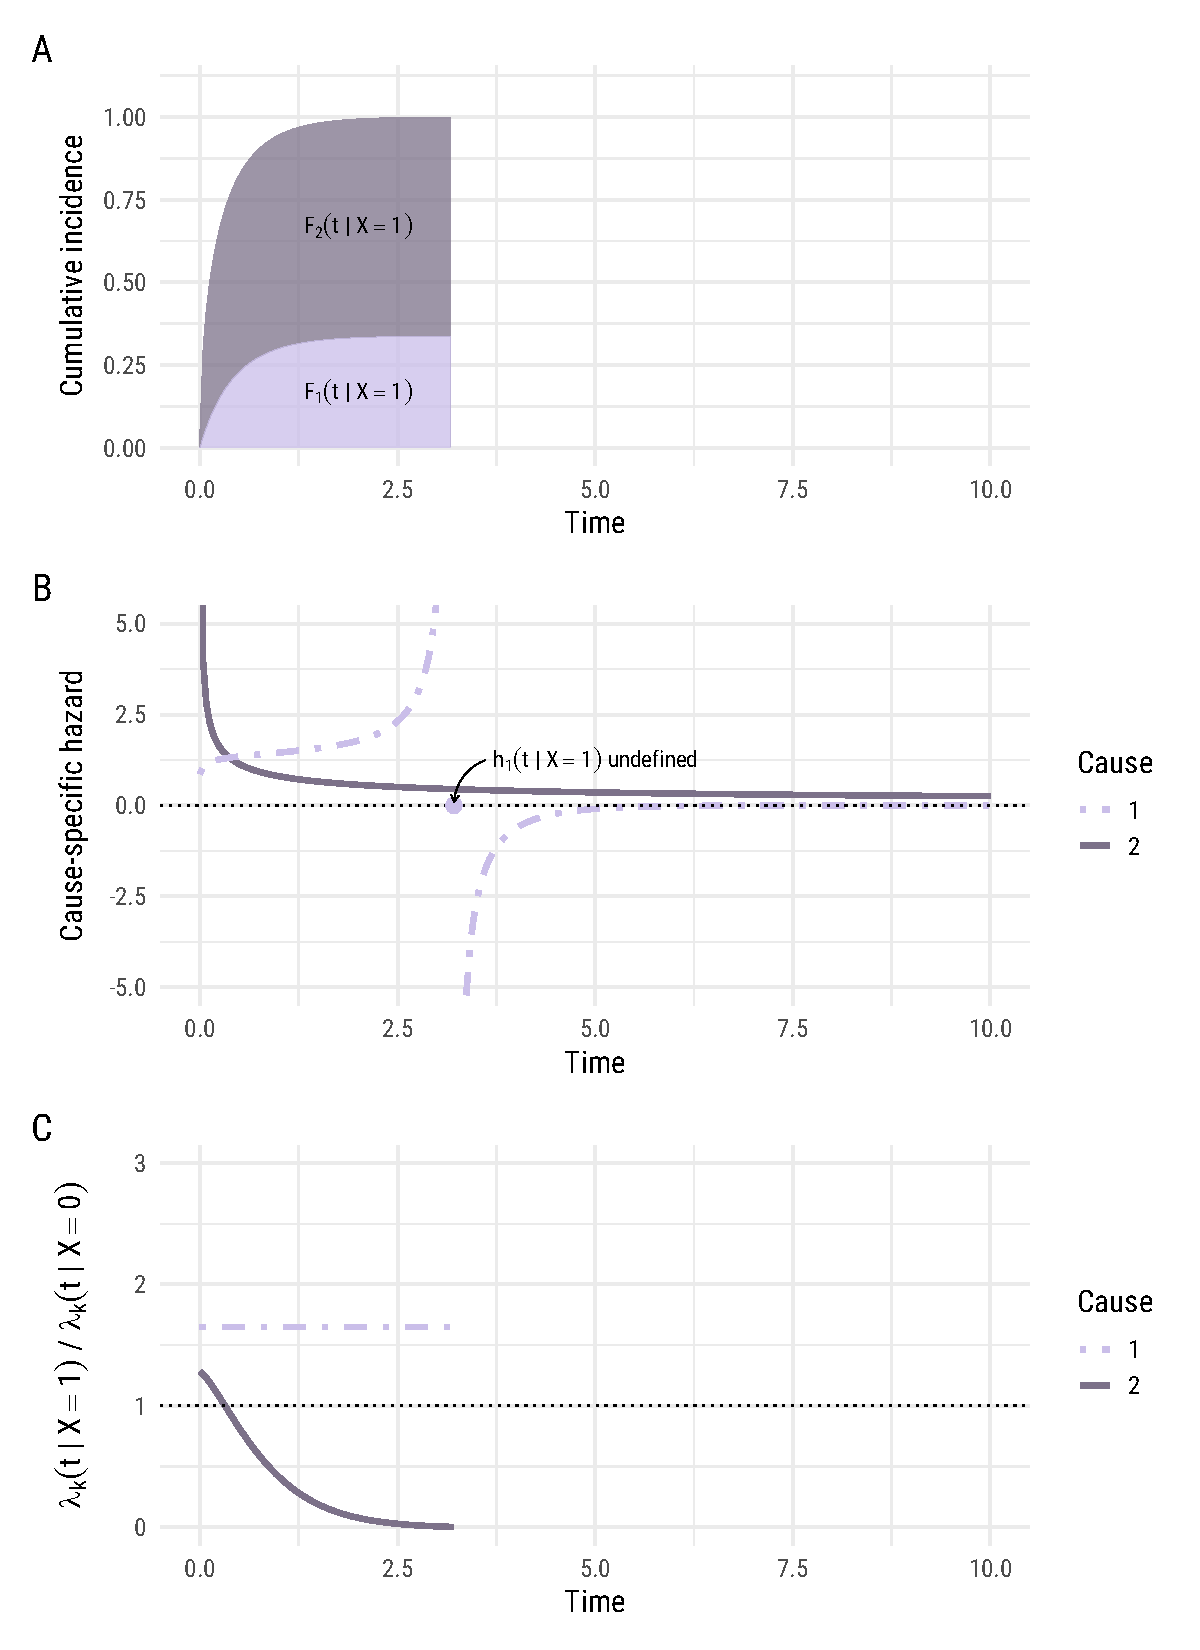
\includegraphics[width=0.8\textwidth,height=\textheight]{chapters/../figures/fine-gray-DGM_reduc.pdf}

}

\caption{\label{fig-reduc}True stacked cumulative incidence functions
(panel A) and cause-specific hazards (panel B) conditional on \(X = 1\),
and the subdistribution hazard ratios (panel C) for both causes, under
DGM described in Section~\ref{sec-reduct-int}. This DGM assumes a
Fine--Gray model for cause 1 with Gompertz baseline subdistribution
hazard, and cause-specific Cox model for cause 2 with a Weibull baseline
hazard.}

\end{figure}

\hypertarget{specifying-lambda_1t-given-x-and-h_1t-given-x}{%
\subsubsection{\texorpdfstring{Specifying \(\lambda_1(t \given X)\) and
\(h_1(t \given X)\)}{Specifying \textbackslash lambda\_1(t \textbackslash given X) and h\_1(t \textbackslash given X)}}\label{specifying-lambda_1t-given-x-and-h_1t-given-x}}

If we instead choose to specify both the subdistribution and
cause-specific hazards for event 1, the cause-specific hazard for cause
2 can be derived by re-arranging Equation~\ref{eq-reduc} as
\begin{equation}\protect\hypertarget{eq-sdh1-csh1}{}{
h_2(t \given X) = \lambda_1(t \given X) - h_1(t \given X) - \frac{\diff}{\diff t} \log \Biggl\{ \frac{\lambda_1(t \given X)}{h_1(t \given X)}\Biggr\}.
}\label{eq-sdh1-csh1}\end{equation} While a Gompertz baseline hazard
could again be specified for \(\lambda_1(t \given X)\), it is important
to specify \(h_1(t \given X)\) such that
\(h_1(t \given X) = \lambda_1(t \given X)\) at \(t = 0\). From a
simulator's point of view, it means paying attention to the fact that
due to the form of the reduction factor (a time-dependent weight),
proportionality generally cannot hold for both \(\lambda_1(t \given X)\)
and \(h_1(t \given X)\) simultaneously. If the Fine--Gray model holds
for \(\lambda_1(t \given X)\), the cause-specific hazard ratio
\(h_1(t \given X=1) / h_1(t \given X=0)\) should usually be
time-dependent.

An exception to the above is found in the work of Saadati \emph{et al.}
(\protect\hyperlink{ref-saadatiPredictionAccuracyVariable2018}{2018}).
There, a DGM is presented where \(h_2(t \given X)\) is chosen such that
proportionality holds on both the subdistribution and cause-specific
hazard scale for cause 1. The chosen \(h_2(t \given X)\) is based on
setting the reduction factor to 1 for all covariate patterns and
timepoints, which also implies that the covariate effects on the
subdistribution and cause-specific hazard for event 1 need to be equal
to each other.

Similarly to Equation Equation~\ref{eq-sdh1-csh2}, the implied
\(h_2(t \given X)\) when specifying \(\lambda_1(t \given X)\) and
\(h_1(t \given X)\) may also become negative. To understand an instance
of where this can occur, note that we can write the all-cause cumulative
hazard as a function of \(\lambda_1(t \given X)\) and
\(h_1(t \given X)\) using Equation \eqref{eq:reduc}, as
\begin{equation*}
    -\log\{S(t \given X)\} = \frac{\lambda_1(t \given X) \exp\{-\Lambda_1(t \given X)\}}{h_1(t \given X)}.
\end{equation*} As an example, we can use the same Gompertz
parametrisation for \(\lambda_1(t \given X)\) as in the previous
sub-section, namely \(\{\kappa_1, \nu_1, \beta_1\} = \{-2, 0.5, 0.5\}\).
Suppose now we also decide to use a Gompertz baseline hazard for
\(h_1(t \given X)\), using the same parametrisation (i.e.~base rate also
equal to \(\nu_1\) and \(\beta_1 = \gamma_1\), ensuring
\(\lambda_1(t \given X) = h_1(t \given X)\) at \(t = 0\)), but instead
setting the shape parameter to 2 (exponentially increasing). By solving
\(-\log\{S(t \given X)\} - H_1(t \given X) = 0\), one can find the
timepoint at which \(H_1(t \given X)\) starts to exceed the all-cause
cumulative hazard. Prior to this timepoint, \(H_2(t \given X)\) will be
forced to decrease in order to maintain
\(-\log\{S(t \given X)\} = H_1(t \given X) + H_2(t \given X)\), implying
negative \(h_2(t \given X)\). Note also that this is not the fault of
the Gompertz distribution: it is perfectly possible to simulate
competing risks data with baseline cause-specific Gompertz hazards.

From a simulator's point of view, a DGM based on directly specified
\(\lambda_1(t \given X)\) and \(h_1(t \given X)\) is rather tedious to
implement given (a) the restriction that
\(\lambda_1(t \given X) = h_1(t \given X)\) at \(t = 0\) for all \(X\),
(b) the (generally) time-dependent nature of the cause-specific hazard
ratio for event 1. Even when \(\beta_1 = \gamma_1\) (same covariate
effects on cause-specific and subdistribution hazard of cause 1), which
is unlikely to be the case in practice unless there are relatively few
cause 2 failures, specifying an adequate \(h_1(t \given X)\) is not very
flexible. As part of work on simulating proportional subdistribution
hazard data with time-varying effects, Haller and Ulm
(\protect\hyperlink{ref-hallerFlexibleSimulationCompeting2014}{2014})\}
provide an example of simulating from a DGM based on specifying both
\(h_1(t \given X)\) and \(\lambda_1(t \given X)\). There,
\(h_1(t \given X)\) is chosen to be time constant, with rate equal to
\(\lambda_1(t \given X)\) at \(t = 0\).

\hypertarget{specifying-lambda_1t-given-x-and-a-model-for-the-all-cause-hazard}{%
\subsubsection{\texorpdfstring{Specifying \(\lambda_1(t \given X)\) and
a model for the all-cause
hazard}{Specifying \textbackslash lambda\_1(t \textbackslash given X) and a model for the all-cause hazard}}\label{specifying-lambda_1t-given-x-and-a-model-for-the-all-cause-hazard}}

The reduction factor could also form the basis for a DGM if a model is
specified for the all-cause hazard
\(\sum_{k = 1}^{K} H_k(t \given X) = -\log\{S(t \given X)\}\), together
with the Fine--Gray model for \(\lambda_1(t \given X)\). One can derive
the implied \(h_1(t \given X)\) from Equation \eqref{eq:reduc}, and
subtract it from the all-cause hazard to obtain \(h_2(t \given X)\).
Proportional hazards on the all-cause scale however typically implies
that the cause-specific hazards will be non-proportional. Note that this
DGM requires that \(-\log\{S(t \given X)\} > \Lambda_1(t \given X)\) at
all timepoints and for all \(X\). That is, that the all-cause cumulative
hazard is always greater than the cumulative subdistribution hazard of
event 1, otherwise the implied cause-specific hazard for cause 2 is
forced to be negative. When simulating from this DGM, this could for
example occur if the specified covariate effects differ substantially
between the subdistribution hazard model for cause 1 and the all-cause
model (e.g.~pushing \(\Lambda_1(t \given X)\) above
\(-\log\{S(t \given X)\}\) for \(X = 1\)). Nevertheless, as long as
precautions are taken when specifying \(-\log\{S(t \given X)\}\), this
DGM again represents a valid way to specify \(f(T, D \given X)\) such
that proportional subdistribution hazards hold for cause 1. To the best
of our knowledge, this mechanism has not been used in articles
simulating proportional subdistribution hazards data.

\hypertarget{squeezing}{%
\subsection{Squeezing}\label{squeezing}}

Instead of specifying the various hazard functions, we can also work
with the cumulative incidence functions directly. Recall that the
Fine--Gray model for cause 1 can be expressed as \begin{align*}
    1 - F_1(t \given X) = \{1 - F_{10}(t)\}^{\exp(\beta_1 X)}.
\end{align*} The idea is now to specify \(F_{10}(t)\) directly. Since
\(F_k(\infty)=P(D=k)<1\), we have to first pick some proper cumulative
distribution \(\tilde{F}_{10}(t)\) (e.g.~exponential or Weibull
cumulative distribution function, CDF) with
\(\lim_{t \to \infty}\tilde{F}_{10}(t) = 1\) and scale it down by a
factor \(0< p < 1\) (since \(p = 0\) or \(p = 1\) would imply no
competing risks). This leaves \begin{equation*}
    1 - F_1(t \given X) = \big[1-p\{ \tilde{F}_{10}(t) \}\big]^{\exp(\beta_1 X)}.
\end{equation*} Note that \(\lim_{t \to \infty}F_{10}(t) = p\), and
\(p_1(x) = P(D = 1 \given X) = 1 - (1-p)^{\exp(\beta_1 X)}\). The
probability of experiencing cause 2 therefore needs to be ``squeezed''
into the remaining probability space
\(p_2(x) = P(D = 2 \given X) = 1 - P(D = 1 \given X) = (1-p)^{\exp(\beta_1 X)}\).
Since \(p_2(x)\) is determined by \(p_1(x)\), it is guaranteed that
\(p_1(x) + p_2(x) = 1\). The second cumulative incidence function takes
the form \begin{equation*}
    P(T \leq t, D=2 \given X) = P(T \leq t \given D=2, X)P(D = 2 \given X),
\end{equation*} where \(P(T \leq t \given D=2, X)\) can be chosen to be
any standard CDF, which is then scaled down by \(P(D = 2 \given X)\).
When simulating using this DGM, it is convenient to first generate the
competing event indicator, and thereafter draw event times conditional
on this indicator e.g.~for event 1, drawing from
\(P(T \leq t \given D=1, X)\). For more details, see section 5.3.6 of
Beyersmann \emph{et al.}
(\protect\hyperlink{ref-beyersmannCompetingRisksMultistate2012}{2012}).
This DGM is arguably the most commonly used approach to simulate
proportional subdistribution hazard data, as it ensures the TFP remains
below or equal to 1. Multiple simulation studies, along with the
original article proposing the Fine--Gray model, have simulated data in
this way Austin \emph{et al.}
(\protect\hyperlink{ref-austinFineGraySubdistributionHazard2021}{2021}).

To illustrate this mechanism, we use Weibull-type distribution functions
and set \begin{align*}
    \tilde{F}_{10}(t) &= 1 - \exp(-b_1t^{a_1}), \\
    P(T \leq t \given D=2, X) &= 1 - \exp\{-b_2t^{a_2}\exp(\beta^*_2 X)\},
\end{align*} with \(\{a_1, b_1, \beta_1, p\} = \{1.25, 1, 0.5, 0.2\}\)
and \(\{a_2, b_2,\beta^*_2\} = \{1.5, 1, 0.5\}\). \(\beta^*_2\) is
denoted as such since it is not a subdistribution log hazard ratio, but
instead denotes the effect of \(X\) on \(P(T \leq t \given D=2, X)\).
Figure~\ref{fig-squeeze} shows the baseline hazards and hazard ratios
(\(X = 1\) relative to \(X = 0\)) over time for the cause-specific and
subdistribution hazards of both events. For this DGM, these functions
are arguably more interesting to show, since they are only implicitly
specified e.g.~\(h_1(t \given X)\) is obtained by dividing
\(\diff F_1(t \given X)/\diff t\) by
\(1 - F_1(t \given X) - F_2(t \given X)\). Note that in panels B and D
(and also in panel C in Figure~\ref{fig-reduc}), no logarithmic
transformation was applied to the y-axis (as would normally be the case
for hazard ratio plots) due to the cause-specific and subdistribution
hazard ratios for cause 2 going to zero as \(t \to \infty\).

This DGM provides a clear picture on why one may choose to avoid
Fine--Gray models for more than one cause. As other authors have
similarly noted
(\protect\hyperlink{ref-beyersmannCompetingRisksMultistate2012}{Beyersmann
\emph{et al.}, 2012}), a Fine--Gray model being specified for cause 1
effectively constrains the remaining probability space available to
cause 2 to a maximum of \(1 - P(D = 1 \given X)\). Equivalently, this is
a constraint on
\(\Lambda_2(t \given X) = -\log\{1 - F_2(t \given X)\}\), the cumulative
subdistribution hazard for cause 2 conditional on \(X\). In the case of
a binary \(X\), this translates to the coefficient of a Fine--Gray model
for the competing cause needing to be \textit{determined} by the
Fine--Gray model for cause 1. Explictly, we can express the cumulative
subdistribution hazard ratio for cause 2 as \(t \to \infty\) for this
DGM as \begin{align*}
    \lim_{t \to \infty} \frac{\Lambda_{2}(t \given X = 1)}{\Lambda_{2}(t \given X = 0)} &= \frac{-\log\{1 - P(D = 2 \given X = 1)\}}{-\log\{1 - P(D = 2 \given X = 0)\}} ,\\
    &= \frac{\log \{P(D = 1 \given X = 1)\}}{\log \{P(D = 1 \given X = 0)\}}, \\
    &= \frac{\log \{1 - (1-p)^{\exp(\beta_1)}\}}{\log(p)},
\end{align*} by using
\(P(D = 2 \given X) = 1 - \exp\{- \lim_{t \to \infty} \Lambda_2(t \given X)\}\)
and \(P(D = 2 \given X) = 1 - P(D = 1 \given X)\). Therefore, the
cumulative subdistribution hazard ratio for cause 2 as \(t \to \infty\)
should be completely determined by \(\beta_1\) and \(p\). Since running
a Fine--Gray model for the second cause does not account for this
restriction, it is typically misspecified, leading to issues such as the
TFP exceeding 1. As shown in Figure~\ref{fig-squeeze}, the extent of
this misspecification can be alarming: the true subdistribution hazard
ratio for the competing cause is severely time-dependent, for which the
time-averaged subdistribution hazard ratio (see Grambauer \emph{et al.}
(\protect\hyperlink{ref-grambauerProportionalSubdistributionHazards2010}{2010}))
obtained from a Fine--Gray model is perhaps a suboptimal summary.

\begin{figure}

{\centering 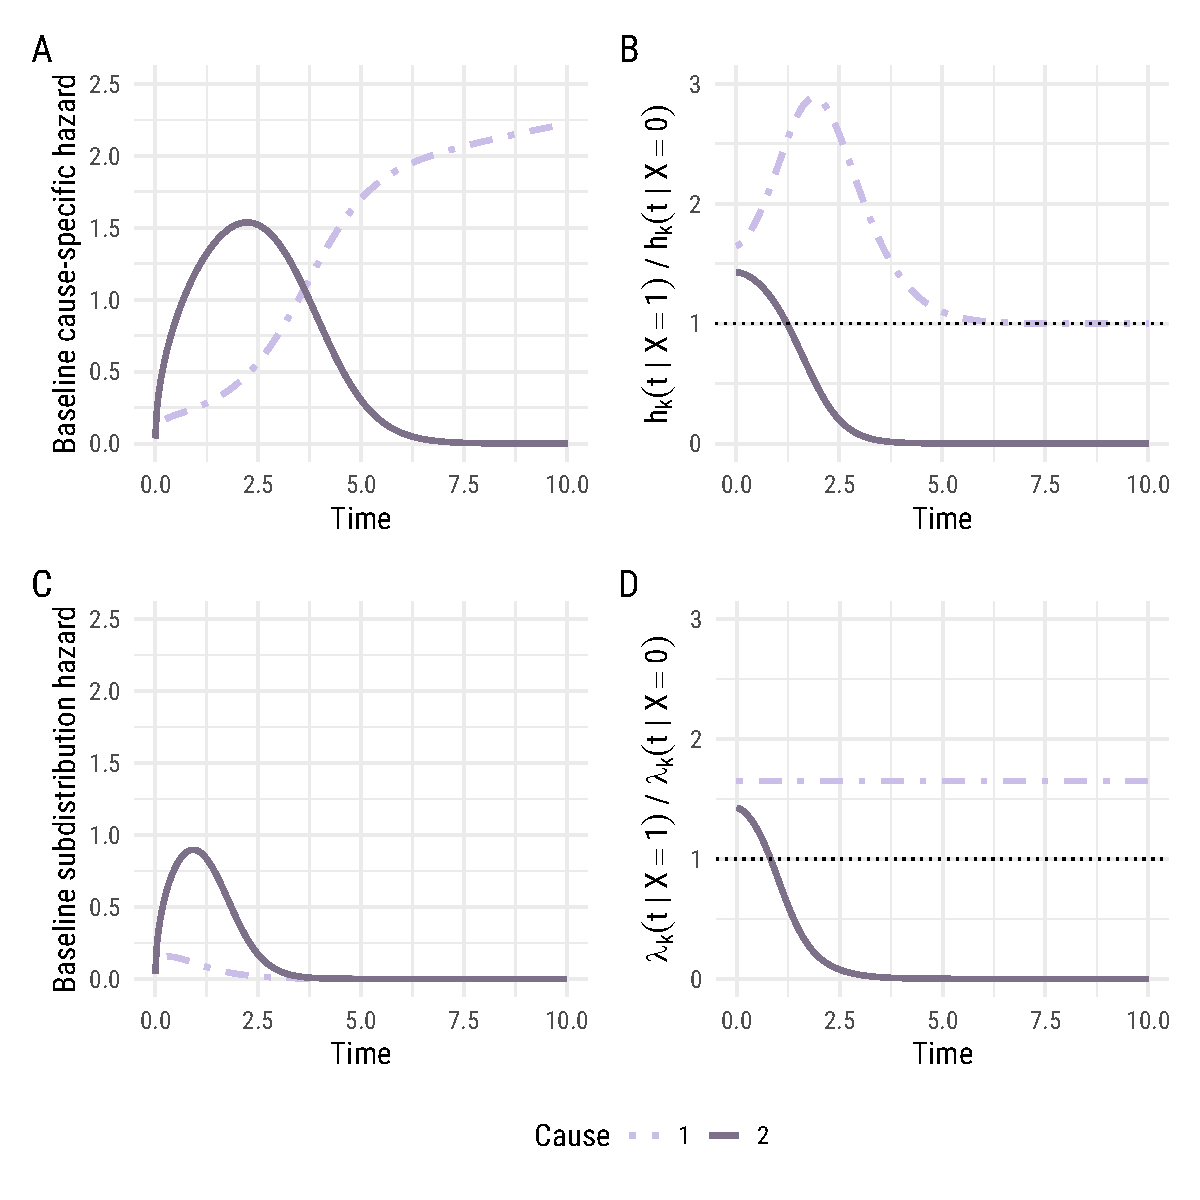
\includegraphics[width=0.9\textwidth,height=\textheight]{chapters/../figures/fine-gray-DGM_squeeze.pdf}

}

\caption{\label{fig-squeeze}Baseline hazards (panels A and C) and hazard
ratios \(X = 1\) relative to \(X = 0\) (panels B and D) over time for
the cause-specific and subdistribution hazards of both events, based on
`squeezing' DGM.}

\end{figure}

\hypertarget{two-finegray-models}{%
\subsection{Two Fine--Gray models}\label{two-finegray-models}}

The previous sub-section may suggest that it is impossible for
proportional subdistribution hazards to hold for more than one competing
event. In fact, if we choose to also directly specify the cumulative
incidence for cause 2 in the same style as in the ``squeezing''
mechanism (instead of having it determined by cause 1), we can achieve
proportional subdistribution hazards for both events. Suppose we have
\begin{align*}
    F_1(t \given X) &= 1 - \big[1 - p_{10}\{\tilde{F}_{10}(t)\} \big]^{\exp(\beta_1X)}, \\
    F_2(t \given X) &= 1 - \big[1 - p_{20}\{\tilde{F}_{20}(t)\} \big]^{\exp(\beta_2X)}.
\end{align*} If we let
\(P(D = k \given X) = 1 - (1 - p_{k0})^{\exp(\beta_{k}X)} = p_k(x)\),
then we can write that as \(t \to \infty\),
\(\text{TFP}(x) = p_1(x) + p_2(x)\). To determine the event indicator
when simulating, we would draw \(u \sim \mathcal{U}(0,1)\), and set
\begin{equation*}
    D = 
    \begin{cases}
        1, & \text{if}\ u \leq p_1(x), \\
        2, & \text{if}\ p_1(x) < u \leq p_2(x). 
    \end{cases}
\end{equation*} The event times can then be drawn as in the preceding
subsection, by inverting \(P(T \leq t \given D=k, X)\). Those with
\(u > p_1(x) + p_2(x)\) are technically considered ``cured'\,', that is,
never at risk of any of the competing events. To illustrate this DGM, we
set \begin{align*}
    \tilde{F}_{10}(t) &= 1 - \exp(-b_1t^{a_1}), \\
    \tilde{F}_{20}(t) &= 1 - \exp(-b_2t^{a_2}),
\end{align*} with
\(\{a_1, b_1, \beta_1, p_{10}\} = \{0.75, 1, 0.5, 0.25\}\) and
\(\{a_2, b_2,\beta_{2}, p_{20}\} = \{0.75, 1, 0.5, 0.5\}\).
Figure~\ref{fig-twofgs} shows the baseline cumulative incidence
functions, and those conditional on \(X = 1\). The chosen baseline
cumulative incidence functions and subdistribution hazard ratios result
in the TFP exceeding 1 from \(t \approx 3\) when \(X = 1\). While this
mechanism can be flexible when baseline hazard rates are small and
covariate effects are modest, it by design cannot guarantee a TFP
\(\leq 1\) for any timepoint. Indeed, if \(X\) is not binary, and
instead continuous and unbounded, the TFP is guaranteed to exceed 1
(though for small \(t\), \(X\) will need to be very extreme for this to
occur)
(\protect\hyperlink{ref-austinFineGraySubdistributionHazard2021}{Austin
\emph{et al.}, 2021}).

Two other useful implementations of (variants of) this DGM are found in
the simulations of Mao and Lin
(\protect\hyperlink{ref-maoEfficientEstimationSemiparametric2017}{2017}),
and Mozumder \emph{et al.}
(\protect\hyperlink{ref-mozumderDirectLikelihoodInference2018}{2018}) -
both investigating the performance of different approaches
(semiparametric and flexible parametric, respectively) for direct
modelling of the cumulative incidence functions. Mao and Lin directly
specify Gompertz cumulative subdistribution hazards
\(\Lambda_k(t \given X)\) for both events, and thereafter invert
\(P(T \leq t \given D=k, X)\) analogously using
\(P(T \leq t, D=k \given X) = 1 - \exp\{-\Lambda_k(t \given X)\}\) and
its limit as \(t \to \infty\). Mozumbder et al.~specify mixture Weibull
baseline subdistribution hazards for both events, and then derive the
implied cause-specific hazards using the reduction factor, and use these
for simulating.

An important point is that both of the above approaches specify a
maximum follow-up time in their simulations. Indeed, as pointed out by
Latouche \emph{et al.}
(\protect\hyperlink{ref-latoucheCompetingRisksAnalysis2013}{2013}), ``it
is possible that such models may hold over restricted time ranges, which
has practical implications for studies with limited longitudinal
follow-up'', with ``such models'' referring to multiple proportional
subdistribution hazard models. Note also that specifying a maximum
follow-up time \(\tau\) means that the
\(1 - F_1(\tau \given X) - F_2(\tau \given X)\) proportion of
individuals that did not experience the event by \(\tau\) are simply
considered as censored at \(\tau\).

\begin{figure}

{\centering 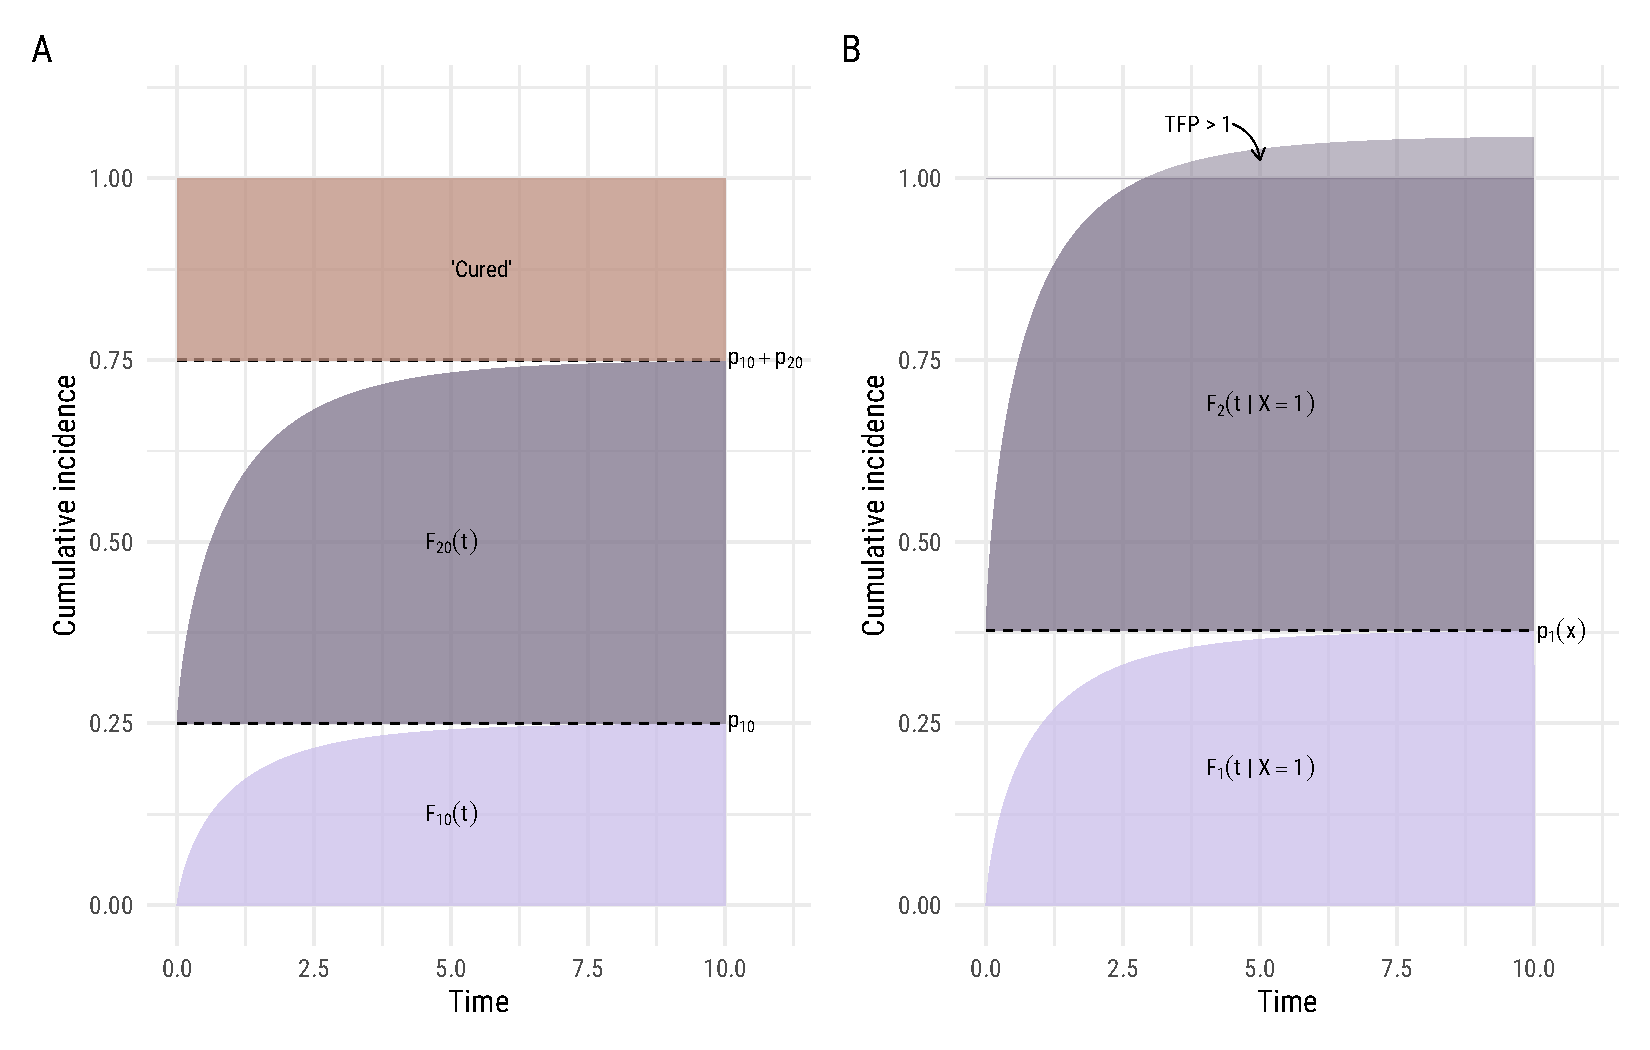
\includegraphics[width=0.95\textwidth,height=\textheight]{chapters/../figures/fine-gray-DGM_twofgs.pdf}

}

\caption{\label{fig-twofgs}Stacked cumulative incidence functions
conditional on \(X = 0\) (baseline, panel A) and those conditional on
\(X = 1\) (panel B), for a DGM in which proportional subdistribution
hazards can hold for both causes.}

\end{figure}

\hypertarget{discussion}{%
\section{Discussion}\label{discussion}}

In this work, we have outlined various ways of specifying a joint
density \(f(T, D \given X)\) in which a Fine--Gray model for cause 1 is
correctly specified. The goal was to outline the possible assumptions
that can be made regarding the (cumulative incidence of) cause 2, given
that a Fine--Gray model is correctly specified for cause 1. From a
simulator's perspective, all DGMs are fundamentally aiming to do the
same thing, which is to fill up the probability space leftover from the
assumed Fine--Gray model for cause 1 i.e.~\(1 - F_1(t \given X)\). The
``squeezing'' DGM does this in the most explicit way, by making sure
cause 2 fills up all of the remaining space, in turn ensuring that the
TFP remains below or equal to 1 for all \(X\) and at all timepoints.
This makes it the approach with the fewest restrictions when simulating
data for which proportional subdistribution hazards holds for one cause
only. Using the reduction factor in contrast can be quite inflexible,
possibly producing negative cause-specific hazard values without great
care in choices of parameter values and distributions. Note also that
the described DGMs can be readily adapted in order to simulate under
link functions other than the complementary log-log, discussed for
example by Gerds \emph{et al.}
(\protect\hyperlink{ref-gerdsAbsoluteRiskRegression2012a}{2012}). More
generally, there is no DGM for which proportional subdistribution
hazards holds simultaneously for both causes, unless one assumes finite
follow-up and a bounded covariate space.

Suppose that we have a dataset where proportional subdistribution
hazards perfectly hold for both causes up to some maximum follow-up
time, e.g.~a simulated dataset, for which we know the DGM. Here, fitting
a Fine--Gray model for each cause in turn (i.e.~using the exact models
the data were generated from) can still lead to the TFP exceeding 1.
This can occur more generally in finite samples, since the Fine--Gray
models for each cause are estimated separately. As a result, alternative
approaches have been developed (based on the complete data likelihood)
to facilitate simultaneous modelling of all cumulative incidence
functions, while incorporating this TFP constraint
(\protect\hyperlink{ref-maoEfficientEstimationSemiparametric2017}{Mao
and Lin, 2017};
\protect\hyperlink{ref-shiConstrainedParametricModel2013}{Shi \emph{et
al.}, 2013}) The parametric approach suggested by Shi \emph{et al.}
(\protect\hyperlink{ref-shiConstrainedParametricModel2013}{2013})\}
actually does so by explicitly incorporating the ``squeezing'\,' of the
second cause (i.e.~that covariates effects on cause 2 depend on the
asymptote of the cumulative incidence function for cause 1) into the
likelihood. Note also that modelling the cause-specific hazards and
combining these to obtain predicted cumulative incidence functions
ensures that the TFP remains below 1 for any timepoint and covariate
combination
(\protect\hyperlink{ref-austinFineGraySubdistributionHazard2021}{Austin
\emph{et al.}, 2021}). The cause-specific approach also extends
naturally (i.e.~without TFP issues or tedious algebra) to settings with
more than two competing events.

In applied settings, proportionality assumptions for either event on any
of cause-specific and subdistribution hazard scales, such as those made
in the outlined DGMs, will never hold exactly. Using alloSCT data, Gerds
\emph{et al.}
(\protect\hyperlink{ref-gerdsAbsoluteRiskRegression2012a}{2012})
compared the performance of cause-specific hazard and Fine--Gray models
(as well as other transformation models) for predicting competing events
relapse and non-relapse mortality. Both predictive accuracy (based on
cross-validated Brier score) and individual predictions were similar for
both approaches. Wolbers \emph{et al.}
(\protect\hyperlink{ref-wolbersPrognosticModelsCompeting2009}{2009})\}
reported that the cause-specific and Fine--Gray approaches showed
comparable calibration when predicting coronary heart disease, though
they did not consider calibration of the competing event. Kantidakis
\emph{et al.}
(\protect\hyperlink{ref-kantidakisStatisticalModelsMachine2023}{2023})
also reported similar predictive performance of the cause-specific and
Fine--Gray approaches when applied on a dataset of patients with
extremity soft-tissue sarcoma. This was as part of a broader comparison
with machine learning techniques, with the goal of predicting competing
events disease progression and death.

One explanation for this comparable performance is that both models make
use of their non-parametric baseline hazard to compensate, to some
extent, for misspecified (i.e.~non-proportional) covariate effects -
allowing them to still predict the cumulative incidence functions fairly
accurately (noted in Shi \emph{et al.}
(\protect\hyperlink{ref-shiConstrainedParametricModel2013}{2013}) for
Fine--Gray models). Differences in performance may also be modest in
settings with a shorter follow-up period or when there is heavy
censoring: the time-dependent weight relating the cause-specific and
subdistribution hazards (the reduction factor) is less influential
earlier in time. Nevertheless, there are situations in which one would
expect (multiple) Fine--Gray models to underperform with respect to
cause-specific hazard approaches. First, when the estimated TFP exceeds
1 in a non-negligible proportion of patients, as in the example by
Austin \emph{et al.}
(\protect\hyperlink{ref-austinFineGraySubdistributionHazard2021}{2021}),
the predictions for one or more of the competing events must by
definition be partly miscalibrated (due to risk overestimation). Second,
when the true cumulative incidence curves for an event (e.g.~relapse
probabilities for two conditioning regimens) cross each other, the
predicted curves by the Fine--Gray model will not be allowed to cross.
Poythress \emph{et al.}
(\protect\hyperlink{ref-poythressPlanningAnalyzingClinical2020a}{2020})
therefore suggest to compare predicted curves to their non-parametric
counterparts as a possible diagnostic, and note that cause-specific
hazards models are much more suited to capturing more complex cumulative
incidence function shapes. For example, the cause-specific hazards could
be modelled using flexible parametric approaches, which naturally
accommodate time-varying effects
(\protect\hyperlink{ref-hinchliffeFlexibleParametricModelling2013}{Hinchliffe
and Lambert, 2013};
\protect\hyperlink{ref-kipourouEstimationAdjustedCausespecific2019}{Kipourou
\emph{et al.}, 2019}).

In conclusion, the described DGMs outline the variety of ways in which
proportional subdistribution hazards could hold for at least one of two
event types. In terms of cumulative incidence prediction for both
causes, we argue that cause-specific hazard models should be preferred
over multiple Fine--Gray models, as they (a) by design ensure that the
TFP does not exceed 1, (b) are able to capture complex shapes for the
cumulative incidence functions (although in the Fine--Gray context, one
could technically include time by covariate interactions), and (c)
additionally provide inference on the cause-specific hazards, which are
the ``natural building blocks for competing risks modeling'\,'
(\protect\hyperlink{ref-saadatiPredictionAccuracyVariable2018}{Saadati
\emph{et al.}, 2018}). The \texttt{\{riskRegression\}} R package in
particular provides useful functions for developing and validating
prediction models based on cause-specific hazards
(\protect\hyperlink{ref-RJ-2017-062}{Ozenne \emph{et al.}, 2017}). While
using a Fine--Gray model for one cause only may still be defendable
(e.g.~for prediction purposes, when other causes are truly a nuisance),
it does go against the holistic approach to competing risks analyses
described in the introduction, where all causes should ideally be
studied together. Cause-specific hazard models, which are often
misunderstood to be less suitable for prediction compared to Fine--Gray
models (see e.g. D'Amico \emph{et al.}
(\protect\hyperlink{ref-damicoClinicalStatesCirrhosis2018}{2018})),
should perhaps also be the preferred approach also in settings where
predicting a single cause is of interest. When the main goal is
simultaneous inference on the cumulative incidence functions, the
proposed semiparametric approach by Mao and Lin
(\protect\hyperlink{ref-maoEfficientEstimationSemiparametric2017}{2017})
is a promising alternative to multiple Fine--Gray models, as it (a)
provides more efficient inference, (b) allows the use of different link
functions (e.g.~accommodates non-proportional hazards, and allows odds
ratio interpretation of parameters) for different events, (c) does not
need to model the censoring distribution. For inference at specific
timepoints, one may also consider to specify models using pseudovalues
as the outcome variable
(\protect\hyperlink{ref-kleinRegressionModelingCompeting2005a}{Klein and
Andersen, 2005}).

\bookmarksetup{startatroot}

\hypertarget{joint-models-quantify-associations-between-immune-cell-kinetics-and-allo-immunological-events-after-allogeneic-stem-cell-transplantation-and-subsequent-donor-lymphocyte-infusion}{%
\chapter{Joint models quantify associations between immune cell kinetics
and allo-immunological events after allogeneic stem cell transplantation
and subsequent donor lymphocyte
infusion}\label{joint-models-quantify-associations-between-immune-cell-kinetics-and-allo-immunological-events-after-allogeneic-stem-cell-transplantation-and-subsequent-donor-lymphocyte-infusion}}

Alloreactive donor-derived T-cells play a pivotal role in alloimmune
responses after allogeneic hematopoietic stem cell transplantation
(alloSCT); both in the relapse-preventing Graft-versus-Leukemia (GvL)
effect and the potentially lethal complication Graft-versus-Host-Disease
(GvHD). The balance between GvL and GvHD can be shifted by removing
T-cells via T-cell depletion (TCD) to reduce the risk of GvHD, and by
introducing additional donor T-cells (donor lymphocyte infusions
{[}DLI{]}) to boost the GvL effect. However, the association between
T-cell kinetics and the occurrence of allo-immunological events has not
been clearly demonstrated yet. Therefore, we investigated the complex
associations between the T-cell kinetics and alloimmune responses in a
cohort of 166 acute leukemia patients receiving alemtuzumab-based TCD
alloSCT. Of these patients, 62 with an anticipated high risk of relapse
were scheduled to receive a prophylactic DLI at 3 months after
transplant. In this setting, we applied joint modelling which allowed us
to better capture the complex interplay between DLI, T-cell kinetics,
GvHD and relapse than traditional statistical methods. We demonstrate
that DLI can induce detectable T-cell expansion, leading to an increase
in total, CD4+ and CD8+ T-cell counts starting at 3 months after
alloSCT. CD4+ T-cells showed the strongest association with the
development of alloimmune responses: higher CD4 counts increased the
risk of GvHD (hazard ratio 2.44, 95\% confidence interval 1.45-4.12) and
decreased the risk of relapse (hazard ratio 0.65, 95\% confidence
interval 0.45-0.92). Similar models showed that natural killer cells
recovered rapidly after alloSCT and were associated with a lower risk of
relapse (HR 0.62, 95\%-CI 0.41-0.93). The results of this study advocate
the use of joint models to further study immune cell kinetics in
different settings.

\hfill\break

\hypertarget{introduction-4}{%
\section{Introduction}\label{introduction-4}}

The curative potential of allogeneic stem cell transplantation (alloSCT)
in the treatment of hematological malignancies depends on the
introduction of donor-derived alloreactive T-cells
(\protect\hyperlink{ref-horowitzGraftversusleukemiaReactionsBone1990}{Horowitz
\emph{et al.}, 1990}). These T-cells recognize non-self antigens on
patient-derived cells and can, once activated, expand and eliminate
those cells. Targeting antigens on lymphohematopoietic cells including
the malignant cells leads to the desired Graft-versus-Leukemia (GvL)
effect and prevents relapse. However, when other tissues of the patient
are targeted, Graft-versus-Host-Disease (GvHD) may develop
(\protect\hyperlink{ref-falkenburgGraftTumorEffects2017}{Falkenburg and
Jedema, 2017}). Natural killer (NK) cells may discriminate between
healthy and non-healthy (e.g., virus-infected or malignant) cells by
acting on signals from inhibitory and activating receptors that bind to
the target cell. In the setting of alloSCT, early NK cell recovery can
protect against relapse and viral infections
(\protect\hyperlink{ref-dunbarRelationshipCirculatingNatural2008}{Dunbar
\emph{et al.}, 2008};
\protect\hyperlink{ref-minculescuEarlyNaturalKiller2016}{Minculescu
\emph{et al.}, 2016}). However, NK cells do not appear to be important
effector cells in GvHD
(\protect\hyperlink{ref-simonettaNaturalKillerCells2017}{Simonetta
\emph{et al.}, 2017}).

To reduce the risk of severe GvHD, donor T-cell depletion (TCD) can be
applied, although this will decrease the GvL effect
(\protect\hyperlink{ref-buscaInvivoExvivoCell2017}{Busca and Aversa,
2017}). In order to restore the GvL effect to prevent relapse, TCD
alloSCT can be combined with the administration of donor lymphocyte
infusions (DLIs) after transplant
(\protect\hyperlink{ref-eeftingMyeloablativeCelldepletedAlloSCT2014}{Eefting
\emph{et al.}, 2014};
\protect\hyperlink{ref-eeftingMultistateAnalysisIllustrates2016}{Eefting
\emph{et al.}, 2016};
\protect\hyperlink{ref-falkenburgGraftTumorEffects2017}{Falkenburg and
Jedema, 2017}). DLI as part of a pre-emptive strategy is administered to
patients with detectable minimal residual disease (MRD) or with residual
patient hematopoiesis: mixed chimerism (MC). DLI as part of a
prophylactic strategy is given to all patients in whom no GvHD has
developed as sign of alloreactivity. The alloreactive potential of DLI
decreases over time after alloSCT: both the efficacy (GvL effect) and
toxicity (GvHD) are highest early after alloSCT
(\protect\hyperlink{ref-krishnamurthyOutcomeDonorLymphocyte2013}{Krishnamurthy
\emph{et al.}, 2013};
\protect\hyperlink{ref-yunFindingSweetSpot2013}{Yun and Waller, 2013}).
Therefore, administration preferably starts a few months after alloSCT
to allow for sufficient GvL without severe GvHD
(\protect\hyperlink{ref-frederik2019delayed}{Frederik Falkenburg
\emph{et al.}, 2019}).

Since T-cells are pivotal for alloimmune responses, several groups have
investigated T-cell kinetics after alloSCT and their impact on the
development of GvHD or relapse. However, as shown in the recent review
by Yanir \emph{et al.}
(\protect\hyperlink{ref-yanirImmuneReconstitutionAllogeneic2022}{2022}),
the reported results are inconsistent, and their interpretation is
complicated by several factors. First, T-cells can be patient- or
donor-derived, while only donor-derived T-cells are responsible for GvHD
and GvL. Second, the T-cell changes following alloSCT are the combined
result of de novo T-cell generation from infused hematopoietic stem
cells starting at least 6 months after alloSCT, homeostatic
proliferation of T-cells present in the patient or graft, T-cell
expansion during infections and expansion of alloreactive T-cells
responsible for GvL and GvHD. Especially cytomegalovirus (CMV)
reactivations are common during the first 3 months after alloSCT and
strongly affect the kinetics of both T-cells and NK cells after alloSCT
(\protect\hyperlink{ref-boschImmuneReconstitutionAntithymocyte2012a}{Bosch
\emph{et al.}, 2012};
\protect\hyperlink{ref-hassanCMVReactivationInitiates2022}{Hassan
\emph{et al.}, 2022};
\protect\hyperlink{ref-sternImmunoprofilingRevealsCell2022}{Stern
\emph{et al.}, 2022}). This may distort the association between the
kinetics of the main T-cell subsets and specific alloimmune responses,
i.e., the presence of GvHD and the absence of relapse as a result of the
GvL effect. Third, factors that could influence both the T-cell kinetics
and the risks of GvHD and relapse, such as the conditioning regimen,
donor type and the use and method of TCD, should be properly accounted
for. Finally, ignoring clinical events or interventions during follow-up
can also be problematic: over time, the patients that have not yet
experienced an event like relapse, death or the development of GvHD,
become less representative of the population at the beginning of
follow-up. As death by definition prevents further T-cell measurements
and the possibility of experiencing subsequent GvHD and relapse, bias is
created by considering the patients who died as having non-informatively
dropped out (i.e.~that their measurements could have been measured if
kept under follow-up). Likewise, DLI and the use of posttransplant
prophylactic immunosuppression are known to affect the risks of relapse
and GvHD, but may also affect the T-cell kinetics
{[}lewalleDonorLymphocyteInfusions2003;Schmaelter \emph{et al.}
(\protect\hyperlink{ref-schmaelterAlterationsPeripheralBlood2021}{2021});Bellucci
\emph{et al.}
(\protect\hyperlink{ref-bellucciImmunologicEffectsProphylactic2002}{2002});Guillaume
\emph{et al.}
(\protect\hyperlink{ref-guillaumeEscalatedLymphodepletionFollowed2012}{2012});Nikiforow
\emph{et al.}
(\protect\hyperlink{ref-nikiforowPhaseStudyCD252016}{2016});Schultze-Florey
\emph{et al.}
(\protect\hyperlink{ref-schultze-floreyClonalExpansionCD82021}{2021});Toor
\emph{et al.}
(\protect\hyperlink{ref-toorDynamicalSystemModeling2015}{2015});Gooptu
\emph{et al.}
(\protect\hyperlink{ref-gooptuEffectSirolimusImmune2019}{2019}){]}. To
fully understand the complex interplay between all these factors,
sophisticated statistical methods are required that properly model the
T-cell kinetics themselves, along with their association with GvHD or
relapse. Joint modelling captures the T-cell trajectories and the
clinical events simultaneously, accounting for informative dropout, as
well as the measurement error and heterogeneity in individual
trajectories
(\protect\hyperlink{ref-rizopoulosJointModelsLongitudinal2012}{Rizopoulos,
2012}).

In this study, we performed joint modelling to investigate the complex
associations between the immune cell kinetics and alloreactivity in a
cohort of 166 patients receiving an alloSCT for acute leukemia or
myelodysplastic syndrome (MDS). All patients received an
alemtuzumab-based TCD alloSCT after nonmyeloablative conditioning
without any posttransplant prophylactic immunosuppression. Patients with
an anticipated high risk of relapse were scheduled to receive an early
low-dose DLI prophylactically at 3 months after alloSCT, while
prophylactic DLI administration for the other patients started at 6
months. In this unique setting we investigated the impact of the early
low-dose DLI on the T-cell and NK cell kinetics during the first 6
months after transplant and the association between these kinetics and
the development of clinical events.

\hypertarget{methods-2}{%
\section{Methods}\label{methods-2}}

\hypertarget{study-population}{%
\subsection{Study population}\label{study-population}}

This retrospective study included all adult patients with acute myeloid
leukemia, acute lymphoblastic leukemia or MDS in complete morphologic
remission after intensive induction therapy who received their first
alloSCT from a 9 or 10 out of 10 HLA matched donor using
nonmyeloablative conditioning and alemtuzumab-based TCD
(\protect\hyperlink{ref-vondemborneReducedintensityConditioningAllogeneic2009a}{von
dem Borne \emph{et al.}, 2009}) between March 2008 and December 2019 at
Leiden University Medical Center (LUMC, Leiden, The Netherlands). Two
patients who were transplanted while receiving systemic
immunosuppression for a non-transplant indication (polymyalgia
rheumatica and cryptogenic organizing pneumonia) were excluded because
of the potential impact of the ongoing systemic immunosuppression on the
immune cell recovery after alloSCT. All patients signed informed consent
for data collection and analysis. Data were analyzed as of July 2021.

\hypertarget{transplantation-and-dli-strategy}{%
\subsection{Transplantation and DLI
strategy}\label{transplantation-and-dli-strategy}}

As conditioning regimen patients received either fludarabine (6 days 50
mg/m2 orally or 30 mg/m2 intravenously) and busulfan (2 days 4x0.8 mg/kg
intravenously), or the FLAMSA regimen: fludarabine (5 days 30 mg/m2
intravenously), cytarabine (4 days 2000 mg/m2 intravenously), amsacrine
(4 days 100 mg/m2 intravenously) and busulfan (4 days 4x0.8 mg/kg
intravenously). In both regimens, TCD was performed by adding 20 mg
alemtuzumab (Sanofi Genzyme, Naarden, The Netherlands) to the graft
before infusion and by administering 15 mg alemtuzumab intravenously on
days -4 and -3. Patients with an unrelated donor (UD) received
rabbit-derived anti-thymocyte globulin (ATG; Sanofi Genzyme)
additionally on day -2 (until April 2010 2mg/kg and thereafter 1mg/kg).
None of the patients received posttransplant GvHD prophylaxis.

The dose of unmodified pre-emptive and prophylactic DLIs was based on
donor type and timing after alloSCT. Standard DLIs given at 6 months
after alloSCT contained 3x106 or 1.5x106 T-cells/kg for patients with a
related donor (RD) or an UD, respectively. Early low-dose DLIs given at
3 months after alloSCT contained 0.3x106 or 0.15x106 T-cells/kg for
patients with a RD or an UD, respectively. Since May 2010, all patients
without any relapse and without GvHD requiring systemic
immunosuppressive treatment at 6 months after alloSCT prophylactically
(i.e., irrespective of chimerism or posttransplant MRD status) were
planned to receive the standard DLI. Patients who were considered to
have a high risk of relapse based on the disease characteristics or MRD
status at time of alloSCT or who received the FLAMSA regimen were also
scheduled to receive the early low-dose DLI prophylactically at 3 months
after alloSCT. All patients, including those transplanted before May
2010, could receive pre-emptive DLIs in case of MC or MRD positivity,
starting from 3 months after alloSCT. Additionally, as part of several
clinical trials, patients could receive modified T-cell products
prophylactically or virus-specific T-cell infusions to treat severe
viral infections.

\hypertarget{monitoring-of-cmv-and-absolute-numbers-of-circulating-immune-cells}{%
\subsection{Monitoring of CMV and absolute numbers of circulating immune
cells}\label{monitoring-of-cmv-and-absolute-numbers-of-circulating-immune-cells}}

CMV serostatus was assessed in all patients and donors before alloSCT.
After transplant CMV was monitored routinely by PCR on peripheral blood
samples in all patients. Absolute numbers of circulating total (CD3+),
CD4+CD8- and CD4-CD8+ T-cells, B cells and NK cells were measured
routinely at predefined timepoints on anticoagulated fresh venous blood
by flow cytometry with bead calibration (Trucount tubes, BD
Biosciences). Samples were measured either on a FACSCalibur using
anti-CD3-APC, anti-CD4-FITC, anti-CD8-PE, and anti-CD45-PerCP or with
anti-CD3-FITC, anti-CD16-PE, anti-CD19-APC, anti-CD45-PerCP, and
anti-CD56-PE, or on a FACSCanto using anti-CD3-APC, anti-CD4-PB,
anti-CD8-FITC, anti-CD16-PE, anti-CD19-PE Cy7, anti-CD45-PerCP, and
anti-CD56-PE (all from BD). The lower detection limit was 0.5x106
cells/L.

\hypertarget{definitions-of-events}{%
\subsection{Definitions of events}\label{definitions-of-events}}

Relapse was defined as the recurrence of at least 5\% blasts on
cytomorphologic bone marrow examination or at least 1\% blasts in
peripheral blood (if possible, confirmed by BM biopsy). We defined
clinically significant GvHD as the start of therapeutic systemic
immunosuppression for GvHD
(\protect\hyperlink{ref-kosterCompetitiveRepopulationAlloImmunologic2023}{Koster
\emph{et al.}, 2023}). We defined `other failure' as the occurrence of
an adverse event with a potential impact on the immune cell kinetics:
death, graft failure, start of systemic immunosuppression for a non-GvHD
indication, and virus-specific T-cell infusion for a severe viral
infection (whichever occurred first). Graft failure was defined as the
occurrence of \textgreater95\% patient BM chimerism in all lineages
tested or refractory granulopenia (granulocyte count \textless0.5x109/l)
in the absence of relapse or ongoing myelotoxic medication.

For this study we analyzed the T-cell and NK cell kinetics and events
during the first 6 months after alloSCT, during which the early
immunological recovery and most CMV reactivations take place.
Furthermore, during this period the impact of the early low-dose DLI can
be assessed, as the standard DLI is given to all eligible patients
around 6 months after alloSCT. As part of the analyses assessing the net
impact of the early low-dose DLI on the T-cell and NK cell kinetics and
clinical events, patients receiving a standard DLI or modified T-cell
product as part of a clinical trial were censored at 7 days after this
infusion. We considered this to be non-informative censoring, since
these interventions were prophylactic and not driven by the clinical
course of the patient. For the T-cell kinetics we considered the
circulating cell counts of the total (CD3+) T-cell population and the
two major T-cell subpopulations: the CD4+CD8- and the CD4-CD8+ T-cells.

\hypertarget{statistical-analyses}{%
\subsection{Statistical analyses}\label{statistical-analyses}}

Probabilities of overall survival (OS) and relapse-free survival (RFS)
after alloSCT with associated 95\% confidence intervals (95\%-CI) were
calculated by the Kaplan-Meier method. The cumulative incidences of
clinically significant GvHD and relapse from time of alloSCT were
estimated by means of the Aalen-Johansen method, treating other failure
(as described in the previous section) as a third competing risk.

To study the complex interplay between the immune cell kinetics, DLI and
clinically relevant endpoints (GvHD and relapse), two joint models were
developed; model I starting at time of alloSCT and model II at time of
the early low-dose DLI.

Shared-parameter joint models consist of two components: a longitudinal
submodel, and a time-to-event submodel
(\protect\hyperlink{ref-rizopoulosJointModelsLongitudinal2012}{Rizopoulos,
2012}). The former often takes the form of a mixed-effects regression
model, and the latter is generally assumed to follow a proportional
hazards structure, similar to a Cox model (for one or possibly multiple
endpoints such as GvHD or relapse). The mixed-effects model allows to
model cell count trajectories over time, while appropriately accounting
for both the heterogeneity in subject-specific trajectories (using
random effects) and measurement error. These two submodels are linked
together via an association structure. Practically speaking, this allows
the hazard of a particular event to depend on characteristics of an
individual's specific trajectory, such as the `true' underlying (i.e.~in
absence of measurement error) value over time. In turn, this enables the
estimation of an association between a longitudinal marker (e.g.~CD3
counts) and the risk of a clinical event (e.g.~GvHD). In the presence of
an association, the estimated trajectories themselves will be corrected
for bias related to the measurements being terminated by the occurrence
of endpoints (generally known as `informative dropout').

Below follows a concise description of the joint models developed for
the present application. Detailed explanation of the statistical models
and the underlying rationale can be found in the Statistical Supplement.
For all models, absolute cell counts were analyzed on the log scale
after setting measurements under the detection limit to 0.5. This only
occurred at earliest timepoints where because of the lymphodepletion by
the conditioning regimen and TCD, the counts are expected to be around
zero.

\hypertarget{model-i-starting-from-allosct}{%
\subsubsection{Model I (starting from
alloSCT)}\label{model-i-starting-from-allosct}}

To investigate the effect of early low-dose DLI on the kinetics of the
T-cell and NK cell counts after TCD alloSCT, we performed an
intention-to-treat (ITT) analysis with a baseline group distinguishing
between those scheduled for early low-dose DLI because of a high
anticipated risk of relapse (henceforth `high risk' group) and those who
were not (`non-high risk' group). We chose this approach instead of a
per-protocol analysis since we could not properly define a control group
of patients who did not receive early DLI but could have been candidates
as we did not know for each patient who was not scheduled for early DLI
whether he/she would have been able to receive it.

Figure 1A shows a schematic overview of joint model I. The model was run
separately for each T-cell subset, respectively using CD3, CD4 or CD8
counts, and the total NK counts. All patients started at time of alloSCT
and were followed-up until 6 months after alloSCT or until the
occurrence of an earlier endpoint (GvHD, relapse or other failure),
whichever occurred first. The longitudinal submodel was a linear
mixed-effects model, which used restricted cubic splines to flexibly
model the log counts over time. The baseline covariates included in this
submodel were disease risk (non-high risk or high risk), donor type (RD
or UD with ATG-containing conditioning regimen) and patient/donor CMV
status (both seronegative {[}CMV -/-{]} or not). The patient/donor CMV
status was included as simple fixed effect, and both disease risk and
donor type were included as part of a three-way interaction with time.
This was in order to both properly accommodate the expected slower
lymphocyte recovery in patients treated with ATG, and to evaluate a
difference in trajectories between the disease risk groups. The
time-to-event submodel comprised three cause-specific proportional
hazards models, with GvHD, relapse and other failure as competing
events. As predictors, they each contained the time-dependent current
value (i.e.~the underlying `true' value at a given timepoint, as
estimated by the longitudinal submodel) of the log immune cell count, as
well as the baseline factors donor type and disease risk. The latter was
omitted as a covariate from the model for `other failure' due to the
limited number of events.

To investigate whether the current slope (i.e.~rate of increase or
decrease of counts at a given moment) of the T-cell counts was
associated with the development of GvHD, we also extended the models by
adding the current slope of the log counts in addition to the current
value to the time-to-event submodel (so-called `time-dependent slopes'
parametrization).

\hypertarget{model-ii-starting-from-early-low-dose-dli}{%
\subsubsection{Model II (starting from early low-dose
DLI)}\label{model-ii-starting-from-early-low-dose-dli}}

To further investigate the T-cell kinetics after the early low-dose DLI,
we constructed a joint model including only the patients who actually
received the early low-dose DLI without any prior event of interest
(Figure 1B). Since NK cells recover rapidly after alloSCT
(\protect\hyperlink{ref-elfekyImmuneReconstitutionFollowing2019a}{Elfeky
\emph{et al.}, 2019}) (expected before the administration of early
low-dose DLI in this study), they were not considered for model II. The
time-scale was taken from DLI instead of from alloSCT, and follow-up was
restricted to 3 months after this DLI, until administration of a second
DLI, or until the occurrence of a terminating event, whichever occurred
first. The disease risk factor was omitted since all included patients
belonged to the high risk group. Since only 7 patients had a non-GvHD
event within 3 months after the early low-dose DLI (Supplementary Figure
1), relapse and other failure were combined into one composite endpoint
to compete with GvHD and the donor type factor was omitted for this
composite endpoint.

\hypertarget{software-3}{%
\subsection{Software}\label{software-3}}

All analyses were performed in R version 4.2.1 using the packages JM
(\protect\hyperlink{ref-rizopoulosJMPackageJoint2010}{Rizopoulos, 2010})
(version 1.5-2), survival
(\protect\hyperlink{ref-survival-package}{Therneau, 2023}) (version
3.4.0) and nlme
(\protect\hyperlink{ref-pinheiroNlmeLinearNonlinear2023}{Pinheiro
\emph{et al.}, 2023}) (3.1-157). Full code needed to reproduce the
results of the present work is available at
https://github.com/survival-lumc/ImmuneReconstJM, and structured using
the targets
(\protect\hyperlink{ref-landauTargetsPackageDynamic2021}{Landau, 2021})
(version 0.14.0) package.

\hypertarget{results-3}{%
\section{Results}\label{results-3}}

\hypertarget{population}{%
\subsection{Population}\label{population}}

166 patients were included in this study. Baseline characteristics are
presented in Table 1. All surviving patients had at least 12 months
follow-up since alloSCT. OS and RFS at 6 months after alloSCT were 77\%
(95\%-CI 71-83) and 70\% (95\%-CI 64-77), respectively. A total of 62
patients were considered to have a high risk of relapse and were
scheduled for an early low-dose DLI, of whom 42 actually received it
after a median interval of 3.1 months (range: 2.7-4.4) without any prior
event of interest (Supplementary Figure 1). Twenty patients did not
receive an early low-dose DLI: 10 because of early relapse, 9 because of
early other failures (death {[}n=1{]}, graft failure {[}n=2{]}, start of
systemic immunosuppression for a non-GvHD indication {[}n=4{]}, or
administration of a virus-specific T-cell infusion {[}n=2{]}), and 1
patient did not receive the early low-dose DLI because of mild skin GvHD
requiring topical treatment. All 19 events occurred within 4 months
after alloSCT. The patient with mild skin GvHD remained event-free for
at least 51 months after alloSCT. None of the 104 non-high risk patients
received an early low-dose DLI. At 6 months after alloSCT, the
cumulative incidence of clinically significant GvHD was 26\% (95\%-CI
15-37) and 5\% (95\%-CI 0-9) for the high risk patients scheduled for
early low-dose DLI and the non-high risk patients, respectively
(Supplementary Figure 2). All clinically significant GvHD in the high
risk patients occurred after administration of the early low-dose DLI
(but before standard DLI) of which 88\% occurred in patients receiving
DLI from an UD after an ATG-containing conditioning regimen.

\begingroup\fontsize{9}{11}\selectfont

\hypertarget{tbl-table-one}{}
\begin{longtable}[t]{>{\raggedright\arraybackslash}p{15em}>{\raggedright\arraybackslash}p{8em}>{\raggedright\arraybackslash}p{8em}>{\raggedright\arraybackslash}p{8em}}
\caption{\label{tbl-table-one}\emph{Baseline characteristics}. Intention for early low-dose DLI is
based on the anticipated high risk of relapse after alloSCT. DLI, donor
lymphocyte infusion; alloSCT, allogeneic stem cell transplantation; AML,
acute myeloid leukemia; ALL, acute lymphoblastic leukemia; MDS,
myelodysplastic syndrome; Flu, fludarabine; Bu, busulfan; Ara-C,
cytarabine; Amsa, amsacrine; RD, related donor; UD, unrelated donor;
GCSF, granulocyte-colony stimulation factor; PBSC, peripheral blood stem
cells; BM, bone marrow. *One patient had not received a second
consolidation course before transplant and received 2 days
cyclophosphamide 750 mg/m2 intravenously additionally to the
conditioning regimen. }\tabularnewline

\toprule
 & Total cohort (n = 166) & Intention for early low-dose DLI (n = 62) & No intention for early low-dose DLI (n = 104)\\
\midrule
\addlinespace[0.3em]
\multicolumn{4}{l}{\textbf{Age at alloSCT (years)}}\\
\hspace{1em}median (range) & 63 (28-78) & 64 (31-78) & 63 (28-73)\\
\addlinespace[0.3em]
\multicolumn{4}{l}{\textbf{Disease}}\\
\hspace{1em}AML & 133 (80\%) & 46 (74\%) & 87 (84\%)\\
\hspace{1em}ALL & 17 (10\%) & 10 (16\%) & 7 (7\%)\\
\hspace{1em}MDS & 16 (10\%) & 6 (10\%) & 10 (10\%)\\
\addlinespace[0.3em]
\multicolumn{4}{l}{\textbf{Nonmyeloablative conditioning}}\\
\hspace{1em}Flu/Bu & 150 (90\%) & 46 (74\%) & 104 (100\%)\\
\hspace{1em}Flu/Bu/Ara-C/Amsa (FLAMSA) & 16 (10\%) & 16 (26\%) & 0\\
\addlinespace[0.3em]
\multicolumn{4}{l}{\textbf{Donor}}\\
\hspace{1em}RD, 10/10 HLA matched & 57 (34\%) & 20 (32\%) & 37 (36\%)\\
\hspace{1em}UD, 10/10 HLA matched & 101 (61\%) & 39 (63\%) & 62 (60\%)\\
\hspace{1em}UD, 9/10 HLA matched & 8 (5\%) & 3 (5\%) & 5 (5\%)\\
\addlinespace[0.3em]
\multicolumn{4}{l}{\textbf{Graft source}}\\
\hspace{1em}G-CSF mobilized PBSC & 165 (99\%) & 62 (100\%) & 103 (99\%)\\
\hspace{1em}BM & 1 (1\%) & 0 & 1 (1\%)\\
\addlinespace[0.3em]
\multicolumn{4}{l}{\textbf{CMV serostatus patient/donor}}\\
\hspace{1em}Patient +/Donor + & 79 (48\%) & 32 (52\%) & 47 (45\%)\\
\hspace{1em}Patient +/Donor - & 25 (15\%) & 8 (13\%) & 17 (16\%)\\
\hspace{1em}Patient -/Donor + & 11 (7\%) & 4 (6\%) & 7 (7\%)\\
\hspace{1em}Patient -/Donor - & 51 (31\%) & 18 (29\%) & 33 (32\%)\\
\addlinespace[0.3em]
\multicolumn{4}{l}{\textbf{Main reason for intention for early low-dose DLI}}\\
\hspace{1em}FLAMSA regimen & - & 16 (26\%) & -\\
\hspace{1em}MRD+ at time of alloSCT & - & 14 (23\%) & -\\
\hspace{1em}AML/MDS: EVI1 overexpression & - & 9 (15\%) & -\\
\hspace{1em}AML: monosomal karyotype & - & 8 (13\%) & -\\
\hspace{1em}AML: ASXL mutation, only one & - & 4 (6\%) & -\\
\hspace{1em}remission induction course, or &  &  & \\
\hspace{1em}persisting underlying disease &  &  & \\
\hspace{1em}ALL: t(9;22) & - & 4 (6\%) & -\\
\hspace{1em}ALL: hypodiploidy, no CR1, or & - & 4 (6\%) & -\\
\hspace{1em}t(4;11) &  &  & \\
\hspace{1em}Therapy-related AML & - & 2 (3\%) & -\\
\hspace{1em}AML: progression before alloSCT & - & 1 (2\%) & -\\
\bottomrule
\end{longtable}
\endgroup{}

\hypertarget{t-cell-trajectories-after-allosct-and-dli}{%
\subsection{T-cell trajectories after alloSCT and
DLI}\label{t-cell-trajectories-after-allosct-and-dli}}

\hypertarget{dli-related-increase-of-t-cell-counts-after-3-months-after-allosct-observed-in-patients-with-an-unrelated-donor}{%
\subsubsection{DLI-related increase of T-cell counts after 3 months
after alloSCT observed in patients with an unrelated
donor}\label{dli-related-increase-of-t-cell-counts-after-3-months-after-allosct-observed-in-patients-with-an-unrelated-donor}}

To investigate whether administration of the early low-dose DLI
increased the numbers of circulating T-cells during the first 6 months
after alloSCT, we performed an ITT analysis using model I (see Methods)
to compare the 62 high risk patients who were scheduled for early
low-dose DLI with the 104 non-high risk patients who were not. All
patients had at least 2 T-cell measurements with a median of 6
measurements per patient (interquartile range: 5-8). Although patients
showed very different T-cell kinetics over time (Supplementary Figure
3), the model was flexible enough to capture the different shapes of
patient-specific trajectories (Figure 2). Patients who were CMV
seropositive or who had a CMV seropositive donor had significantly
higher CD3 and CD8 counts during the first 6 months after TCD alloSCT
compared to CMV seronegative patients with a CMV seronegative donor,
corresponding to a significant increase on the log scale of 0.49
(95\%-CI 0.31-0.67) and 0.45 (95\%-CI 0.08-0.80) for CD3+ and CD8+
T-cells, respectively. For instance, the model-based CD3 count at 6
months for a non-high risk patient with a RD was 425x106/l if CMV -/-
compared to 694x106/l for any other CMV serostatus combination. The
model-based CD8 count at this time was 222x106/l compared to 347x106/l,
respectively, suggesting expansion of CMV-specific T-cells. A same trend
was observed for the CD4 counts (increase of 0.11 on the log scale,
95\%-CI 0-0.23). As shown in Figure 3, patients with an UD had lower
T-cell counts during the first 3 months after TCD alloSCT than patients
with a RD, illustrating the enduring effect of the additional ATG that
was given to all patients with an UD. We observed no significant
difference in the cell count trajectories between the disease risk
groups for patients with a RD. In contrast, in patients with an UD the
CD4 trajectories started to diverge at 3 months after alloSCT, resulting
in higher cell counts in the high risk patients intended to receive an
early low-dose DLI at 3 months. The CD3 and CD8 counts showed similar
trends. Taken together, these data show that a strategy of early
low-dose DLI can lead to T-cell expansion.

\hypertarget{cd3-cd4-and-cd8-counts-increase-after-early-low-dose-dli}{%
\subsubsection{CD3, CD4 and CD8 counts increase after early low-dose
DLI}\label{cd3-cd4-and-cd8-counts-increase-after-early-low-dose-dli}}

To investigate whether the T-cell counts increased after the early
low-dose DLI as the ITT-analysis suggested, we used model II including
only the 42 patients who actually received this DLI without any prior
event and modelled the kinetics during the first 3 months after DLI. One
of the 42 patients did not have any T-cell measurement during this
period and was excluded. Baseline characteristics of the 41 included
patients are described in Supplementary Table 1. These patients had at
least one T-cell measurement during the 3-month period after early
low-dose DLI with a median of 4 measurements (interquartile range: 2-5).
Again, a flexible model was constructed to capture the different shapes
of the T-cell kinetics of the included patients (Supplementary Figure 4
and Supplementary Figure 5). The model-based trajectories of the total,
CD4+ and CD8+ T-cell counts (Figure 4) showed increasing T-cell counts
after DLI, with similar effects of the patient/donor CMV serostatus and
donor type on the T-cell counts as in the earlier models.

\hypertarget{associations-between-t-cell-kinetics-and-alloimmune-responses-after-allosct-and-dli}{%
\subsection{Associations between T-cell kinetics and alloimmune
responses after alloSCT and
DLI}\label{associations-between-t-cell-kinetics-and-alloimmune-responses-after-allosct-and-dli}}

\hypertarget{higher-cd3-and-cd4-counts-are-associated-with-a-higher-risk-of-gvhd}{%
\subsubsection{Higher CD3 and CD4 counts are associated with a higher
risk of
GvHD}\label{higher-cd3-and-cd4-counts-are-associated-with-a-higher-risk-of-gvhd}}

To study the association between the T-cell kinetics and the development
of GvHD or relapse after TCD alloSCT and DLI, we added disease risk and
donor type as time-fixed covariates alongside the time-dependent T-cell
counts in the cause-specific submodels (with GvHD, relapse and other
failure as competing events) of model I. As shown in Figure 5, donor
type showed no significant association with the risk of GvHD, although
in the CD4 model a trend for higher risk in patients with an UD despite
the ATG in the conditioning regimen was observed (hazard ratio {[}HR{]}
2.7, 95\%-CI 1.0-7.4). High risk patients, who were scheduled for early
low-dose DLI, had a considerably higher risk of GvHD compared to
non-high risk patients with HRs ranging between 6.3 (CD8 model, 95\%-CI
2.1-18.8) and 7.3 (CD4 model, 95\%-CI 2.4-22.2), indicating an
alloimmune effect of the early low-dose DLI in this setting. The current
values of the log CD4 and CD3 counts significantly increased the risk of
GvHD (HR 2.4 (95\%-CI 1.4-4.1) and HR 1.5 (95\%-CI 1.0-2.3) for CD4+
T-cells and CD3+ T-cells, respectively), while CD8+ T-cells showed a
similar trend (HR 1.3, 95\%-CI 0.9-1.8). These HRs represent the
relative increase in GvHD risk for an increase of one in the log counts,
assuming same disease risk and donor type. These results indicate that
the absolute total numbers of circulating CD4+ and CD3+ T-cells after
alloSCT and DLI are informative for the development of GvHD.

We hypothesized that not only the current value but also the slope of
the T-cell counts would be associated with the development of an
alloimmune response. To investigate this, we extended the time-to-event
submodel of model I by additionally including the current slope of the
T-cell counts as a covariate for all endpoints. However, we observed no
association between the slope of any of the T-cell subsets and the
development of GvHD (p-values 0.59-0.87). We therefore retained the
simpler version of model I with only the current value.

\hypertarget{protective-effect-of-cd4-t-cells-against-relapse-and-other-failure}{%
\subsubsection{Protective effect of CD4+ T-cells against relapse and
other
failure}\label{protective-effect-of-cd4-t-cells-against-relapse-and-other-failure}}

To investigate whether higher T-cell counts were associated with a lower
risk of relapse, we examined the risk factors for relapse in the
time-to-event submodel of model I. Despite the ATG, patients with an UD
had a significantly lower risk of relapse than patients with a RD (HRs
ranging between 0.2 (95\%-CI 0.1-0.5) and 0.3 (95\%-CI 0.1-0.8), Figure
5). A trend was observed for higher relapse risk in the high risk
patients (HR 2.1 in all models, 95\%-CI for CD4+ T-cells: 0.9-5.0,
respectively), suggesting that the addition of early low-dose DLI to the
strategy did not completely compensate for the higher relapse risk.
While CD3+ and CD8+ T-cells showed no significant association with
relapse, higher CD4 counts decreased the risk of relapse significantly
(HR 0.6, 95\%-CI 0.5-0.9).

Of the 36 patients who experienced other failures, 6 died, 8 developed
graft failure, 18 required systemic immunosuppression for a non-GvHD
indication (of whom 9 received rituximab for EBV) and 4 received a
virus-specific T-cell infusion for a severe viral infection. Only in the
CD8 model a trend was observed for a higher risk of other failure in
patients with an UD receiving an ATG-containing conditioning regimen (HR
2.6, 95\%-CI 1.0-6.9). Higher CD4+ T-cell counts significantly lowered
the hazard of the composite endpoint other failure (HR 0.7, 95\%-CI
0.6-1.0).

\hypertarget{t-cell-counts-after-early-low-dose-dli-retain-their-association-with-the-development-of-gvhd}{%
\subsubsection{T-cell counts after early low-dose DLI retain their
association with the development of
GvHD}\label{t-cell-counts-after-early-low-dose-dli-retain-their-association-with-the-development-of-gvhd}}

To investigate whether the T-cell kinetics were also associated with the
development of alloimmune responses in the postDLI setting, we used the
time-to-event submodel of model II starting from early low-dose DLI with
GvHD and non-GvHD events as competing events. We observed no significant
association between the current values and the very heterogenous
composite endpoint of relapse and other failure (Figure 6). However,
patients with an UD had a considerably higher risk of GvHD with HRs
ranging between 7.0 (CD8+ T-cells, 95\%-CI 1.5-32.1) and 22.5 (CD4+
T-cells, 95\%-CI 3.7-138.9) compared to patients with a RD. For all
T-cell subsets, higher current values increased the risk of GvHD with
HRs ranging between 1.6 (CD8+ T-cells, 95\%-CI 1.0-2.6) and 6.7 (CD4+
T-cells, 95\%-CI 2.1-21.5). These data show that in the subset of
patients receiving early low-dose DLI, total CD3+, CD4+ and CD8+ T-cell
counts after DLI are associated with the development of GvHD.

\hypertarget{nk-cell-kinetics-and-associations-with-alloimmune-responses-after-allosct}{%
\subsection{NK cell kinetics and associations with alloimmune responses
after
alloSCT}\label{nk-cell-kinetics-and-associations-with-alloimmune-responses-after-allosct}}

To investigate the NK cell kinetics and their association with GvHD and
relapse, we returned to model I starting at alloSCT. As shown in
Supplemental Figure 6, the NK cell counts recovered rapidly, reaching
the normal levels of 40-390x106 NK cells/l for almost all patients
within 2 months, before the time of administration of the early low-dose
DLI. As shown in Figure 7, CMV seropositive patients or patients with a
CMV seropositive donor had significantly higher NK counts than CMV -/-
patients, as was seen for the T-cell subsets. In contrast to T-cell
kinetics, patients with an UD and ATG did not have a slower recovery of
NK counts compared to patients with a RD and no ATG. Furthermore, there
was no association between the risk group and NK counts, indicating that
there was no impact of DLI on the NK cell kinetics. Higher current NK
counts were associated with a higher risk of GvHD (HR 1.95 per unit log
count increase, 95\%-CI 1.10-3.47) and a lower risk of relapse (HR 0.62,
95\%-CI 0.41-0.93) but had no significant association with the risk of
other failure. We hypothesized that the observed association between the
NK count and GvHD may not be due to a direct effect of the NK cells, but
instead reflected the high correlation between the NK and CD4 count
trajectories, the latter being expected to be the main driver of GvHD.
We therefore ran a cause-specific Cox model for GvHD, which included
disease risk and donor type as time-fixed covariates, and both CD4 and
NK counts as time-dependent covariates. In this model, CD4 counts were
significantly associated with the development of GvHD (HR 2.08, 95\%-CI
1.16-3.74) while the HR for the NK cell counts was 1.07 (p-value 0.83),
supporting that the CD4+ T-cells were the important drivers for the
development of GvHD.

\hypertarget{discussion-1}{%
\section{Discussion}\label{discussion-1}}

In this study we investigated the interplay between immune cell kinetics
and alloimmune responses after both TCD alloSCT and subsequent DLI using
joint modelling. In the ITT analysis we observed significantly more GvHD
in the high risk patients intended to receive an early low-dose DLI and
an increase in T-cell counts starting at 3 months after alloSCT in high
risk patients with an UD receiving an ATG-containing conditioning
regimen. The ITT allocation was solely based on the disease
characteristics of the patients. Since all patients were in complete
remission at time of alloSCT, the TCD strategy was similar between the
disease risk groups, and all GvHD in the high risk group only occurred
after DLI, the only plausible explanation for both the higher risk of
GvHD and the associated T-cell expansion is the administration of the
early low-dose DLI. We also observed significant associations between
the CD4 counts and alloimmune responses after TCD alloSCT and DLI: an
increase in CD4+ T-cells was associated with a higher risk of GvHD and
at the same time a lower risk of relapse suggesting establishment of a
GvL effect. Interestingly, we only observed DLI-induced T-cell expansion
in patients transplanted using an UD. This likely reflects an alloimmune
response as GvHD was mainly seen in patients with an UD after receiving
a DLI, and the T-cell counts after DLI were associated with the
development of GvHD. The alloreactive T-cell expansion may have been
more easily detectable in patients with an UD compared to RD because of
the deeper lymphopenia at time of DLI due to the long-lasting
immunosuppressive effect of ATG that patients with an UD received.(13)
In addition, the high prevalence of HLA-DP mismatches, targeted by CD4+
T-cells, in patients with an UD
(\protect\hyperlink{ref-fleischhauerEffectTcellepitopeMatching2012}{Fleischhauer
\emph{et al.}, 2012};
\protect\hyperlink{ref-marianoAssessmentExtendedCoverageNextGeneration2019}{Mariano
\emph{et al.}, 2019};
\protect\hyperlink{ref-shawImportanceHLADPB1Unrelated2007}{Shaw \emph{et
al.}, 2007}) could contribute to the strong association between CD4+
T-cells and the development of GvHD. In contrast to T-cells, NK cells
recovered early after alloSCT and were not significantly influenced by
donor type and TCD, consistent with previous studies
(\protect\hyperlink{ref-boschImmuneReconstitutionAntithymocyte2012a}{Bosch
\emph{et al.}, 2012};
\protect\hyperlink{ref-itoImpactLowdoseAntithymocyte2020}{Ito \emph{et
al.}, 2020};
\protect\hyperlink{ref-penackSerotherapyThymoglobulinAlemtuzumab2008}{Penack
\emph{et al.}, 2008}), nor by DLI. As previously reported
(\protect\hyperlink{ref-dunbarRelationshipCirculatingNatural2008}{Dunbar
\emph{et al.}, 2008};
\protect\hyperlink{ref-mccurdySignaturesGVHDRelapse2022}{McCurdy
\emph{et al.}, 2022}), higher NK counts were associated with a lower
risk of relapse. The joint model also suggested that higher NK counts
were associated with a higher risk of GvHD. However, in an exploratory
cause-specific Cox model, this association between NK cells and GvHD
disappeared after adjusting for the CD4 counts, indicating that the CD4+
T-cells were the important drivers for GvHD.

Our results suggest a DLI-induced T-cell expansion measurable in total
numbers of the major T-cell subsets where others did not observe a
significant effect of DLI on the T-cell kinetics
(\protect\hyperlink{ref-bellucciImmunologicEffectsProphylactic2002}{Bellucci
\emph{et al.}, 2002};
\protect\hyperlink{ref-guillaumeEscalatedLymphodepletionFollowed2012}{Guillaume
\emph{et al.}, 2012};
\protect\hyperlink{ref-nikiforowPhaseStudyCD252016}{Nikiforow \emph{et
al.}, 2016};
\protect\hyperlink{ref-schultze-floreyClonalExpansionCD82021}{Schultze-Florey
\emph{et al.}, 2021}). This may be due to several factors. Our
comparatively larger cohort size (other studies usually included less
than 25 patients) allowed for detection of more subtle differences.
Furthermore, the strategy of administering early prophylactic DLI to a
subset of patients based on their relapse risk provided an intervention
and control group who were treated according to the same transplantation
strategy. Lastly, conclusions drawn can be influenced by the choice of
the statistical method. For example, matched pair analysis as used by
Guillaume \emph{et al.}
(\protect\hyperlink{ref-guillaumeEscalatedLymphodepletionFollowed2012}{2012})
and Schultze-Florey \emph{et al.}
(\protect\hyperlink{ref-schultze-floreyClonalExpansionCD82021}{2021})
only allowed them to compare the cells counts between two timepoints.
The repeated measures analysis used by Nikiforow \emph{et al.}
(\protect\hyperlink{ref-nikiforowPhaseStudyCD252016}{2016}) and the
mixed model used by Bellucci \emph{et al.}
(\protect\hyperlink{ref-bellucciImmunologicEffectsProphylactic2002}{2002})
allowed to compare the trajectories over time but could not account for
informative dropout. Because we used joint modelling, we could flexibly
model the T-cell trajectories over a longer period of time and properly
account for informative dropout and random variation. To our knowledge,
thus far only a single study used joint modelling to study T-cell
kinetics after alloSCT
(\protect\hyperlink{ref-salzmann-manriqueJointModelingImmune2018a}{Salzmann-Manrique
\emph{et al.}, 2018}). We now have used this technique to investigate
the immunological effects of DLI.

There are several limitations to our study. The total CD3, CD4 and CD8
counts are crude measures for potentially alloreactive T-cells, as only
donor-derived T-cells can induce GvHD and GvL and the counts are not
informative about the subpopulations, activation status or kinetics of
specific T-cell clones. Thus, if we had measured the chimerism status
and clonality, we might have expected to find stronger associations
between the T-cell kinetics and the clinical events. Moreover, our ITT
approach attenuated the observed effects of DLI on the T-cell kinetics
and clinical endpoints as not all high risk patients received the early
low-dose DLI and most patients who did receive this DLI did not receive
it at exactly the same time after transplant. Therefore, we constructed
model II starting from early low-dose DLI to see whether similar
associations were observed. Joint modelling requires substantial numbers
of both clinical events and longitudinal measurements to estimate
associations with sufficient accuracy. Despite our comparatively larger
sample size, the modest numbers of clinical events limited both the
accurate estimation of association parameters (between T-cell counts and
the endpoints), as well as the inclusion of additional risk factors for
each endpoint. This was especially noticeable in our models focusing on
the subset of the patients actually receiving an early low dose DLI. Due
to the limited number of events, we used suboptimal composite endpoints
such as `other failure' and `relapse and other failure', which hampered
estimation of the association between the T-cell kinetics and these
endpoints.

Further studies are necessary to assess the clinical implications of the
findings from the present work. Aside from validation of our findings,
larger studies must be performed to investigate the predictive utility
of the T-cell and NK cell counts. While these counts are crude measures,
they are often measured standardly and therefore attractive biomarkers
for predicting alloimmune responses in patients receiving alloSCT and/or
DLI. Further investigation of the immune cell kinetics in other alloSCT
settings is needed to see whether similar associations between the
T-cell and NK cell kinetics and alloimmune responses can be observed
when using joint modelling. For instance, the recent machine learning
analysis by McCurdy et al also suggested important roles of CD4+ T-cells
in the development of acute GvHD and of NK cells in the development of
relapse after alloSCT with posttransplant cyclophosphamide
(\protect\hyperlink{ref-mccurdySignaturesGVHDRelapse2022}{McCurdy
\emph{et al.}, 2022}). For DLI, we would suggest to perform a
prospective study where the T-cell counts are measured at time of DLI
and every week after DLI during the first 6 weeks. Most GvHD develops
within this period and by measuring more often, dynamic prediction tools
(i.e.~updated personalized probabilities of GvHD given measurement
history) could be developed
(\protect\hyperlink{ref-andrinopoulouDynamicPredictionOutcome2015}{Andrinopoulou
\emph{et al.}, 2015}). In order to develop such tools however, one would
ideally need to model the T-cell subsets and NK cells jointly as part of
a multivariate joint model, which will account for the correlation
between each subset, but may be complicated to fit and will require
larger sample sizes. In our study, we were not able to present such a
multivariate joint model because of both sample size and software
limitations. Nevertheless, results from the exploratory time-dependent
cause-specific Cox model for GvHD with both the CD4 and NK counts hints
at the importance of modelling immune subsets jointly.

Generally speaking, further characterization of the circulating T-cell
subsets, differentiation and metabolic fitness could provide valuable
additional insight in future studies on T-cell kinetics
(\protect\hyperlink{ref-dekkerReconstitutionCellSubsets2020a}{Dekker
\emph{et al.}, 2020};
\protect\hyperlink{ref-uhlMetabolicReprogrammingDonor2020}{Uhl \emph{et
al.}, 2020}).

In summary, joint modelling allowed us to capture the associations
between DLI, T-cell and NK cell counts, GvHD and relapse in a very
complex clinical setting, even with modest numbers of patients and
events. NK cells recover early after alloSCT and may have a protective
effect against relapse. We demonstrate that DLI can induce detectable
T-cell expansion and observe that the CD4+ T-cells show the strongest
association with the development of alloimmune responses. Higher CD4
counts increase the risk of GvHD and decrease the risk of relapse.

\bookmarksetup{startatroot}

\hypertarget{general-discussion}{%
\chapter{General Discussion}\label{general-discussion}}

\hypertarget{future-research}{%
\section{Future research}\label{future-research}}

\ldots{}

\bookmarksetup{startatroot}

\hypertarget{references}{%
\chapter*{References}\label{references}}
\addcontentsline{toc}{chapter}{References}

\markboth{References}{References}

\hypertarget{refs}{}
\begin{CSLReferences}{1}{0}
\leavevmode\vadjust pre{\hypertarget{ref-adesMyelodysplasticSyndromes2014}{}}%
Adès, L., Itzykson, R. and Fenaux, P. (2014) Myelodysplastic syndromes.
\emph{The Lancet}, \textbf{383}, 2239--2252. DOI:
\href{https://doi.org/10.1016/S0140-6736(13)61901-7}{10.1016/S0140-6736(13)61901-7}.

\leavevmode\vadjust pre{\hypertarget{ref-allignolSoftwareFittingNonstandard2010}{}}%
Allignol, A. and Beyersmann, J. (2010) Software for fitting nonstandard
proportional subdistribution hazards models. \emph{Biostatistics},
\textbf{11}, 674--675. DOI:
\href{https://doi.org/10.1093/biostatistics/kxq018}{10.1093/biostatistics/kxq018}.

\leavevmode\vadjust pre{\hypertarget{ref-andersenModelsMultiStateSurvival2023}{}}%
Andersen, P. K. and Ravn, H. (2023) \emph{Models for {Multi-State
Survival Data}: {Rates}, {Risks}, and {Pseudo-Values}}. CRC Press.

\leavevmode\vadjust pre{\hypertarget{ref-andersenCompetingRisksMultistate2002}{}}%
Andersen, P. K., Abildstrom, S. Z. and Rosthøj, S. (2002) Competing
risks as a multi-state model. \emph{Statistical Methods in Medical
Research}, \textbf{11}, 203--215. SAGE Publications Ltd STM. DOI:
\href{https://doi.org/10.1191/0962280202sm281ra}{10.1191/0962280202sm281ra}.

\leavevmode\vadjust pre{\hypertarget{ref-andersenCompetingRisksEpidemiology2012}{}}%
Andersen, P. K., Geskus, R. B., de Witte, T., et al. (2012) Competing
risks in epidemiology: Possibilities and pitfalls. \emph{International
Journal of Epidemiology}, \textbf{41}, 861--870. DOI:
\href{https://doi.org/10.1093/ije/dyr213}{10.1093/ije/dyr213}.

\leavevmode\vadjust pre{\hypertarget{ref-andrinopoulouDynamicPredictionOutcome2015}{}}%
Andrinopoulou, E.-R., Rizopoulos, D., Geleijnse, M. L., et al. (2015)
Dynamic prediction of outcome for patients with severe aortic stenosis:
Application of joint models for longitudinal and time-to-event data.
\emph{BMC Cardiovascular Disorders}, \textbf{15}, 28. DOI:
\href{https://doi.org/10.1186/s12872-015-0035-z}{10.1186/s12872-015-0035-z}.

\leavevmode\vadjust pre{\hypertarget{ref-antunesDealingMissingInformation2021}{}}%
Antunes, L., Mendonça, D., Bento, M. J., et al. (2021) Dealing with
missing information on covariates for excess mortality hazard regression
models -- {Making} the imputation model compatible with the substantive
model. \emph{Statistical Methods in Medical Research}, \textbf{30},
2256--2268. SAGE Publications Ltd STM. DOI:
\href{https://doi.org/10.1177/09622802211031615}{10.1177/09622802211031615}.

\leavevmode\vadjust pre{\hypertarget{ref-archerDevelopmentExternalValidation2022}{}}%
Archer, L., Koshiaris, C., Lay-Flurrie, S., et al. (2022) Development
and external validation of a risk prediction model for falls in patients
with an indication for antihypertensive treatment: Retrospective cohort
study. \emph{BMJ}, \textbf{379}, e070918. British Medical Journal
Publishing Group. DOI:
\href{https://doi.org/10.1136/bmj-2022-070918}{10.1136/bmj-2022-070918}.

\leavevmode\vadjust pre{\hypertarget{ref-armandDiseaseRiskIndex2012}{}}%
Armand, P., Gibson, C. J., Cutler, C., et al. (2012) A disease risk
index for patients undergoing allogeneic stem cell transplantation.
\emph{Blood}, \textbf{120}, 905--913. DOI:
\href{https://doi.org/10.1182/blood-2012-03-418202}{10.1182/blood-2012-03-418202}.

\leavevmode\vadjust pre{\hypertarget{ref-armandValidationRefinementDisease2014}{}}%
Armand, P., Kim, H. T., Logan, B. R., et al. (2014) Validation and
refinement of the {Disease Risk Index} for allogeneic stem cell
transplantation. \emph{Blood}, \textbf{123}, 3664--3671. DOI:
\href{https://doi.org/10.1182/blood-2014-01-552984}{10.1182/blood-2014-01-552984}.

\leavevmode\vadjust pre{\hypertarget{ref-austinFineGraySubdistributionHazard2021}{}}%
Austin, P. C., Steyerberg, E. W. and Putter, H. (2021) Fine-{Gray}
subdistribution hazard models to simultaneously estimate the absolute
risk of different event types: {Cumulative} total failure probability
may exceed 1. \emph{Statistics in Medicine}, \textbf{40}, 4200--4212.
DOI: \href{https://doi.org/10.1002/sim.9023}{10.1002/sim.9023}.

\leavevmode\vadjust pre{\hypertarget{ref-bakoyannisModellingCompetingRisks2010}{}}%
Bakoyannis, G., Siannis, F. and Touloumi, G. (2010) Modelling competing
risks data with missing cause of failure. \emph{Statistics in Medicine},
\textbf{29}, 3172--3185. DOI:
\href{https://doi.org/10.1002/sim.4133}{10.1002/sim.4133}.

\leavevmode\vadjust pre{\hypertarget{ref-bartlettMissingCovariatesCompeting2016}{}}%
Bartlett, J. W. and Taylor, J. M. G. (2016) Missing covariates in
competing risks analysis. \emph{Biostatistics}, \textbf{17}, 751--763.
Oxford Academic. DOI:
\href{https://doi.org/10.1093/biostatistics/kxw019}{10.1093/biostatistics/kxw019}.

\leavevmode\vadjust pre{\hypertarget{ref-bartlettMultipleImputationCovariates2015}{}}%
Bartlett, J. W., Seaman, S. R., White, I. R., et al. (2015) Multiple
imputation of covariates by fully conditional specification:
{Accommodating} the substantive model. \emph{Statistical Methods in
Medical Research}, \textbf{24}, 462--487. SAGE Publications Ltd STM.
DOI:
\href{https://doi.org/10.1177/0962280214521348}{10.1177/0962280214521348}.

\leavevmode\vadjust pre{\hypertarget{ref-bartlettSmcfcsMultipleImputation2022}{}}%
Bartlett, J. W., Keogh, R. H. and Bonneville, E. F. (2022) \emph{Smcfcs:
{Multiple} Imputation of Covariates by Substantive Model Compatible
Fully Conditional Specification}. Manual.

\leavevmode\vadjust pre{\hypertarget{ref-bellHandlingMissingData2014}{}}%
Bell, M. L., Fiero, M., Horton, N. J., et al. (2014) Handling missing
data in {RCTs}; a review of the top medical journals. \emph{BMC Medical
Research Methodology}, \textbf{14}, 118. DOI:
\href{https://doi.org/10.1186/1471-2288-14-118}{10.1186/1471-2288-14-118}.

\leavevmode\vadjust pre{\hypertarget{ref-bellachWeightedNPMLESubdistribution2019a}{}}%
Bellach, A., Kosorok, M. R., Rüschendorf, L., et al. (2019) Weighted
{NPMLE} for the {Subdistribution} of a {Competing Risk}. \emph{Journal
of the American Statistical Association}, \textbf{114}, 259--270. Taylor
\& Francis. DOI:
\href{https://doi.org/10.1080/01621459.2017.1401540}{10.1080/01621459.2017.1401540}.

\leavevmode\vadjust pre{\hypertarget{ref-bellucciImmunologicEffectsProphylactic2002}{}}%
Bellucci, R., Alyea, E. P., Weller, E., et al. (2002) Immunologic
effects of prophylactic donor lymphocyte infusion after allogeneic
marrow transplantation for multiple myeloma. \emph{Blood}, \textbf{99},
4610--4617. DOI:
\href{https://doi.org/10.1182/blood.V99.12.4610}{10.1182/blood.V99.12.4610}.

\leavevmode\vadjust pre{\hypertarget{ref-beyersmannSimulatingCompetingRisks2009}{}}%
Beyersmann, J., Latouche, A., Buchholz, A., et al. (2009) Simulating
competing risks data in survival analysis. \emph{Statistics in
Medicine}, \textbf{28}, 956--971. DOI:
\href{https://doi.org/10.1002/sim.3516}{10.1002/sim.3516}.

\leavevmode\vadjust pre{\hypertarget{ref-beyersmannCompetingRisksMultistate2012}{}}%
Beyersmann, J., Allignol, A. and Schumacher, M. (2012) \emph{Competing
{Risks} and {Multistate Models} with {R}}. Use {R}! New York:
Springer-Verlag. DOI:
\href{https://doi.org/10.1007/978-1-4614-2035-4}{10.1007/978-1-4614-2035-4}.

\leavevmode\vadjust pre{\hypertarget{ref-blakeEstimatingTreatmentEffects2020}{}}%
Blake, H. A., Leyrat, C., Mansfield, K. E., et al. (2020) Estimating
treatment effects with partially observed covariates using outcome
regression with missing indicators. \emph{Biometrical Journal},
\textbf{62}, 428--443. DOI:
\href{https://doi.org/10.1002/bimj.201900041}{10.1002/bimj.201900041}.

\leavevmode\vadjust pre{\hypertarget{ref-bonnevilleWhyYouShould2024}{}}%
Bonneville, E. F., de Wreede, L. C. and Putter, H. (2024 (in press)) Why
you should avoid using multiple {Fine}--{Gray} models: Insights from
(attempts at) simulating proportional subdistribution hazards data.
\emph{Journal of the Royal Statistical Society Series A: Statistics in
Society}.

\leavevmode\vadjust pre{\hypertarget{ref-bonnevilleMultipleImputationCausespecific2022}{}}%
Bonneville, E. F., Resche-Rigon, M., Schetelig, J., et al. (2022)
Multiple imputation for cause-specific {Cox} models: {Assessing} methods
for estimation and prediction. \emph{Statistical Methods in Medical
Research}, \textbf{31}, 1860--1880. SAGE Publications Ltd STM. DOI:
\href{https://doi.org/10.1177/09622802221102623}{10.1177/09622802221102623}.

\leavevmode\vadjust pre{\hypertarget{ref-boschImmuneReconstitutionAntithymocyte2012a}{}}%
Bosch, M., Dhadda, M., Hoegh-Petersen, M., et al. (2012) Immune
reconstitution after anti-thymocyte globulin-conditioned hematopoietic
cell transplantation. \emph{Cytotherapy}, \textbf{14}, 1258--1275. DOI:
\href{https://doi.org/10.3109/14653249.2012.715243}{10.3109/14653249.2012.715243}.

\leavevmode\vadjust pre{\hypertarget{ref-burtonMissingCovariateData2004}{}}%
Burton, A. and Altman, D. G. (2004) Missing covariate data within cancer
prognostic studies: A review of current reporting and proposed
guidelines. \emph{British Journal of Cancer}, \textbf{91}, 4--8. Nature
Publishing Group. DOI:
\href{https://doi.org/10.1038/sj.bjc.6601907}{10.1038/sj.bjc.6601907}.

\leavevmode\vadjust pre{\hypertarget{ref-buscaInvivoExvivoCell2017}{}}%
Busca, A. and Aversa, F. (2017) In-vivo or ex-vivo {T} cell depletion or
both to prevent graft-versus-host disease after hematopoietic stem cell
transplantation. \emph{Expert Opinion on Biological Therapy},
\textbf{17}, 1401--1415. Taylor \& Francis. DOI:
\href{https://doi.org/10.1080/14712598.2017.1369949}{10.1080/14712598.2017.1369949}.

\leavevmode\vadjust pre{\hypertarget{ref-buurenMiceMultivariateImputation2011}{}}%
Buuren, S. van and Groothuis-Oudshoorn, K. (2011) Mice: {Multivariate
Imputation} by {Chained Equations} in {R}. \emph{Journal of Statistical
Software}, \textbf{45}, 1--67. DOI:
\href{https://doi.org/10.18637/jss.v045.i03}{10.18637/jss.v045.i03}.

\leavevmode\vadjust pre{\hypertarget{ref-carpenterMissingDataStatistical2021}{}}%
Carpenter, J. R. and Smuk, M. (2021) Missing data: {A} statistical
framework for practice. \emph{Biometrical Journal}, \textbf{63},
915--947. DOI:
\href{https://doi.org/10.1002/bimj.202000196}{10.1002/bimj.202000196}.

\leavevmode\vadjust pre{\hypertarget{ref-carrollHowAreMissing2020}{}}%
Carroll, O. U., Morris, T. P. and Keogh, R. H. (2020) How are missing
data in covariates handled in observational time-to-event studies in
oncology? {A} systematic review. \emph{BMC Medical Research
Methodology}, \textbf{20}, 134. DOI:
\href{https://doi.org/10.1186/s12874-020-01018-7}{10.1186/s12874-020-01018-7}.

\leavevmode\vadjust pre{\hypertarget{ref-cliftLivingRiskPrediction2020}{}}%
Clift, A. K., Coupland, C. A. C., Keogh, R. H., et al. (2020) Living
risk prediction algorithm ({QCOVID}) for risk of hospital admission and
mortality from coronavirus 19 in adults: National derivation and
validation cohort study. \emph{BMJ}, \textbf{371}, m3731. British
Medical Journal Publishing Group. DOI:
\href{https://doi.org/10.1136/bmj.m3731}{10.1136/bmj.m3731}.

\leavevmode\vadjust pre{\hypertarget{ref-coxPartialLikelihood1975}{}}%
Cox, D. R. (1975) Partial likelihood. \emph{Biometrika}, \textbf{62},
269--276. Oxford Academic. DOI:
\href{https://doi.org/10.1093/biomet/62.2.269}{10.1093/biomet/62.2.269}.

\leavevmode\vadjust pre{\hypertarget{ref-damicoClinicalStatesCirrhosis2018}{}}%
D'Amico, G., Morabito, A., D'Amico, M., et al. (2018) Clinical states of
cirrhosis and competing risks. \emph{Journal of Hepatology},
\textbf{68}, 563--576. DOI:
\href{https://doi.org/10.1016/j.jhep.2017.10.020}{10.1016/j.jhep.2017.10.020}.

\leavevmode\vadjust pre{\hypertarget{ref-dewreedeMstatePackageEstimation2010}{}}%
de Wreede, L. C., Fiocco, M. and Putter, H. (2010) The mstate package
for estimation and prediction in non- and semi-parametric multi-state
and competing risks models. \emph{Computer Methods and Programs in
Biomedicine}, \textbf{99}, 261--274. DOI:
\href{https://doi.org/10.1016/j.cmpb.2010.01.001}{10.1016/j.cmpb.2010.01.001}.

\leavevmode\vadjust pre{\hypertarget{ref-dewreedeMstatePackageAnalysis2011}{}}%
de Wreede, L. C., Fiocco, M. and Putter, H. (2011) Mstate: {An R
Package} for the {Analysis} of {Competing Risks} and {Multi-State
Models}. \emph{Journal of Statistical Software}, \textbf{38}, 1--30.
DOI:
\href{https://doi.org/10.18637/jss.v038.i07}{10.18637/jss.v038.i07}.

\leavevmode\vadjust pre{\hypertarget{ref-dekkerReconstitutionCellSubsets2020a}{}}%
Dekker, L., de Koning, C., Lindemans, C., et al. (2020) Reconstitution
of {T Cell Subsets Following Allogeneic Hematopoietic Cell
Transplantation}. \emph{Cancers}, \textbf{12}, 1974. Multidisciplinary
Digital Publishing Institute. DOI:
\href{https://doi.org/10.3390/cancers12071974}{10.3390/cancers12071974}.

\leavevmode\vadjust pre{\hypertarget{ref-delgadoSurvivalAnalysisHematologic2014}{}}%
Delgado, J., Pereira, A., Villamor, N., et al. (2014) Survival analysis
in hematologic malignancies: Recommendations for clinicians.
\emph{Haematologica}, \textbf{99}, 1410--1420. DOI:
\href{https://doi.org/10.3324/haematol.2013.100784}{10.3324/haematol.2013.100784}.

\leavevmode\vadjust pre{\hypertarget{ref-delordMultipleImputationCompeting2016}{}}%
Delord, M. and Génin, E. (2016) Multiple imputation for competing risks
regression with interval-censored data. \emph{Journal of Statistical
Computation and Simulation}, \textbf{86}, 2217--2228. Taylor \& Francis.
DOI:
\href{https://doi.org/10.1080/00949655.2015.1106543}{10.1080/00949655.2015.1106543}.

\leavevmode\vadjust pre{\hypertarget{ref-demirtasComputingPointbiserialCorrelation2016}{}}%
Demirtas, H. and Hedeker, D. (2016) Computing the {Point-biserial
Correlation} under {Any Underlying Continuous Distribution}.
\emph{Communications in Statistics - Simulation and Computation},
\textbf{45}, 2744--2751. Taylor \& Francis. DOI:
\href{https://doi.org/10.1080/03610918.2014.920883}{10.1080/03610918.2014.920883}.

\leavevmode\vadjust pre{\hypertarget{ref-dondersReviewGentleIntroduction2006}{}}%
Donders, A. R. T., van der Heijden, G. J. M. G., Stijnen, T., et al.
(2006) Review: {A} gentle introduction to imputation of missing values.
\emph{Journal of Clinical Epidemiology}, \textbf{59}, 1087--1091. DOI:
\href{https://doi.org/10.1016/j.jclinepi.2006.01.014}{10.1016/j.jclinepi.2006.01.014}.

\leavevmode\vadjust pre{\hypertarget{ref-dunbarRelationshipCirculatingNatural2008}{}}%
Dunbar, E. M., Buzzeo, M. P., Levine, J. B., et al. (2008) The
relationship between circulating natural killer cells after reduced
intensity conditioning hematopoietic stem cell transplantation and
relapse-free survival and graft-versus-host disease.
\emph{Haematologica}, \textbf{93}, 1852--1858. DOI:
\href{https://doi.org/10.3324/haematol.13033}{10.3324/haematol.13033}.

\leavevmode\vadjust pre{\hypertarget{ref-eeftingMyeloablativeCelldepletedAlloSCT2014}{}}%
Eefting, M., Halkes, C. J. M., de Wreede, L. C., et al. (2014)
Myeloablative {T} cell-depleted {alloSCT} with early sequential
prophylactic donor lymphocyte infusion is an efficient and safe
post-remission treatment for adult {ALL}. \emph{Bone Marrow
Transplantation}, \textbf{49}, 287--291. Nature Publishing Group. DOI:
\href{https://doi.org/10.1038/bmt.2013.111}{10.1038/bmt.2013.111}.

\leavevmode\vadjust pre{\hypertarget{ref-eeftingMultistateAnalysisIllustrates2016}{}}%
Eefting, M., de Wreede, L. C., Halkes, C. J. M., et al. (2016)
Multi-state analysis illustrates treatment success after stem cell
transplantation for acute myeloid leukemia followed by donor lymphocyte
infusion. \emph{Haematologica}, \textbf{101}, 506--514. DOI:
\href{https://doi.org/10.3324/haematol.2015.136846}{10.3324/haematol.2015.136846}.

\leavevmode\vadjust pre{\hypertarget{ref-elfekyImmuneReconstitutionFollowing2019a}{}}%
Elfeky, R., Lazareva, A., Qasim, W., et al. (2019) Immune reconstitution
following hematopoietic stem cell transplantation using different stem
cell sources. \emph{Expert Review of Clinical Immunology}, \textbf{15},
735--751. Taylor \& Francis. DOI:
\href{https://doi.org/10.1080/1744666X.2019.1612746}{10.1080/1744666X.2019.1612746}.

\leavevmode\vadjust pre{\hypertarget{ref-erlerDealingMissingCovariates2016}{}}%
Erler, N. S., Rizopoulos, D., Rosmalen, J. van, et al. (2016) Dealing
with missing covariates in epidemiologic studies: A comparison between
multiple imputation and a full {Bayesian} approach. \emph{Statistics in
Medicine}, \textbf{35}, 2955--2974. DOI:
\href{https://doi.org/10.1002/sim.6944}{10.1002/sim.6944}.

\leavevmode\vadjust pre{\hypertarget{ref-erlerJointAIJointAnalysis2021}{}}%
Erler, N. S., Rizopoulos, D. and Lesaffre, E. M. E. H. (2021) {JointAI}:
{Joint Analysis} and {Imputation} of {Incomplete Data} in {R}.
\emph{Journal of Statistical Software}, \textbf{100}, 1--56. DOI:
\href{https://doi.org/10.18637/jss.v100.i20}{10.18637/jss.v100.i20}.

\leavevmode\vadjust pre{\hypertarget{ref-falcaroEstimatingExcessHazard2015}{}}%
Falcaro, M., Nur, U., Rachet, B., et al. (2015) Estimating {Excess
Hazard Ratios} and {Net Survival When Covariate Data Are Missing}:
{Strategies} for {Multiple Imputation}. \emph{Epidemiology},
\textbf{26}, 421--428. DOI:
\href{https://doi.org/10.1097/EDE.0000000000000283}{10.1097/EDE.0000000000000283}.

\leavevmode\vadjust pre{\hypertarget{ref-falkenburgGraftTumorEffects2017}{}}%
Falkenburg, J. H. F. and Jedema, I. (2017) Graft versus tumor effects
and why people relapse. \emph{Hematology}, \textbf{2017}, 693--698. DOI:
\href{https://doi.org/10.1182/asheducation-2017.1.693}{10.1182/asheducation-2017.1.693}.

\leavevmode\vadjust pre{\hypertarget{ref-fineProportionalHazardsModel1999}{}}%
Fine, J. P. and Gray, R. J. (1999) A {Proportional Hazards Model} for
the {Subdistribution} of a {Competing Risk}. \emph{Journal of the
American Statistical Association}, \textbf{94}, 496--509. Taylor \&
Francis. DOI:
\href{https://doi.org/10.1080/01621459.1999.10474144}{10.1080/01621459.1999.10474144}.

\leavevmode\vadjust pre{\hypertarget{ref-fleischhauerEffectTcellepitopeMatching2012}{}}%
Fleischhauer, K., Shaw, B. E., Gooley, T., et al. (2012) Effect of
{T-cell-epitope} matching at {HLA-DPB1} in recipients of unrelated-donor
haemopoietic-cell transplantation: A retrospective study. \emph{The
Lancet Oncology}, \textbf{13}, 366--374. Elsevier. DOI:
\href{https://doi.org/10.1016/S1470-2045(12)70004-9}{10.1016/S1470-2045(12)70004-9}.

\leavevmode\vadjust pre{\hypertarget{ref-frederik2019delayed}{}}%
Frederik Falkenburg, J., Schmid, C., Kolb, H. J., et al. (2019) Delayed
transfer of immune cells or the art of donor lymphocyte infusion.
\emph{The EBMT Handbook: Hematopoietic Stem Cell Transplantation and
Cellular Therapies}, 443--448. Springer International Publishing.

\leavevmode\vadjust pre{\hypertarget{ref-gaspariniRsimsumSummariseResults2018}{}}%
Gasparini, A. (2018) Rsimsum: {Summarise} results from {Monte Carlo}
simulation studies. \emph{Journal of Open Source Software}, \textbf{3},
739. DOI:
\href{https://doi.org/10.21105/joss.00739}{10.21105/joss.00739}.

\leavevmode\vadjust pre{\hypertarget{ref-gerdsAbsoluteRiskRegression2012a}{}}%
Gerds, T. A., Scheike, T. H. and Andersen, P. K. (2012) Absolute risk
regression for competing risks: Interpretation, link functions, and
prediction. \emph{Statistics in Medicine}, \textbf{31}, 3921--3930. DOI:
\href{https://doi.org/10.1002/sim.5459}{10.1002/sim.5459}.

\leavevmode\vadjust pre{\hypertarget{ref-geskusCauseSpecificCumulativeIncidence2011}{}}%
Geskus, R. B. (2011) Cause-{Specific Cumulative Incidence Estimation}
and the {Fine} and {Gray Model Under Both Left Truncation} and {Right
Censoring}. \emph{Biometrics}, \textbf{67}, 39--49. DOI:
\href{https://doi.org/10.1111/j.1541-0420.2010.01420.x}{10.1111/j.1541-0420.2010.01420.x}.

\leavevmode\vadjust pre{\hypertarget{ref-gooptuEffectSirolimusImmune2019}{}}%
Gooptu, M., Kim, H. T., Howard, A., et al. (2019) Effect of {Sirolimus}
on {Immune Reconstitution Following Myeloablative Allogeneic Stem Cell
Transplantation}: {An Ancillary Analysis} of a {Randomized Controlled
Trial Comparing Tacrolimus}/{Sirolimus} and {Tacrolimus}/{Methotrexate}
({Blood} and {Marrow Transplant Clinical Trials Network}/{BMT CTN}
0402). \emph{Biology of Blood and Marrow Transplantation}, \textbf{25},
2143--2151. DOI:
\href{https://doi.org/10.1016/j.bbmt.2019.06.029}{10.1016/j.bbmt.2019.06.029}.

\leavevmode\vadjust pre{\hypertarget{ref-gorgizadehImputationApproachUsing2022a}{}}%
Gorgi Zadeh, S., Behning, C. and Schmid, M. (2022) An imputation
approach using subdistribution weights for deep survival analysis with
competing events. \emph{Scientific Reports}, \textbf{12}, 3815. Nature
Publishing Group. DOI:
\href{https://doi.org/10.1038/s41598-022-07828-7}{10.1038/s41598-022-07828-7}.

\leavevmode\vadjust pre{\hypertarget{ref-grambauerProportionalSubdistributionHazards2010}{}}%
Grambauer, N., Schumacher, M. and Beyersmann, J. (2010) Proportional
subdistribution hazards modeling offers a summary analysis, even if
misspecified. \emph{Statistics in Medicine}, \textbf{29}, 875--884. DOI:
\href{https://doi.org/10.1002/sim.3786}{10.1002/sim.3786}.

\leavevmode\vadjust pre{\hypertarget{ref-grayClassKSampleTests1988}{}}%
Gray, R. J. (1988) A {Class} of {K-Sample Tests} for {Comparing} the
{Cumulative Incidence} of a {Competing Risk}. \emph{The Annals of
Statistics}, \textbf{16}, 1141--1154. Institute of Mathematical
Statistics. Available at: \url{https://www.jstor.org/stable/2241622}
(accessed 11 May 2021).

\leavevmode\vadjust pre{\hypertarget{ref-groenwoldMissingCovariateData2012}{}}%
Groenwold, R. H. H., White, I. R., Donders, A. R. T., et al. (2012)
Missing covariate data in clinical research: When and when not to use
the missing-indicator method for analysis. \emph{CMAJ}, \textbf{184},
1265--1269. CMAJ. DOI:
\href{https://doi.org/10.1503/cmaj.110977}{10.1503/cmaj.110977}.

\leavevmode\vadjust pre{\hypertarget{ref-guillaumeEscalatedLymphodepletionFollowed2012}{}}%
Guillaume, T., Gaugler, B., Chevallier, P., et al. (2012) Escalated
lymphodepletion followed by donor lymphocyte infusion can induce a
graft-versus-host response without overwhelming toxicity. \emph{Bone
Marrow Transplantation}, \textbf{47}, 1112--1117. Nature Publishing
Group. DOI:
\href{https://doi.org/10.1038/bmt.2011.231}{10.1038/bmt.2011.231}.

\leavevmode\vadjust pre{\hypertarget{ref-hallerFlexibleSimulationCompeting2014}{}}%
Haller, B. and Ulm, K. (2014) Flexible simulation of competing risks
data following prespecified subdistribution hazards. \emph{Journal of
Statistical Computation and Simulation}, \textbf{84}, 2557--2576. Taylor
\& Francis. DOI:
\href{https://doi.org/10.1080/00949655.2013.793345}{10.1080/00949655.2013.793345}.

\leavevmode\vadjust pre{\hypertarget{ref-hans.y.SecondaryCytogeneticAbnormalities2021}{}}%
Han S.Y., Mrozek K., Voutsinas J., et al. (2021) Secondary cytogenetic
abnormalities in core-binding factor {AML} harboring inv(16) vs t(8;21).
\emph{Blood Advances}, \textbf{5}, 2481--2489. United States: American
Society of Hematology. DOI:
\href{https://doi.org/10.1182/BLOODADVANCES.2020003605}{10.1182/BLOODADVANCES.2020003605}.

\leavevmode\vadjust pre{\hypertarget{ref-hansend.k.ELN2017Genetic2021}{}}%
Hansen D.K., Kim J., Thompson Z., et al. (2021) {ELN} 2017 {Genetic Risk
Stratification Predicts Survival} of {Acute Myeloid Leukemia Patients
Receiving Allogeneic Hematopoietic Stem Cell Transplantation}.
\emph{Transplantation and Cellular Therapy}, \textbf{27},
256.e1--256.e7. Netherlands: Elsevier B.V. DOI:
\href{https://doi.org/10.1016/j.jtct.2020.12.021}{10.1016/j.jtct.2020.12.021}.

\leavevmode\vadjust pre{\hypertarget{ref-hassanCMVReactivationInitiates2022}{}}%
Hassan, N., Eldershaw, S., Stephens, C., et al. (2022) {CMV}
reactivation initiates long-term expansion and differentiation of the
{NK} cell repertoire. \emph{Frontiers in Immunology}, \textbf{13}.

\leavevmode\vadjust pre{\hypertarget{ref-hayatirezvanRiseMultipleImputation2015}{}}%
Hayati Rezvan, P., Lee, K. J. and Simpson, J. A. (2015) The rise of
multiple imputation: A review of the reporting and implementation of the
method in medical research. \emph{BMC Medical Research Methodology},
\textbf{15}, 30. DOI:
\href{https://doi.org/10.1186/s12874-015-0022-1}{10.1186/s12874-015-0022-1}.

\leavevmode\vadjust pre{\hypertarget{ref-hinchliffeFlexibleParametricModelling2013}{}}%
Hinchliffe, S. R. and Lambert, P. C. (2013) Flexible parametric
modelling of cause-specific hazards to estimate cumulative incidence
functions. \emph{BMC Medical Research Methodology}, \textbf{13}, 13.
DOI:
\href{https://doi.org/10.1186/1471-2288-13-13}{10.1186/1471-2288-13-13}.

\leavevmode\vadjust pre{\hypertarget{ref-horowitzGraftversusleukemiaReactionsBone1990}{}}%
Horowitz, M., Gale, R., Sondel, P., et al. (1990) Graft-versus-leukemia
reactions after bone marrow transplantation. \emph{Blood}, \textbf{75},
555--562. DOI:
\href{https://doi.org/10.1182/blood.V75.3.555.555}{10.1182/blood.V75.3.555.555}.

\leavevmode\vadjust pre{\hypertarget{ref-hughesAccountingMissingData2019}{}}%
Hughes, R. A., Heron, J., Sterne, J. A. C., et al. (2019) Accounting for
missing data in statistical analyses: Multiple imputation is not always
the answer. \emph{International Journal of Epidemiology}, \textbf{48},
1294--1304. DOI:
\href{https://doi.org/10.1093/ije/dyz032}{10.1093/ije/dyz032}.

\leavevmode\vadjust pre{\hypertarget{ref-inouey.ImpactConditioningIntensity2021}{}}%
Inoue Y., Nakano N., Fuji S., et al. (2021) Impact of conditioning
intensity and regimen on transplant outcomes in patients with adult
{T-cell} leukemia-lymphoma. \emph{Bone Marrow Transplantation},
\textbf{56}, 2964--2974. United Kingdom: Springer Nature. DOI:
\href{https://doi.org/10.1038/s41409-021-01445-0}{10.1038/s41409-021-01445-0}.

\leavevmode\vadjust pre{\hypertarget{ref-itoImpactLowdoseAntithymocyte2020}{}}%
Ito, A., Kitano, S., Tajima, K., et al. (2020) Impact of low-dose
anti-thymocyte globulin on immune reconstitution after allogeneic
hematopoietic cell transplantation. \emph{International Journal of
Hematology}, \textbf{111}, 120--130. DOI:
\href{https://doi.org/10.1007/s12185-019-02756-1}{10.1007/s12185-019-02756-1}.

\leavevmode\vadjust pre{\hypertarget{ref-jeongDirectParametricInference2006}{}}%
Jeong, J.-H. and Fine, J. (2006) Direct parametric inference for the
cumulative incidence function. \emph{Journal of the Royal Statistical
Society: Series C (Applied Statistics)}, \textbf{55}, 187--200. DOI:
\href{https://doi.org/10.1111/j.1467-9876.2006.00532.x}{10.1111/j.1467-9876.2006.00532.x}.

\leavevmode\vadjust pre{\hypertarget{ref-kantidakisStatisticalModelsMachine2023}{}}%
Kantidakis, G., Putter, H., Litière, S., et al. (2023) Statistical
models versus machine learning for competing risks: Development and
validation of prognostic models. \emph{BMC Medical Research
Methodology}, \textbf{23}, 51. DOI:
\href{https://doi.org/10.1186/s12874-023-01866-z}{10.1186/s12874-023-01866-z}.

\leavevmode\vadjust pre{\hypertarget{ref-keoghMultipleImputationCox2018}{}}%
Keogh, R. H. and Morris, T. P. (2018) Multiple imputation in {Cox}
regression when there are time-varying effects of covariates.
\emph{Statistics in Medicine}, \textbf{37}, 3661--3678. DOI:
\href{https://doi.org/10.1002/sim.7842}{10.1002/sim.7842}.

\leavevmode\vadjust pre{\hypertarget{ref-kipourouEstimationAdjustedCausespecific2019}{}}%
Kipourou, D.-K., Charvat, H., Rachet, B., et al. (2019) Estimation of
the adjusted cause-specific cumulative probability using flexible
regression models for the cause-specific hazards. \emph{Statistics in
Medicine}, \textbf{38}, 3896--3910. DOI:
\href{https://doi.org/10.1002/sim.8209}{10.1002/sim.8209}.

\leavevmode\vadjust pre{\hypertarget{ref-kleinRegressionModelingCompeting2005a}{}}%
Klein, J. P. and Andersen, P. K. (2005) Regression {Modeling} of
{Competing Risks Data Based} on {Pseudovalues} of the {Cumulative
Incidence Function}. \emph{Biometrics}, \textbf{61}, 223--229. DOI:
\href{https://doi.org/10.1111/j.0006-341X.2005.031209.x}{10.1111/j.0006-341X.2005.031209.x}.

\leavevmode\vadjust pre{\hypertarget{ref-kleinSurvivalAnalysisTechniques2006}{}}%
Klein, J. P. and Moeschberger, M. L. (2003) \emph{Survival Analysis:
{Techniques} for Censored and Truncated Data (2nd Edition)}. New York:
Springer-Verlag.

\leavevmode\vadjust pre{\hypertarget{ref-kosterCompetitiveRepopulationAlloImmunologic2023}{}}%
Koster, E. A. S., von dem Borne, P. A., van Balen, P., et al. (2023)
Competitive {Repopulation} and {Allo-Immunologic Pressure Determine
Chimerism Kinetics} after {T Cell-Depleted Allogeneic Stem Cell
Transplantation} and {Donor Lymphocyte Infusion}. \emph{Transplantation
and Cellular Therapy}, \textbf{29}, 268.e1--268.e10. DOI:
\href{https://doi.org/10.1016/j.jtct.2022.12.022}{10.1016/j.jtct.2022.12.022}.

\leavevmode\vadjust pre{\hypertarget{ref-krishnamurthyOutcomeDonorLymphocyte2013}{}}%
Krishnamurthy, P., Potter, V. T., Barber, L. D., et al. (2013) Outcome
of {Donor Lymphocyte Infusion} after {T Cell}--depleted {Allogeneic
Hematopoietic Stem Cell~Transplantation} for {Acute Myelogenous
Leukemia}~and~{Myelodysplastic Syndromes}. \emph{Biology of Blood and
Marrow Transplantation}, \textbf{19}, 562--568. DOI:
\href{https://doi.org/10.1016/j.bbmt.2012.12.013}{10.1016/j.bbmt.2012.12.013}.

\leavevmode\vadjust pre{\hypertarget{ref-krogerIndicationManagementAllogeneic2024}{}}%
Kröger, N., Bacigalupo, A., Barbui, T., et al. (2024) Indication and
management of allogeneic haematopoietic stem-cell transplantation in
myelofibrosis: Updated recommendations by the {EBMT}/{ELN International
Working Group}. \emph{The Lancet Haematology}, \textbf{11}, e62--e74.
Elsevier. DOI:
\href{https://doi.org/10.1016/S2352-3026(23)00305-8}{10.1016/S2352-3026(23)00305-8}.

\leavevmode\vadjust pre{\hypertarget{ref-lambertFlexibleParametricModelling2017}{}}%
Lambert, P. C., Wilkes, S. R. and Crowther, M. J. (2017) Flexible
parametric modelling of the cause-specific cumulative incidence
function. \emph{Statistics in Medicine}, \textbf{36}, 1429--1446. DOI:
\href{https://doi.org/10.1002/sim.7208}{10.1002/sim.7208}.

\leavevmode\vadjust pre{\hypertarget{ref-landauTargetsPackageDynamic2021}{}}%
Landau, W. M. (2021) The targets {R} package: A dynamic {Make-like}
function-oriented pipeline toolkit for reproducibility and
high-performance computing. \emph{Journal of Open Source Software},
\textbf{6}, 2959.

\leavevmode\vadjust pre{\hypertarget{ref-latoucheMisspecifiedRegressionModel2007}{}}%
Latouche, A., Boisson, V., Chevret, S., et al. (2007) Misspecified
regression model for the subdistribution hazard of a competing risk.
\emph{Statistics in Medicine}, \textbf{26}, 965--974. DOI:
\href{https://doi.org/10.1002/sim.2600}{10.1002/sim.2600}.

\leavevmode\vadjust pre{\hypertarget{ref-latoucheCompetingRisksAnalysis2013}{}}%
Latouche, A., Allignol, A., Beyersmann, J., et al. (2013) A competing
risks analysis should report results on all cause-specific hazards and
cumulative incidence functions. \emph{Journal of Clinical Epidemiology},
\textbf{66}, 648--653. DOI:
\href{https://doi.org/10.1016/j.jclinepi.2012.09.017}{10.1016/j.jclinepi.2012.09.017}.

\leavevmode\vadjust pre{\hypertarget{ref-lauMissingnessSettingCompeting2018}{}}%
Lau, B. and Lesko, C. (2018) Missingness in the {Setting} of {Competing
Risks}: From {Missing Values} to {Missing Potential Outcomes}.
\emph{Current Epidemiology Reports}, \textbf{5}, 153--159. DOI:
\href{https://doi.org/10.1007/s40471-018-0142-3}{10.1007/s40471-018-0142-3}.

\leavevmode\vadjust pre{\hypertarget{ref-leeMultipleImputationPresence2017}{}}%
Lee, K. J. and Carlin, J. B. (2017) Multiple imputation in the presence
of non-normal data. \emph{Statistics in Medicine}, \textbf{36},
606--617. DOI:
\href{https://doi.org/10.1002/sim.7173}{10.1002/sim.7173}.

\leavevmode\vadjust pre{\hypertarget{ref-leeFrameworkTreatmentReporting2021}{}}%
Lee, K. J., Tilling, K. M., Cornish, R. P., et al. (2021) Framework for
the treatment and reporting of missing data in observational studies:
{The Treatment And Reporting} of {Missing} data in {Observational
Studies} framework. \emph{Journal of Clinical Epidemiology},
\textbf{134}, 79--88. DOI:
\href{https://doi.org/10.1016/j.jclinepi.2021.01.008}{10.1016/j.jclinepi.2021.01.008}.

\leavevmode\vadjust pre{\hypertarget{ref-littleStatisticalAnalysisMissing2019}{}}%
Little, R. J. A. and Rubin, D. B. (2019) \emph{Statistical {Analysis}
with {Missing Data}}. John Wiley \& Sons.

\leavevmode\vadjust pre{\hypertarget{ref-madley-dowdProportionMissingData2019}{}}%
Madley-Dowd, P., Hughes, R., Tilling, K., et al. (2019) The proportion
of missing data should not be used to guide decisions on multiple
imputation. \emph{Journal of Clinical Epidemiology}, \textbf{110},
63--73. DOI:
\href{https://doi.org/10.1016/j.jclinepi.2019.02.016}{10.1016/j.jclinepi.2019.02.016}.

\leavevmode\vadjust pre{\hypertarget{ref-maoEfficientEstimationSemiparametric2017}{}}%
Mao, L. and Lin, D. Y. (2017) Efficient {Estimation} of {Semiparametric
Transformation Models} for the {Cumulative Incidence} of {Competing
Risks}. \emph{Journal of the Royal Statistical Society Series B:
Statistical Methodology}, \textbf{79}, 573--587. DOI:
\href{https://doi.org/10.1111/rssb.12177}{10.1111/rssb.12177}.

\leavevmode\vadjust pre{\hypertarget{ref-marianoAssessmentExtendedCoverageNextGeneration2019}{}}%
Mariano, L., Zhang, B. M., Osoegawa, K., et al. (2019) Assessment by
{Extended-Coverage Next-Generation Sequencing Typing} of {DPA1} and
{DPB1 Mismatches} in {Siblings Matching} at {HLA-A}, -{B}, -{C},
-{DRB1}, and -{DQ Loci}. \emph{Biology of Blood and Marrow
Transplantation}, \textbf{25}, 2507--2509. DOI:
\href{https://doi.org/10.1016/j.bbmt.2019.07.033}{10.1016/j.bbmt.2019.07.033}.

\leavevmode\vadjust pre{\hypertarget{ref-marshallCombiningEstimatesInterest2009}{}}%
Marshall, A., Altman, D. G., Holder, R. L., et al. (2009) Combining
estimates of interest in prognostic modelling studies after multiple
imputation: Current practice and guidelines. \emph{BMC Medical Research
Methodology}, \textbf{9}, 57. DOI:
\href{https://doi.org/10.1186/1471-2288-9-57}{10.1186/1471-2288-9-57}.

\leavevmode\vadjust pre{\hypertarget{ref-marshallComparisonImputationMethods2010}{}}%
Marshall, A., Altman, D. G. and Holder, R. L. (2010) Comparison of
imputation methods for handling missing covariate data when fitting a
{Cox} proportional hazards model: A resampling study. \emph{BMC Medical
Research Methodology}, \textbf{10}, 112. DOI:
\href{https://doi.org/10.1186/1471-2288-10-112}{10.1186/1471-2288-10-112}.

\leavevmode\vadjust pre{\hypertarget{ref-mccullagh1989generalized}{}}%
McCullagh, P. and Nelder, J. A. (1989) \emph{Generalized Linear Models,
Second Edition}. Chapman and {Hall}/{CRC} monographs on statistics and
applied probability series. Chapman \& Hall.

\leavevmode\vadjust pre{\hypertarget{ref-mccurdySignaturesGVHDRelapse2022}{}}%
McCurdy, S. R., Radojcic, V., Tsai, H.-L., et al. (2022) Signatures of
{GVHD} and relapse after posttransplant cyclophosphamide revealed by
immune profiling and machine learning. \emph{Blood}, \textbf{139},
608--623. DOI:
\href{https://doi.org/10.1182/blood.2021013054}{10.1182/blood.2021013054}.

\leavevmode\vadjust pre{\hypertarget{ref-mertensConstructionAssessmentPrediction2020}{}}%
Mertens, B. J. A., Banzato, E. and de Wreede, L. C. (2020) Construction
and assessment of prediction rules for binary outcome in the presence of
missing predictor data using multiple imputation and cross-validation:
{Methodological} approach and data-based evaluation. \emph{Biometrical
Journal}, \textbf{62}, 724--741. DOI:
\href{https://doi.org/10.1002/bimj.201800289}{10.1002/bimj.201800289}.

\leavevmode\vadjust pre{\hypertarget{ref-minculescuEarlyNaturalKiller2016}{}}%
Minculescu, L., Marquart, H. V., Friis, L. S., et al. (2016) Early
{Natural Killer Cell Reconstitution Predicts Overall Survival} in {T
Cell}--{Replete Allogeneic Hematopoietic Stem Cell Transplantation}.
\emph{Biology of Blood and Marrow Transplantation}, \textbf{22},
2187--2193. DOI:
\href{https://doi.org/10.1016/j.bbmt.2016.09.006}{10.1016/j.bbmt.2016.09.006}.

\leavevmode\vadjust pre{\hypertarget{ref-molenberghsHandbookMissingData2014}{}}%
Molenberghs, G., Fitzmaurice, G., Kenward, M. G., et al. (2014)
\emph{Handbook of {Missing Data Methodology}}. CRC Press.

\leavevmode\vadjust pre{\hypertarget{ref-morisotProstateCancerNet2015}{}}%
Morisot, A., Bessaoud, F., Landais, P., et al. (2015) Prostate cancer:
Net survival and cause-specific survival rates after multiple
imputation. \emph{BMC Medical Research Methodology}, \textbf{15}, 54.
DOI:
\href{https://doi.org/10.1186/s12874-015-0048-4}{10.1186/s12874-015-0048-4}.

\leavevmode\vadjust pre{\hypertarget{ref-morrisUsingSimulationStudies2019}{}}%
Morris, T. P., White, I. R. and Crowther, M. J. (2019) Using simulation
studies to evaluate statistical methods. \emph{Statistics in Medicine},
\textbf{38}, 2074--2102. DOI:
\href{https://doi.org/10.1002/sim.8086}{10.1002/sim.8086}.

\leavevmode\vadjust pre{\hypertarget{ref-mozumderDirectLikelihoodInference2018}{}}%
Mozumder, S. I., Rutherford, M. and Lambert, P. (2018) Direct likelihood
inference on the cause-specific cumulative incidence function: {A}
flexible parametric regression modelling approach. \emph{Statistics in
Medicine}, \textbf{37}, 82--97. DOI:
\href{https://doi.org/10.1002/sim.7498}{10.1002/sim.7498}.

\leavevmode\vadjust pre{\hypertarget{ref-murrayMultipleImputationReview2018}{}}%
Murray, J. S. (2018) Multiple {Imputation}: {A Review} of {Practical}
and {Theoretical Findings}. \emph{Statistical Science}, \textbf{33},
142--159. DOI:
\href{https://doi.org/10.1214/18-STS644}{10.1214/18-STS644}.

\leavevmode\vadjust pre{\hypertarget{ref-nikiforowPhaseStudyCD252016}{}}%
Nikiforow, S., Kim, H. T., Daley, H., et al. (2016) A phase {I} study of
{CD25}/regulatory {T-cell-depleted} donor lymphocyte infusion for
relapse after allogeneic stem cell transplantation.
\emph{Haematologica}, \textbf{101}, 1251--1259. DOI:
\href{https://doi.org/10.3324/haematol.2015.141176}{10.3324/haematol.2015.141176}.

\leavevmode\vadjust pre{\hypertarget{ref-RJ-2017-062}{}}%
Ozenne, B., Sørensen, A. L., Scheike, T., et al. (2017)
{riskRegression}: {Predicting} the risk of an event using cox regression
models. \emph{The R Journal}, \textbf{9}, 440--460. DOI:
\href{https://doi.org/10.32614/RJ-2017-062}{10.32614/RJ-2017-062}.

\leavevmode\vadjust pre{\hypertarget{ref-pazd.l.GenomicAnalysisPrimary2021}{}}%
Paz D.L., Riou J., Verger E., et al. (2021) Genomic analysis of primary
and secondary myelofibrosis redefines the prognostic impact of {ASXL1}
mutations: {A FIM} study. \emph{Blood Advances}, \textbf{5}, 1442--1451.
United States: American Society of Hematology. DOI:
\href{https://doi.org/10.1182/bloodadvances.2020003444}{10.1182/bloodadvances.2020003444}.

\leavevmode\vadjust pre{\hypertarget{ref-penackSerotherapyThymoglobulinAlemtuzumab2008}{}}%
Penack, O., Fischer, L., Stroux, A., et al. (2008) Serotherapy with
thymoglobulin and alemtuzumab differentially influences frequency and
function of natural killer cells after allogeneic stem cell
transplantation. \emph{Bone Marrow Transplantation}, \textbf{41},
377--383. Nature Publishing Group. DOI:
\href{https://doi.org/10.1038/sj.bmt.1705911}{10.1038/sj.bmt.1705911}.

\leavevmode\vadjust pre{\hypertarget{ref-pinheiroNlmeLinearNonlinear2023}{}}%
Pinheiro, J., Bates, D. and R Core Team (2023) \emph{Nlme: {Linear} and
Nonlinear Mixed Effects Models}. Manual.

\leavevmode\vadjust pre{\hypertarget{ref-polverelliImpactComorbiditiesBody2024a}{}}%
Polverelli, N., Bonneville, E. F., de Wreede, L. C., et al. (2024)
Impact of comorbidities and body mass index on the outcomes of
allogeneic hematopoietic cell transplantation in myelofibrosis: {A}
study on behalf of the {Chronic Malignancies Working Party} of {EBMT}.
\emph{American journal of hematology}, \textbf{99}, 993---996. DOI:
\href{https://doi.org/10.1002/ajh.27262}{10.1002/ajh.27262}.

\leavevmode\vadjust pre{\hypertarget{ref-poythressPlanningAnalyzingClinical2020a}{}}%
Poythress, J. c., Lee, M. Y. and Young, J. (2020) Planning and analyzing
clinical trials with competing risks: {Recommendations} for choosing
appropriate statistical methodology. \emph{Pharmaceutical Statistics},
\textbf{19}, 4--21. DOI:
\href{https://doi.org/10.1002/pst.1966}{10.1002/pst.1966}.

\leavevmode\vadjust pre{\hypertarget{ref-prenticeAnalysisFailureTimes1978}{}}%
Prentice, R. L., Kalbfleisch, J. D., Peterson, A. V., et al. (1978) The
{Analysis} of {Failure Times} in the {Presence} of {Competing Risks}.
\emph{Biometrics}, \textbf{34}, 541--554. {[}Wiley, International
Biometric Society{]}. DOI:
\href{https://doi.org/10.2307/2530374}{10.2307/2530374}.

\leavevmode\vadjust pre{\hypertarget{ref-putterTutorialBiostatisticsCompeting2007}{}}%
Putter, H., Fiocco, M. and Geskus, R. B. (2007) Tutorial in
biostatistics: Competing risks and multi-state models. \emph{Statistics
in Medicine}, \textbf{26}, 2389--2430. DOI:
\href{https://doi.org/10.1002/sim.2712}{10.1002/sim.2712}.

\leavevmode\vadjust pre{\hypertarget{ref-putterRelationCausespecificHazard2020}{}}%
Putter, H., Schumacher, M. and van Houwelingen, H. C. (2020) On the
relation between the cause-specific hazard and the subdistribution rate
for competing risks data: {The Fine}--{Gray} model revisited.
\emph{Biometrical Journal}, \textbf{62}, 790--807. DOI:
\href{https://doi.org/10.1002/bimj.201800274}{10.1002/bimj.201800274}.

\leavevmode\vadjust pre{\hypertarget{ref-quartagnoMultipleImputationDiscrete2019}{}}%
Quartagno, M. and Carpenter, J. R. (2019) Multiple imputation for
discrete data: {Evaluation} of the joint latent normal model.
\emph{Biometrical Journal}, \textbf{61}, 1003--1019. DOI:
\href{https://doi.org/10.1002/bimj.201800222}{10.1002/bimj.201800222}.

\leavevmode\vadjust pre{\hypertarget{ref-rcoreteamLanguageEnvironmentStatistical2020}{}}%
R Core Team (2020) \emph{R: {A} Language and Environment for Statistical
Computing}. Manual. Vienna, Austria: R Foundation for Statistical
Computing.

\leavevmode\vadjust pre{\hypertarget{ref-rcoreteamLanguageEnvironmentStatistical2023}{}}%
R Core Team (2023) \emph{R: {A} Language and Environment for Statistical
Computing}. Manual. Vienna, Austria: R Foundation for Statistical
Computing.

\leavevmode\vadjust pre{\hypertarget{ref-resche-rigonImputingMissingCovariate2012}{}}%
Resche-Rigon, M., White, I. and Chevret, S. (2012) Imputing missing
covariate values in presence of competing risk. In: \emph{International
{Society} for {Clinical Biostatistics Conference}}, Bergen, Norway,
19-23 August 2012, P22.10, August 2012.

\leavevmode\vadjust pre{\hypertarget{ref-rizopoulosJMPackageJoint2010}{}}%
Rizopoulos, D. (2010) {JM}: {An R} package for the joint modelling of
longitudinal and time-to-event data. \emph{Journal of Statistical
Software}, \textbf{35}, 1--33.

\leavevmode\vadjust pre{\hypertarget{ref-rizopoulosJointModelsLongitudinal2012}{}}%
Rizopoulos, D. (2012) \emph{Joint {Models} for {Longitudinal} and
{Time-to-Event Data}}. 1st edition. Boca Raton: Routledge.

\leavevmode\vadjust pre{\hypertarget{ref-ruanAnalysesCumulativeIncidence2008}{}}%
Ruan, P. K. and Gray, R. J. (2008) Analyses of cumulative incidence
functions via non-parametric multiple imputation. \emph{Statistics in
Medicine}, \textbf{27}, 5709--5724. DOI:
\href{https://doi.org/10.1002/sim.3402}{10.1002/sim.3402}.

\leavevmode\vadjust pre{\hypertarget{ref-rubin:1987}{}}%
Rubin, D. (1987) \emph{Multiple Imputation for Nonresponse in Surveys}.
New York: John Wiley \& Sons. DOI:
\href{https://doi.org/10.1002/9780470316696}{10.1002/9780470316696}.

\leavevmode\vadjust pre{\hypertarget{ref-ruckerPresentingSimulationResults2014}{}}%
Rücker, G. and Schwarzer, G. (2014) Presenting simulation results in a
nested loop plot. \emph{BMC Medical Research Methodology}, \textbf{14},
129. DOI:
\href{https://doi.org/10.1186/1471-2288-14-129}{10.1186/1471-2288-14-129}.

\leavevmode\vadjust pre{\hypertarget{ref-saadatiPredictionAccuracyVariable2018}{}}%
Saadati, M., Beyersmann, J., Kopp-Schneider, A., et al. (2018)
Prediction accuracy and variable selection for penalized cause-specific
hazards models. \emph{Biometrical Journal}, \textbf{60}, 288--306. DOI:
\href{https://doi.org/10.1002/bimj.201600242}{10.1002/bimj.201600242}.

\leavevmode\vadjust pre{\hypertarget{ref-saccardiBenchmarkingSurvivalOutcomes2023}{}}%
Saccardi, R., Putter, H., Eikema, D.-J., et al. (2023) Benchmarking of
survival outcomes following {Haematopoietic Stem Cell Transplantation}
({HSCT}): An update of the ongoing project of the {European Society} for
{Blood} and {Marrow Transplantation} ({EBMT}) and {Joint Accreditation
Committee} of {ISCT} and {EBMT} ({JACIE}). \emph{Bone Marrow
Transplantation}, \textbf{58}, 659--666. Nature Publishing Group. DOI:
\href{https://doi.org/10.1038/s41409-023-01924-6}{10.1038/s41409-023-01924-6}.

\leavevmode\vadjust pre{\hypertarget{ref-salzmann-manriqueJointModelingImmune2018a}{}}%
Salzmann-Manrique, E., Bremm, M., Huenecke, S., et al. (2018) Joint
{Modeling} of {Immune Reconstitution Post Haploidentical Stem Cell
Transplantation} in {Pediatric Patients With Acute Leukemia Comparing
CD34}+-{Selected} to {CD3}/{CD19-Depleted Grafts} in a {Retrospective
Multicenter Study}. \emph{Frontiers in Immunology}, \textbf{9}.

\leavevmode\vadjust pre{\hypertarget{ref-scheteligLateTreatmentrelatedMortality2019}{}}%
Schetelig, J., Wreede, L. C. de, Gelder, M. van, et al. (2019) Late
treatment-related mortality versus competing causes of death after
allogeneic transplantation for myelodysplastic syndromes and secondary
acute myeloid leukemia. \emph{Leukemia}, \textbf{33}, 686--695. Nature
Publishing Group. DOI:
\href{https://doi.org/10.1038/s41375-018-0302-y}{10.1038/s41375-018-0302-y}.

\leavevmode\vadjust pre{\hypertarget{ref-schmaelterAlterationsPeripheralBlood2021}{}}%
Schmaelter, A.-K., Waidhauser, J., Kaiser, D., et al. (2021) Alterations
of {Peripheral Blood T Cell Subsets} following {Donor Lymphocyte
Infusion} in {Patients} after {Allogeneic Stem Cell Transplantation}.
\emph{Hemato}, \textbf{2}, 692--702. Multidisciplinary Digital
Publishing Institute. DOI:
\href{https://doi.org/10.3390/hemato2040046}{10.3390/hemato2040046}.

\leavevmode\vadjust pre{\hypertarget{ref-schultze-floreyClonalExpansionCD82021}{}}%
Schultze-Florey, C. R., Kuhlmann, L., Raha, S., et al. (2021) Clonal
expansion of {CD8}+ {T} cells reflects graft-versus-leukemia activity
and precedes durable remission following {DLI}. \emph{Blood Advances},
\textbf{5}, 4485--4499. DOI:
\href{https://doi.org/10.1182/bloodadvances.2020004073}{10.1182/bloodadvances.2020004073}.

\leavevmode\vadjust pre{\hypertarget{ref-shahComparisonRandomForest2014}{}}%
Shah, A. D., Bartlett, J. W., Carpenter, J., et al. (2014) Comparison of
{Random Forest} and {Parametric Imputation Models} for {Imputing Missing
Data Using MICE}: {A CALIBER Study}. \emph{American Journal of
Epidemiology}, \textbf{179}, 764--774. DOI:
\href{https://doi.org/10.1093/aje/kwt312}{10.1093/aje/kwt312}.

\leavevmode\vadjust pre{\hypertarget{ref-sharmaa.OutcomesPediatricPatients2021}{}}%
Sharma A., Huang S., Li Y., et al. (2021) Outcomes of pediatric patients
with therapy-related myeloid neoplasms. \emph{Bone Marrow
Transplantation}, \textbf{56}, 2997--3007. United Kingdom: Springer
Nature. DOI:
\href{https://doi.org/10.1038/s41409-021-01448-x}{10.1038/s41409-021-01448-x}.

\leavevmode\vadjust pre{\hypertarget{ref-shawImportanceHLADPB1Unrelated2007}{}}%
Shaw, B. E., Gooley, T. A., Malkki, M., et al. (2007) The importance of
{HLA-DPB1} in unrelated donor hematopoietic cell transplantation.
\emph{Blood}, \textbf{110}, 4560--4566. DOI:
\href{https://doi.org/10.1182/blood-2007-06-095265}{10.1182/blood-2007-06-095265}.

\leavevmode\vadjust pre{\hypertarget{ref-shiConstrainedParametricModel2013}{}}%
Shi, H., Cheng, Y. and Jeong, J.-H. (2013) Constrained parametric model
for simultaneous inference of two cumulative incidence functions.
\emph{Biometrical Journal}, \textbf{55}, 82--96. DOI:
\href{https://doi.org/10.1002/bimj.201200011}{10.1002/bimj.201200011}.

\leavevmode\vadjust pre{\hypertarget{ref-shimoniLongtermSurvivalLate2016}{}}%
Shimoni, A., Labopin, M., Savani, B., et al. (2016) Long-term survival
and late events after allogeneic stem cell transplantation from
{HLA-matched} siblings for acute myeloid leukemia with myeloablative
compared to reduced-intensity conditioning: A report on behalf of the
acute leukemia working party of {European} group for blood and marrow
transplantation. \emph{Journal of Hematology \& Oncology}, \textbf{9},
118. DOI:
\href{https://doi.org/10.1186/s13045-016-0347-1}{10.1186/s13045-016-0347-1}.

\leavevmode\vadjust pre{\hypertarget{ref-simonettaNaturalKillerCells2017}{}}%
Simonetta, F., Alvarez, M. and Negrin, R. S. (2017) Natural {Killer
Cells} in {Graft-versus-Host-Disease} after {Allogeneic Hematopoietic
Cell Transplantation}. \emph{Frontiers in Immunology}, \textbf{8}.

\leavevmode\vadjust pre{\hypertarget{ref-snowdenBenchmarkingSurvivalOutcomes2020}{}}%
Snowden, J. A., Saccardi, R., Orchard, K., et al. (2020) Benchmarking of
survival outcomes following haematopoietic stem cell transplantation:
{A} review of existing processes and the introduction of an
international system from the {European Society} for {Blood} and {Marrow
Transplantation} ({EBMT}) and the {Joint Accreditation Committee} of
{ISCT} and {EBMT} ({JACIE}). \emph{Bone Marrow Transplantation},
\textbf{55}, 681--694. DOI:
\href{https://doi.org/10.1038/s41409-019-0718-7}{10.1038/s41409-019-0718-7}.

\leavevmode\vadjust pre{\hypertarget{ref-sternImmunoprofilingRevealsCell2022}{}}%
Stern, L., McGuire, H. M., Avdic, S., et al. (2022) Immunoprofiling
reveals cell subsets associated with the trajectory of cytomegalovirus
reactivation post stem cell transplantation. \emph{Nature
Communications}, \textbf{13}, 2603. Nature Publishing Group. DOI:
\href{https://doi.org/10.1038/s41467-022-29943-9}{10.1038/s41467-022-29943-9}.

\leavevmode\vadjust pre{\hypertarget{ref-sterneMultipleImputationMissing2009}{}}%
Sterne, J. A., White, I. R., Carlin, J. B., et al. (2009) Multiple
imputation for missing data in epidemiological and clinical research:
Potential and pitfalls. \emph{BMJ}, \textbf{338}, b2393. British Medical
Journal Publishing Group. DOI:
\href{https://doi.org/10.1136/bmj.b2393}{10.1136/bmj.b2393}.

\leavevmode\vadjust pre{\hypertarget{ref-sterneROBINSIToolAssessing2016}{}}%
Sterne, J. A., Hernán, M. A., Reeves, B. C., et al. (2016) {ROBINS-I}: A
tool for assessing risk of bias in non-randomised studies of
interventions. \emph{BMJ}, \textbf{355}, i4919. British Medical Journal
Publishing Group. DOI:
\href{https://doi.org/10.1136/bmj.i4919}{10.1136/bmj.i4919}.

\leavevmode\vadjust pre{\hypertarget{ref-sullivanTreatmentMissingData2017}{}}%
Sullivan, T. R., Yelland, L. N., Lee, K. J., et al. (2017) Treatment of
missing data in follow-up studies of randomised controlled trials: {A}
systematic review of the literature. \emph{Clinical Trials},
\textbf{14}, 387--395. SAGE Publications. DOI:
\href{https://doi.org/10.1177/1740774517703319}{10.1177/1740774517703319}.

\leavevmode\vadjust pre{\hypertarget{ref-sullivanShouldMultipleImputation2018}{}}%
Sullivan, T. R., White, I. R., Salter, A. B., et al. (2018) Should
multiple imputation be the method of choice for handling missing data in
randomized trials? \emph{Statistical Methods in Medical Research},
\textbf{27}, 2610--2626. SAGE Publications Ltd STM. DOI:
\href{https://doi.org/10.1177/0962280216683570}{10.1177/0962280216683570}.

\leavevmode\vadjust pre{\hypertarget{ref-taylor2002survival}{}}%
Taylor, J. M. G., Murray, S. and Hsu, C.-H. (2002) Survival estimation
and testing via multiple imputation. \emph{Statistics \& probability
letters}, \textbf{58}, 221--232. Elsevier.

\leavevmode\vadjust pre{\hypertarget{ref-survival-package}{}}%
Therneau, T. M. (2023) \emph{A Package for Survival Analysis in {R}}.
Manual.

\leavevmode\vadjust pre{\hypertarget{ref-toorDynamicalSystemModeling2015}{}}%
Toor, A. A., Sabo, R. T., Roberts, C. H., et al. (2015) Dynamical
{System Modeling} of {Immune Reconstitution} after {Allogeneic Stem Cell
Transplantation Identifies Patients} at {Risk} for {Adverse Outcomes}.
\emph{Biology of Blood and Marrow Transplantation}, \textbf{21},
1237--1245. DOI:
\href{https://doi.org/10.1016/j.bbmt.2015.03.011}{10.1016/j.bbmt.2015.03.011}.

\leavevmode\vadjust pre{\hypertarget{ref-uhlMetabolicReprogrammingDonor2020}{}}%
Uhl, F. M., Chen, S., O'Sullivan, D., et al. (2020) Metabolic
reprogramming of donor {T} cells enhances graft-versus-leukemia effects
in mice and humans. \emph{Science Translational Medicine}, \textbf{12},
eabb8969. American Association for the Advancement of Science. DOI:
\href{https://doi.org/10.1126/scitranslmed.abb8969}{10.1126/scitranslmed.abb8969}.

\leavevmode\vadjust pre{\hypertarget{ref-buurenFlexibleImputationMissing2018}{}}%
van Buuren, S. (2018) \emph{Flexible Imputation of Missing Data.
{Second} Edition}. Boca Raton, FL: Chapman \& Hall/CRC Press.

\leavevmode\vadjust pre{\hypertarget{ref-vanbuurens.FlexibleMultivariateImputation1999}{}}%
van Buuren, S., Oudshoorn, K. and TNO Preventie en Gezondheid (1999)
\emph{Flexible {Multivariate Imputation} by {MICE}}. January. TNO.

\leavevmode\vadjust pre{\hypertarget{ref-vanbuurenFullyConditionalSpecification2006}{}}%
van Buuren, S., Brand, J. P. L., Groothuis-Oudshoorn, C. G. M., et al.
(2006) Fully conditional specification in multivariate imputation.
\emph{Journal of Statistical Computation and Simulation}, \textbf{76},
1049--1064. Taylor \& Francis. DOI:
\href{https://doi.org/10.1080/10629360600810434}{10.1080/10629360600810434}.

\leavevmode\vadjust pre{\hypertarget{ref-vanderpasDifferentCompetingRisks2018}{}}%
van der Pas, S., Nelissen, R. and Fiocco, M. (2018) Different competing
risks models for different questions may give similar results in
arthroplasty registers in the presence of few events. \emph{Acta
Orthopaedica}, \textbf{89}, 145--151. Taylor \& Francis. DOI:
\href{https://doi.org/10.1080/17453674.2018.1427314}{10.1080/17453674.2018.1427314}.

\leavevmode\vadjust pre{\hypertarget{ref-vandenbrouckeStrengtheningReportingObservational2007}{}}%
Vandenbroucke, J. P., Elm, E. von, Altman, D. G., et al. (2007)
Strengthening the {Reporting} of {Observational Studies} in
{Epidemiology} ({STROBE}): {Explanation} and {Elaboration}. \emph{PLOS
Medicine}, \textbf{4}, e297. Public Library of Science. DOI:
\href{https://doi.org/10.1371/journal.pmed.0040297}{10.1371/journal.pmed.0040297}.

\leavevmode\vadjust pre{\hypertarget{ref-vondemborneReducedintensityConditioningAllogeneic2009a}{}}%
von dem Borne, P. A., Starrenburg, C. W. J. I., Halkes, S. J. M., et al.
(2009) Reduced-intensity conditioning allogeneic stem cell
transplantation with donor {T-cell} depletion using alemtuzumab added to
the graft ('{Campath} in the bag'). \emph{Current Opinion in Oncology},
\textbf{21 Suppl 1}, S27--29. DOI:
\href{https://doi.org/10.1097/01.cco.0000357472.76337.0e}{10.1097/01.cco.0000357472.76337.0e}.

\leavevmode\vadjust pre{\hypertarget{ref-vonhippelHowManyImputations2020}{}}%
von Hippel, P. T. (2020) How {Many Imputations Do You Need}? {A
Two-stage Calculation Using} a {Quadratic Rule}. \emph{Sociological
Methods \& Research}, \textbf{49}, 699--718. SAGE Publications Inc. DOI:
\href{https://doi.org/10.1177/0049124117747303}{10.1177/0049124117747303}.

\leavevmode\vadjust pre{\hypertarget{ref-whiteBiasEfficiencyMultiple2010}{}}%
White, I. R. and Carlin, J. B. (2010) Bias and efficiency of multiple
imputation compared with complete-case analysis for missing covariate
values. \emph{Statistics in Medicine}, \textbf{29}, 2920--2931. DOI:
\href{https://doi.org/10.1002/sim.3944}{10.1002/sim.3944}.

\leavevmode\vadjust pre{\hypertarget{ref-whiteImputingMissingCovariate2009}{}}%
White, I. R. and Royston, P. (2009) Imputing missing covariate values
for the {Cox} model. \emph{Statistics in Medicine}, \textbf{28},
1982--1998. DOI:
\href{https://doi.org/10.1002/sim.3618}{10.1002/sim.3618}.

\leavevmode\vadjust pre{\hypertarget{ref-whiteAdjustingPartiallyMissing2005}{}}%
White, I. R. and Thompson, S. G. (2005) Adjusting for partially missing
baseline measurements in randomized trials. \emph{Statistics in
Medicine}, \textbf{24}, 993--1007. DOI:
\href{https://doi.org/10.1002/sim.1981}{10.1002/sim.1981}.

\leavevmode\vadjust pre{\hypertarget{ref-whiteMissingDataPart2022}{}}%
White, I. R., Pandis, N. and Pham, T. M. (2022) Missing data, part 7.
{Pitfalls} in doing multiple imputation. \emph{American Journal of
Orthodontics and Dentofacial Orthopedics}, \textbf{162}, 975--977. DOI:
\href{https://doi.org/10.1016/j.ajodo.2022.08.013}{10.1016/j.ajodo.2022.08.013}.

\leavevmode\vadjust pre{\hypertarget{ref-wolbersPrognosticModelsCompeting2009}{}}%
Wolbers, M., Koller, M. T., Witteman, J. C. M., et al. (2009) Prognostic
{Models With Competing Risks}: {Methods} and {Application} to {Coronary
Risk Prediction}. \emph{Epidemiology}, \textbf{20}, 555--561. Lippincott
Williams \& Wilkins.

\leavevmode\vadjust pre{\hypertarget{ref-woodEstimationUsePredictions2015}{}}%
Wood, A. M., Royston, P. and White, I. R. (2015) The estimation and use
of predictions for the assessment of model performance using large
samples with multiply imputed data. \emph{Biometrical Journal},
\textbf{57}, 614--632. DOI:
\href{https://doi.org/10.1002/bimj.201400004}{10.1002/bimj.201400004}.

\leavevmode\vadjust pre{\hypertarget{ref-yanirImmuneReconstitutionAllogeneic2022}{}}%
Yanir, A., Schulz, A., Lawitschka, A., et al. (2022) Immune
{Reconstitution After Allogeneic Haematopoietic Cell Transplantation}:
{From Observational Studies} to {Targeted Interventions}.
\emph{Frontiers in Pediatrics}, \textbf{9}.

\leavevmode\vadjust pre{\hypertarget{ref-yunFindingSweetSpot2013}{}}%
Yun, H. D. and Waller, E. K. (2013) Finding the {Sweet Spot} for {Donor
Lymphocyte Infusions}. \emph{Biology of Blood and Marrow
Transplantation}, \textbf{19}, 507--508. Elsevier. DOI:
\href{https://doi.org/10.1016/j.bbmt.2013.02.005}{10.1016/j.bbmt.2013.02.005}.

\end{CSLReferences}

\bookmarksetup{startatroot}

\hypertarget{summary-samenvatting}{%
\chapter*{Summary / samenvatting}\label{summary-samenvatting}}
\addcontentsline{toc}{chapter}{Summary / samenvatting}

\markboth{Summary / samenvatting}{Summary / samenvatting}



\end{document}
